\chapter{Searching}

\section{Search Pipeline Architectural Overview}
\index{Search}\index{Search!pipeline}
Gravwell search is designed to be an asynchronous pipeline that behaves
somewhat like a stream processor. The pipeline is transparently
distributed across indexers, enabling distributed search without the
user needing to explicitly define or direct specific search parameters.
From a user perspective, a search operating on 1 node looks exactly the
same as a search operating on 300 nodes. However, having a better
understanding of how the pipeline operates can help craft queries that
can better leverage the power of parallelism available in Gravwell. We
have seen customers reduced query execution times by an order of
magnitude with only small tweaks.

A pipeline is instantiated for every search. It intelligently
identifies where data is located, decodes raw entries, extracts
features, condenses, and finally readies the results for display. The
pipeline is made up of the following elements:

\begin{itemize}
\item
  Tags.\index{Tags} A tag is a data group which informs the indexers what set of
  data to feed into a pipeline. Indexers use tags to transparently bind
  to the appropriate wells in order to feed data to the pipeline.
\item
  Data, composed of entries\index{Entries}. These entries are stored on disk by
  indexers until a search is run.
\item
  Search modules.\index{Search!modules} These apply structure, extract elements, filter, and
  condense. Search modules do most of the ``heavy lifting'' in the
  pipeline.
\item
  Render module.\index{Search!renderers} Any given pipeline has only one render module which
  must be the last module. Once entries have been processed by the
  search modules, the render module formats them to display to the user.
  If no render module is specified in a search, the text module is
  used.
\end{itemize}

Figure \ref{fig:pipeline} shows an abstracted visualization of how a search
pipeline functions. Raw data (marked in red) is stored as entries on the indexers. When a
search begins, the indexers read the entries off the disk and feed them
into a series of search modules (shown in blue). This allows the
indexers to take on some of the computational load, in this case by
executing the first three search modules on the indexers. However,
eventually entries will hit a search module that requires
\emph{all} entries in order to perform its task; this is called a
\textbf{condensing} module. Condensing modules perform tasks like counting,
calculating means, and sorting; they condense because they require the
complete data stream to do the operation. In order to condense, the
entries must be shipped to the webserver where the condensing module is
executing. In this example, once the webserver gathers entries from
each of the indexers and joins them, it feeds the entries through three
additional three search modules. Finally, the fully-processed entries
are fed into the renderer which stores the results so that they can be
presented to a human, script, or outside API.

\begin{figure}
	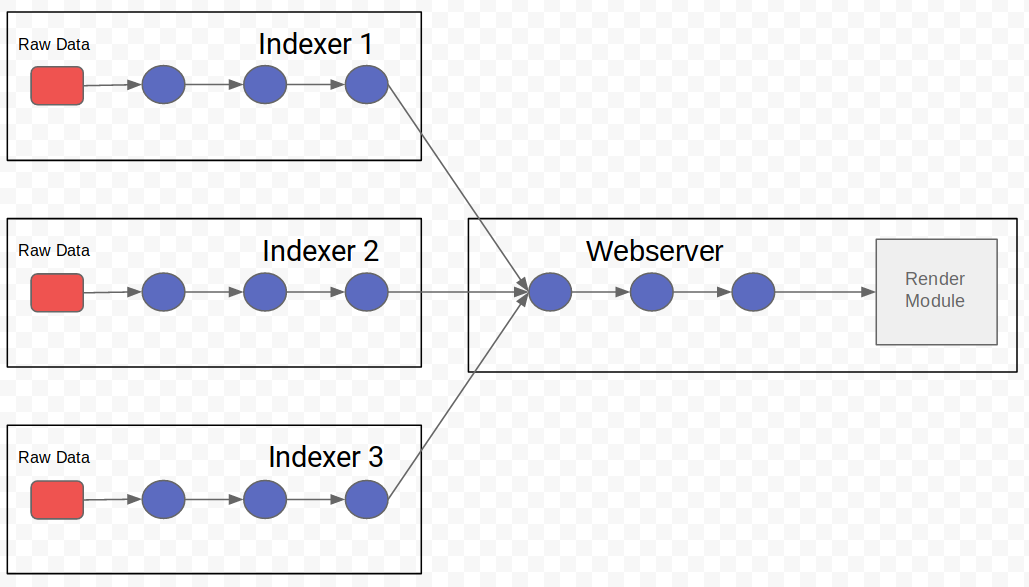
\includegraphics{images/pipeline.png}
	\caption{The Gravwell pipeline}
	\label{fig:pipeline}
\end{figure}


%%%%%%%%%%%%%%%%%%%%%%%%%%%%%%%%%%%%%%%%%%%%%%%%%%%%%%%%%%%%%%%%%%%
% TODO: Exhaustive sections detailing what a tag is, what an entry is,
% what a search module is, what a renderer is
%%%%%%%%%%%%%%%%%%%%%%%%%%%%%%%%%%%%%%%%%%%%%%%%%%%%%%%%%%%%%%%%%%%


\section{Query Entries and Tags}
\index{Search!entries}\index{Entries}\index{Tags}
The first part of any query is the \emph{tag set}; all queries operate on at
least one tag, but a single query can operate on multiple tags. If no
tag is specified, the \code{default} tag is assumed. Every entry in
Gravwell is assigned a tag when it is ingested. The tags control which
well the entry is stored in and are kept with the entry throughout the
entire query pipeline. To specify a set of tags for a specific query,
prepend the query with \code{tag=} and a comma-separated list of tags. For
example, if we wanted to examine all entries that have been assigned the
tags ``syslog'' and ``kernel'' we would prepend our query with
\code{tag=syslog,kernel}. Tags can also be specified using glob wildcards,
so if our Gravwell deployment has data tagged ``syslog'', ``system'', and
``netflow'' we can select the tags ``syslog'' and ``system'' (excluding ``netflow'') by using
\code{tag=sys*}. 

The query \code{tag=*} instructs Gravwell to just go get all the entries,
from every tag, and push them into the \code{text} renderer (the default renderer).
A word of warning: if your system
has lots of data and you run this query over a long period of time, you are
basically asking all your indexers to dump their raw data to the
webserver and hand it to your web browser. This will put a lot of traffic on
the network and consume a lot of resources on the indexers and webserver.

We can expand on this query and use the \code{TAG} and \code{DATA} keywords to draw a
table with the raw data and tag name. You can always access the human
readable name of a tag through the TAG keyword.

\code{tag=* table TAG DATA}

Figure \ref{fig:tag-data-table} shows an example of the output from this search. The table renderer will attempt to present data as a text, but since
the data tagged as \code{pcap} is binary (actual packets) it can't really
be printed as text, thus the ``noise''. Later in this chapter, we will show how to
process this binary data.

\begin{figure}
	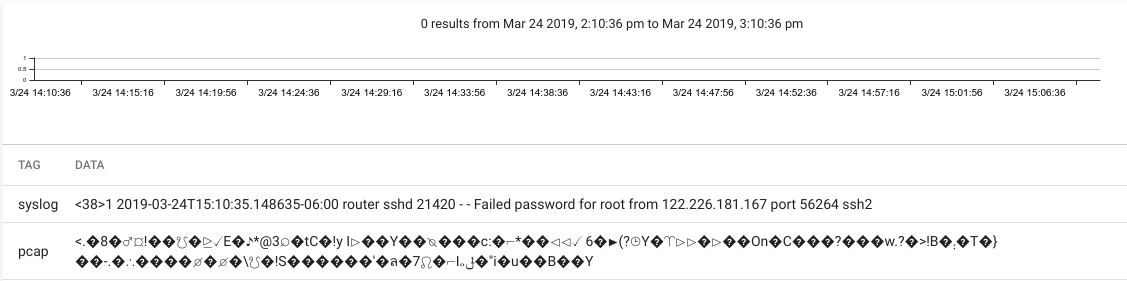
\includegraphics{images/table-tag-data.png}
	\caption{Table showing tags and raw data}
	\label{fig:tag-data-table}
\end{figure}
\clearpage




\section{Chaining Multiple Modules}

Gravwell search modules are each designed to accomplish a specific
task; the power of Gravwell is obtained by chaining multiple modules
together to accomplish something complex. Modules are chained together
using the pipe character ``\textbar{}''. You can chain as many modules
together as you want. The Gravwell pipeline is designed to be
asynchronous, with each module runs in its own lightweight thread. This
means that if you build a query with 8 modules chained together, the
query can potentially leverage 8 CPU cores for the work. This
asynchronous execution allows Gravwell to leverage modern processors
with many CPU cores. It also makes for faster execution even though each
query module does not execute at the exact same speed. If you are
familiar with a Unix command line and chaining multiple programs
together to achieve a result, Gravwell will feel like second
nature--the Gravwell pipeline is directly modeled on the Unix command
line.

Let's examine a query that uses successive filtering modules to find
syslog data from a specific service originating from a specific machine.
We will use the
\code{grep} module
twice, first filtering for the machine name and then filtering for the
service name. Gravwell's \code{grep} module behaves much like the Unix tool of the same name: it searches text for patterns the user specifies. See \href{https://docs.gravwell.io/\#!search/grep/grep.md}{https://docs.gravwell.io/\#!search/grep/grep.md} for more information or refer to Section \ref{sec:grep}. Our example query is:

\code{tag=syslog grep dunkel \textbar{} grep sshd}

This query tells all indexers that we only want to look at syslog
data (\code{tag=syslog}). The first \code{grep} search module filters out all entries which do not
have the value ``dunkel'' (a hostname) in their data. The second \code{grep} filters out all
entries which do not have the value ``sshd'' in their data. The output
entries are guaranteed to contain both ``dunkel'' and ``sshd'' in their
bodies.

Therefore, given the following entries as input, the first one would be returned while the second would be dropped:

\begin{Verbatim}[breaklines=true]
Mar 20 17:41:08 dunkel sshd[26779]: Failed password for root from 218.92.0.192 port 38978 ssh2
Mar 20 17:41:05 porter sshd[21703]: Failed password for root from 218.92.0.192 port 57623 ssh2
\end{Verbatim}

However, the query as you see it is not what actually gets executed.
Our example query does not specify a \emph{renderer} module, so Gravwell
transparently appends the default text renderer. The search pipeline
also detected that there were no condensing modules and the renderer did
not report that it could condense, so it also injected ``sort by time
desc'' so that all the entries are shown in the correct temporal order.
The actual executed query is:

\begin{Verbatim}[breaklines=true]
tag=syslog grep build | grep sshd | sort by time desc | text
\end{Verbatim}

You don't need to really worry about the injected modules and the
default renderer, just know that if you don't specify a renderer
Gravwell will show you the raw entries and ensure they are in the
correct order.

\subsection{The grep Module}
\label{sec:grep}\index{grep}
Grep is a very basic pipeline module that searches for a text string (not Unicode). Any record containing such text will match and be passed through the pipeline. Any record not containing the text is dropped from the pipeline. For example, \code{grep foo} will pass on any records containing the text ``foo'' and drop any records that do not contain ``foo'' anywhere. Grep is case sensitive by default, so \code{grep foo} would match ``foo'' but drop ``Foo''.

Grep supports the standard GNU wildcards as well as fast string and binary matching. For instance to look for all entries that start that contain ``foo'' and ``bar'' separated by 0 or more bytes, you can use \code{grep foo*bar}.

Grep allows multiple patterns to be specified. If any pattern is matched, the entry is passed down the pipeline. If the -v flag is used to invert the search, the entry will be dropped if any pattern matches.

The module supports the following option flags:

\begin{itemize}
\item \code{-v}: ``Inverse'' grep. For instance, \code{grep -v bar} would drop any records containing the text ``bar'' and pass on any records that do not contain ``bar''.
\item \code{-i}: Match case insensitive values. Thus, \code{grep -i foo} would match ``Foo'' and ``foo''. Case insensitive search tends to be one of the slowest operations; put it later in your pipeline if possible to keep things fast.
\item \code{-e <arg>}: Operate on an enumerated value instead of on the entire record. For example, to show packets that contain HTTP text but aren’t destined for port 80, run \code{tag=pcap packet ipv4.DstPort!=80 tcp.Payload | grep -e Payload "GET / HTTP/1.1"}
\item \code{-s}: Strict match. All patterns must match, or in the case of a negated strict match, no pattern may match.`
\item \code{-simple}: Simple match. With this flag, grep will match exactly the characters you specify, with no wildcard matching. This allows you to find asterisks and other normally-reserved characters: \code{grep -s *}
\item \code{-w}: Word match. The entire match pattern must be a full word as would be matched by the fulltext extractors.
\end{itemize}

\clearpage
\subsection{Hands-on Lab: Basic Filtering}
\label{sec:lab-filter}

For this hands-on lab we are going to chain a few modules together to
achieve some basic filtering and zero in on very specific data.

Start by cleaning your environment and starting up a new base Gravwell
instance:

\begin{Verbatim}[breaklines=true]
docker stop $(docker ps -q)
docker rm $(docker ps -q -a)
docker create --rm --net gravnet -p 8080:80 --name test gravwell:base
docker start test
\end{Verbatim}

Next, we'll use the \code{reimport} ingester to ingest a prepared set of logs into the \code{syslog} tag:

\begin{Verbatim}[breaklines=true]
cd ~/gravwell_training/Search/Lab-Basics
docker run -v $PWD/data:/tmp/data --rm -i --net gravnet \
gravwell:ingesters /opt/gravwell/bin/reimport -rebase-timestamp \
-clear-conns test -i /tmp/data/auth.json.gz -import-format json
\end{Verbatim}

Log into your Gravwell GUI (\href{http://localhost:8080}{http://localhost:8080}, recall that the username/password is ``admin''/``changeme'' by default), then try the following tasks:

\begin{enumerate}
\item
  Using the \code{grep} module, filter the syslog tag to only include logs from the sshd daemon on the
  host \code{porter}.
	\begin{enumerate}
	\item
	  Hint: Refer back to the section above for example queries you can adapt.
	\end{enumerate}
\item
  Filter the syslog tag to include sshd logs from all hosts \emph{except} \code{porter}.
	\begin{enumerate}
	\item
	  Hint: The grep module has a -v option that inverts the filter logic, meaning any entries which match the pattern will be \emph{dropped}.
	\end{enumerate}
\item
  Filter the syslog tag to find successful logins on the host \code{porter}.
	\begin{enumerate}
	\item
	  Hint: sshd will log ``Accepted'' when a user logs in.
	\end{enumerate}
\item
  Generate a final count of failed ssh password logins for non-root
  accounts.
	\begin{enumerate}
	\item
	  Hint: Use the \code{count} module without any arguments to count entries.
	\end{enumerate}
\end{enumerate}

Do not \code{rm} the test container, as we are
going to use it again for the next lab.

\section{Entries, Enumerated Values, and Field Extraction}
\index{Search!enumerated values}\index{Enumerated Values}
One of the most common operations any Gravwell user will perform is
field extraction. Gravwell is designed to operate on unstructured data,
meaning that you don't necessarily have to understand the form of your data
until you need to actually query it. Field extraction allows us to
isolate and extract the tidbits that we care about and then operate on
them to gain useful insights.

When a field is extracted from an entry, it becomes an \textbf{Enumerated Value}.
Enumerated values are composed of a name, data, and a type. In
most cases, you don't need to worry about the type since Gravwell will
handle the translations and casting for you, but should you run into any
ambiguity in a query the type is there to help Gravwell do the right
thing. When an enumerated value is extracted it is attached to an
entry for the remainder of the pipeline. Entries can have many enumerated values attached.

The best way to demonstrate field extraction and enumerated values is
to perform a few queries and look at the results. Let's look at some
Apache access log data and perform some queries that use enumerated
values. First let's see what a standard Apache combined access
log\footnote{http://httpd.apache.org/docs/2.2/logs.html\#combined} looks like;
note that the entry is a single line of text but has been broken into
several lines for printing here:

\begin{Verbatim}[breaklines=true]
58.71.219.5 - Bayer3954 368 [2019-03-21T11:10:21-06:00] 
"GET /vortals/target/frontend?data=7b22757365726e616d65223
a226a6f65222c2270617373776f7264223a226368616e67656d65227d"
200 58212 "http://www.humanmethodologies.com/aggregate"
"Mozilla/5.0 Chrome/38.0.89"
\end{Verbatim}

The log entry is pretty complex and contains several pieces of data
that might be useful to analyze, but first we need to get them out of
that log entry. Let's start by issuing a query that uses the regex
module to extract the requesters IP and username:

\begin{Verbatim}[breaklines=true]
tag=apache regex "^(?P<ip>\S+)\s\S+\s(?P<user>\S+)\s" | table
\end{Verbatim}

\begin{figure}
	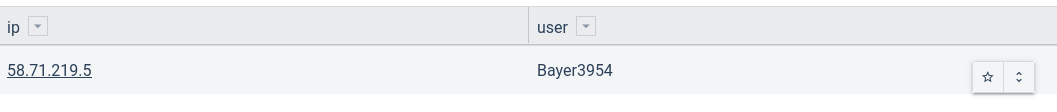
\includegraphics[width=0.8\linewidth]{images/extract-ip.png}
	\caption{Extracted IP and username}
	\label{fig:extract-ip}
\end{figure}

Figure \ref{fig:extract-ip} shows the results.
Note that if you specify the table renderer and don't give it column
names, it will automatically use every enumerated value created in the
pipeline. Our regular expression extracted two features from the log
entry named ``ip'' and ``user'' and attached them to the entry. The
table renderer then created columns using the enumerated value names
and rendered a row for each entry, populating the columns with the
enumerated value names.

We can expand on these extractions by also extracting the method and
URL. Rather than trying to modify our regular expression to extract
everything all at once, let's chain another regular expression that only
extracts those values. This demonstrates that successive modules can
extract additional features and attach them to entries.

\begin{Verbatim}[breaklines=true]
tag=apache regex "^(?P<ip>\S+)\s\S+\s(?P<user>\S+)\s" |
regex "\]\s\"(?P<method>\S+)\s(?P<url>\S+)\"\s"
| table
\end{Verbatim}

\begin{figure}
	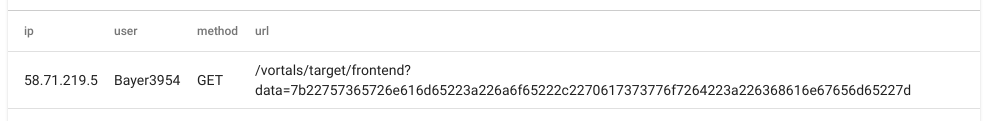
\includegraphics[width=0.8\linewidth]{images/extract-chaining.png}
	\caption{Chaining multiple extractions}
	\label{fig:extract-chaining}
\end{figure}

Now that we have the IP, username, method, and URL, let's extract a
feature from a feature. We will chain yet another module to extract
just the data parameter from the already-extracted URL by adding another
regular expression statement that only operates on the ``url''
enumerated value. This time we'll specify the columns we actually care
about as arguments to the table renderer. Figure \ref{fig:extract-ev} shows
the results of the query.

\begin{Verbatim}[breaklines=true]
tag=apache regex "^(?P<ip>\S+)\s\S+\s(?P<user>\S+)\s" |
regex "\]\s\"(?P<method>\S+)\s(?P<url>\S+)\"\s"|
regex -e url "data=(?P<data>[\da-z]+)" |
table ip user method data
\end{Verbatim}

\begin{figure}
	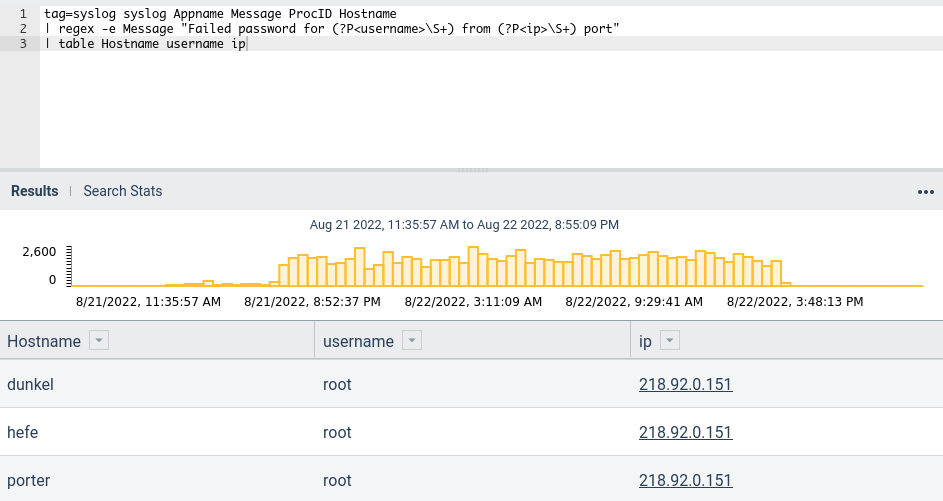
\includegraphics[width=0.8\linewidth]{images/extract-ev.png}
	\caption{Extracting from an enumerated value}
	\label{fig:extract-ev}
\end{figure}

\begin{samepage}
We can see that the data is hex encoded, so let's pass it to the
\code{hexlify}\footnote{https://docs.gravwell.io/\#!search/hexlify/hexlify.md} module
and decode it.

\begin{Verbatim}[breaklines=true]
tag=apache regex "^(?P<ip>\S+)\s\S+\s(?P<user>\S+)\s" |
regex "\]\s\"(?P<method>\S+)\s(?P<url>\S+)\"\s"|
regex -e url "data=(?P<data>[\da-z]+)" |
hexlify -d data as decoded |
table ip user method decoded
\end{Verbatim}
\end{samepage}

\begin{figure}
	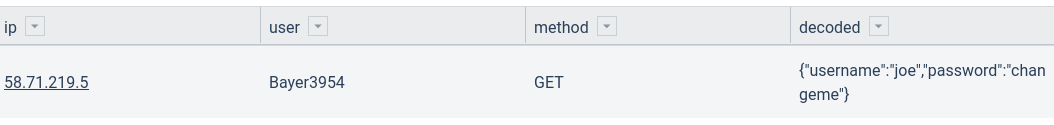
\includegraphics[width=0.8\linewidth]{images/hex-decode-url.png}
	\caption{Hex-decoded URL}
	\label{fig:hex-decode-url} 
\end{figure}


We were able to chain multiple pipeline modules to extract multiple
fields and then operate on those extracted fields to make machine data
consumable by a human. As a result we can see that the user
``Bayer3954'' is performing a GET request and sending URL parameters
that contain encoded JSON data. We can even pass that extracted and
decoded URL data to the \code{json}\footnote{https://docs.gravwell.io/\#!search/json/json.md}
module, extract the username and password fields, and add them to the table as
seen in Figure \ref{fig:url-extract-json}

\begin{Verbatim}[breaklines=true]
tag=apache regex "^(?P<ip>\S+)\s\S+\s(?P<user>\S+)\s" |
regex "\]\s\"(?P<method>\S+)\s(?P<url>\S+)\"\s"|
regex -e url "data=(?P<data>[\da-z]+)" |
hexlify -d data as decoded |
json -e decoded username password |
table ip user method username password
\end{Verbatim}

\begin{figure}
	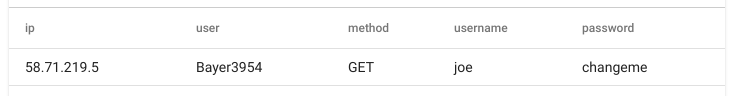
\includegraphics[width=0.8\linewidth]{images/url-extract-json.png}
	\caption{URL parameters extracted as JSON}
	\label{fig:url-extract-json}
\end{figure}

Using our chained modules we were able to take a rather complex Apache
log with encoded data and translate it into an easily-digestible table.
If we were operating in a security context we might set up an alert due
to the fact that the user ``Bayer3954'' is sending requests with someone
else's username (``joe'').

\clearpage
\subsection{Hands-on Lab: Searching with Enumerated Values and Field Extraction}

For this lab we are going to be using the same data set as the previous lab (Section \ref{sec:lab-filter}), but
instead of just filtering we will extract data and output statistics to
zero in on some bad behavior. If you tore down the environment from
previous lab, go back and stand it back up and reingest the auth data.

We will be using some regular expressions to extract data from Linux
auth logs. Because regular expressions can be tricky we will just
provide a few examples to get you started.

This regular expression extracts the hostname and application name which generated the entry into enumerated values named ``host'' and ``app'':

\begin{Verbatim}[breaklines=true]
\S+\s\d+\s\S+\s(?P<host>\S+)\s(?P<app>[^\[]+)\[\d+\]:\s
\end{Verbatim}

This regular expression extracts the message from the syslog entry into an enumerated value named ``msg'':

\begin{Verbatim}[breaklines=true]
\[\d+\]:\s(?P<msg>.+)
\end{Verbatim}

This expression extracts the username (``user'') and IP address (``ip'') from an SSH log entry. It expects to operate on the ``msg'' enumerated value, not the full entry.

\begin{Verbatim}[breaklines=true]
^(?P<action>\S+)\spassword\sfor\s(?P<user>\S+)\sfrom\s(?P<ip>[\d\.]+)\s
\end{Verbatim}

\subsubsection{Lab Tasks}

\begin{enumerate}
\item
  Extract the \code{app} and \code{host} from the entries and put them in a
  table.
	\begin{enumerate}
	\item
	  Add another extraction to pull the \code{msg} portion of the logs and
	  add it to the table.
	\end{enumerate}
\item
  Filter to only include sshd messages by matching on the \code{app} enumerated value.
	\begin{enumerate}
	\item
	  Generate a table with the count of \code{app} events by each \code{host}. Hint: \code{count by host}
	\end{enumerate}
\item
  Extract the \code{ip} and \code{user} for all SSH login events.
\end{enumerate}

\textbf{BONUS}: generate a table with success and failure counts for each IP.

To clean up after the experiment, simply run:

\begin{Verbatim}[breaklines=true]
docker kill $(docker ps -a -q)
\end{Verbatim}


\section{Search Modules}
\index{Search!modules}
Gravwell supports a wide variety of search modules that are designed to
perform various functions. Many of the search modules are used to
perform feature extraction such as \code{json}, \code{syslog}, \code{cef},
\code{csv}, \code{fields}, \code{netflow}, etc. Feature \textbf{extraction modules}
transform raw data into structured data so that features can be
extracted; they are also designed to be specification tolerant. This
means that the modules will often operate on data that doesn't quite fit
the spec. The \code{cef} and \code{syslog} modules are great examples, as there
are specs for syslog (RFC5424) and CEF but almost no one follows them
completely, so the extraction modules have to be tolerant to what is
actually out in the wild.

Gravwell also has many \textbf{analytical modules}. These modules perform
statistical analysis. Examples of these are \code{count}, \code{sum},
\code{mean}, \code{stddev}, \code{variance}, and \code{stats}. The analytical
modules are great for performing analysis to identify
trends, deviences and abnormalities in very large datasets. Many
problems have been identified simply by counting log entries over time.
Other search modules allow for plugging in logic which can allow for
very complicated processing. The \code{eval} module allows for arbitrarily
complex boolean logic, and the \code{anko} module lets you plug a
Turing-complete script into the pipeline. If there isn't a module that
accomplishes exactly what you want to do, Gravwell makes it possible to
drop in your own custom logic via these modules.

Search modules can also perform \textbf{feature enrichment}. Using the
\code{lookup} module we can add external context to data as it goes by
(such as assigning a hostname to an IP). The \code{langfind} module can
use statistical analysis to infer the language of text. Using Gravwell
you might be able to classify users by spoken language using chat logs,
messages, or emails. Gravwell also has modules for complex machine
learning tasks; we used Bayesian inference to generate datasets which
classified social media posts as positive or negative (turns out people
are pretty angry on the Internet). The Gravwell pipeline is designed to
be pluggable and the available search modules are always expanding and
improving. If you can't find what you want and aren't ready to roll
your own using anko, Gravwell may be able to implement the module for you.


\section{Inline Filtering}
\index{Search!filtering}
Many search modules support what we call ``inline filtering''. Inline
filtering allows the module to extract a value and filter on it using
its native type without involving another module. There are some real
benefits to using inline filtering as opposed to extracting in one
module and filtering in another, the most important which may be
acceleration. Search modules that support inline filtering know how to
communicate the filters to an indexer's acceleration engine, which can
enable dramatic speedups. Even when not filtering in a manner that can
invoke the acceleration engine, inline filtering allows for fast type-native operations.

Let's start by examining some modules that support inline filtering and
examine a query that would not invoke the accelerators and then adapt it
so that it can invoke the accelerator. 

Let's begin by examining the data:

\begin{Verbatim}
tag=json
\end{Verbatim}

Here is an example of the data we're looking at:

\begin{Verbatim}[breaklines=true]
{
      "time":"2022-06-08T19:14:31Z",
      "account":{
         "user":"miawilson242",
         "name":"Michael Moore",
         "email":"miawilson242@test.org",
         "phone":"+81 43 3387494435",
         "address":"15 Lincoln Rd,Newstead, OH, 13188", 
         "state":"IA",
         "country":"Brazil"},
      "class":40234,
      "groups":["dagger","jester"],
      "user_agent":"Mozilla/5.0 (Windows NT 6.3; Trident/7.0; rv:11.0) like Gecko",
      "ip":"194.50.167.70",
      "data":"But what sort of language would we have the world speak, if we were told the miracle of Babel was presently to be reversed?"
}
\end{Verbatim}

The data generated is random. To complete this lab, examine the entries and make note of values found for country and groups.
For example, in our sample entry above, we may note the following:
\begin{itemize}
\item country
\subitem "Brazil"
\item groups
\subitem "dagger"
\subitem "jester"
\end{itemize}

In the searches below, make replacements using your pre-selected values.

Let's say we were looking to perform some analytics and we wanted to see
what group activity looked like from users in Brazil. 

Because groups is an array of values, we will extract 
the array and pass the output name to the \code{-x} flag:

\begin{Verbatim}
json -x groups groups account.country
\end{Verbatim}

This will turn the single entry into two entries, one with enumerated values \code{country=Brazil} and
\code{groups=dagger}, one with \code{country=Brazil} and \code{groups=jester}. 

We might write the following query:

\begin{Verbatim}[breaklines=true]
tag=json json -x groups groups account.country | grep -e country Brazil |
count by groups | chart count by groups
\end{Verbatim}

This query will show us a plot of activity groups that are registered
in Brazil. But what if we
have hundreds of thousands of users making making thousands of requests
per day, literally hundreds of millions or billions of JSON records
generated and ingested by Gravwell? Gravwell will handle those numbers,
but the above query will not invoke the accelerators and as a result
hundreds of millions of log entries we don't care about will be read off the disks.
We can make a small adaptation to the query that will:

\begin{enumerate}
\item
  Let the \code{json} module inform the indexer about a filter (invokes
  acceleration).
\item
  Let the \code{json} module filter directly without extracting and
  passing every value.
\end{enumerate}

\begin{Verbatim}[breaklines=true]
tag=json json -x groups groups account.country==Brazil | count by groups |
chart count by groups
\end{Verbatim}

The new query doesn't look much different and the output is identical,
but the performance may be dramatically different. If we have indexed
on the \code{country} field, the json module can tell the acceleration system
about our filter. As a result, only entries that have a country value of
``Brazil'' are ever retrieved from the disk or enter into the
pipeline.

Table \ref{table:filter-ops} shows the filtering operations supported by Gravwell. Note that the greater than/less than operations can only operate on numeric enumerated values; Table \ref{table:filter-compatibility} shows which enumerated value types are compatible with which filters. In this context, ``subset'' means that the enumerated value \emph{contains} the argument, so \code{foo\textasciitilde "well"} would match the strings ``well'', ``wellbeing'', and ``Gravwell''.

\begin{table}[H]
\begin{tabular}{ll}
\textbf{Operator} & \textbf{Name} \\
\hline
\code{==} &	Equal \\
\code{!=} &	Not equal  \\
\code{<} &	Less than  \\
\code{>} &	Greater than \\
\code{<=} &	Less than or equal \\
\code{>=} &	Greater than or equal \\
\code{\textasciitilde} &	Subset \\
\code{!\textasciitilde} &	Not subset \\
\end{tabular}
\caption{Filter operations}
\label{table:filter-ops}
\end{table}

\begin{table}[H]
\begin{tabular}{ll}
\textbf{Enumerated Value Type} & \textbf{Compatible Filters} \\
\hline
string & \code{==}, \code{!=}, \code{\textasciitilde}, \code{!\textasciitilde} \\
byte slice & \code{==}, \code{!=}, \code{\textasciitilde}, \code{!\textasciitilde} \\
MAC address & \code{==}, \code{!=} \\
IP address & \code{==}, \code{!=}, \code{\textasciitilde}, \code{!\textasciitilde} \\
integer & \code{==}, \code{!=}, \code{<}, \code{>}, \code{<=}, \code{>=} \\
floating point & \code{==}, \code{!=}, \code{<}, \code{>}, \code{<=}, \code{>=} \\
boolean & \code{==}, \code{!=} \\
duration & \code{==}, \code{!=}, \code{<}, \code{>}, \code{<=}, \code{>=} \\
\end{tabular}
\caption{Filter compatibility}
\label{table:filter-compatibility}
\end{table}

The subset and not-subset operators have a special meaning when the enumerated value is an IP address: they check if the IP address is part of a \emph{subnet}. Thus \code{ip\textasciitilde 192.168.0.0/16} evaluates to true \emph{if} the value in \code{ip} is in the 192.168.0.0/16 subnet.

If we haven't indexed on the \code{country} field, we still get a speedup
because the filter allows the json module to be more efficient. The
\code{json} module has to walk the data and find each field it is asked to
extract, but by specifying a filter directly in the json module it can
stop execution if one of the extractions fails the filter. In the above
query example, let's say it extracts the country field and gets ``Mexico'';
with inline filtering the json module knows that this fails the
filter, so it stops processing the entry; the \code{group} extraction is
never even performed.

Let's look at another query where inline
filtering lets us perform a filter that is more complex than simple
equality, where the processing module can leverage its knowledge about
the data to do something more interesting. Netflow is a network monitoring data format that generates flows
(records of network connections) from raw network traffic. It can passively watch a network and say that
IP A sent X bytes to IP B using the port Z. So instead of capturing
potentially trillions of bytes for network statistical monitoring, we can
capture just a few. Many smart switches and routers will natively
export netflow.
Using the netflow\footnote{https://docs.gravwell.io/\#!search/netflow/netflow.md} search
module, we can parse the binary Netflow format and do some analysis:

\begin{Verbatim}[breaklines=true]
tag=netflow netflow Src~192.168.0.0/16 DstPort < 1024 |
count by Src DstPort | table Src DstPort count
\end{Verbatim}

For this query we are leveraging the fact that the \code{netflow} module
knows it is dealing with an IP and port; this allows us to apply a
filter with the context of those types. This query is applying a filter
that says we only want flow records where the source IP address is in
the Class B subnet 192.168.0.0 and where the destination port is a
service port (below 1024). These inline filters are not equality
filters, so they will not invoke the accelerators.

Inline filters also have one other trick: some of them can examine two
different fields and extract the one that matches a filter. Assume we
are monitoring Netflow on an internal network and we want to see all
flows that use SSH. We don't care if the flows are inbound or outbound,
but in order to filter for SSH we need to filter on either the SrcPort
or the DstPort. The netflow module lets us specify that a filter match
either the SrcPort \emph{or} the DstPort by just specifying ``Port''. We can do the
same thing for the Src and Dst IP addresses by just specifying ``IP''. So, if we wanted to adapt
the above query to show us any internal private IP that is using
SSH, it would look like this:

\begin{Verbatim}[breaklines=true]
tag=netflow netflow IP~PRIVATE Port==22 Bytes |
sum Bytes by IP | chart sum by IP
\end{Verbatim}

This query also uses the PRIVATE keyword, which tells netflow we are
looking for any non-routable
IP\footnote{https://en.wikipedia.org/wiki/Private\_network\#Private\_IPv4\_addresses} addresses.
Also, even though we are using the Port field that can examine and use
either the SrcPort or DstPort, because we are using an equality filter
it will invoke the accelerator (if we are accelerating on the field).
If we were on a large network with many billions of flows per day, the
accelerators would dramatically speed up that query, plus we get a cool
chart to show us who is pushing a bunch of data around using SSH.

\clearpage
\subsection{Hands-on Lab: Inline Filtering}

In this lab we will observe how the inline
filtering system can improve query performance and simplify the query,
especially when combined with acceleration (see Section \ref{sec:acceleration} for more information
on acceleration).

First, we'll get into the lab subdirectory, then stop and remove any existing containers:

\begin{Verbatim}[breaklines=true]
cd gravwell_training/Search/Lab-Filtering/
docker kill $(docker ps -a -q)
docker rm $(docker ps -a -q)
\end{Verbatim}

Create a new container using the gravwell:base image, upload our lab-specific
configuration file, and restart the container.

\begin{Verbatim}[breaklines=true]
docker create --rm --net gravnet -p 8080:80 --name test gravwell:base
docker cp config/gravwell.conf test:/opt/gravwell/etc/gravwell.conf
docker restart test
\end{Verbatim}

Now we'll use the generators image to generate some JSON data; if you don't have the \code{gravwell:generators} image, see Section \ref{sec:load-lab-images} for instructions on how to load it.

\begin{Verbatim}[breaklines=true]
docker run --net gravnet --rm -it gravwell:generators \
/jsonGenerator -clear-conns test:4023 -entry-count 500000
\end{Verbatim}

Open your Gravwell GUI (\href{http://localhost:8080}{http://localhost:8080}) and check
that there is a new well named ``json'' with 500k entries in it.

Let's start with a query which chains several modules together to
filter in order to get a chart of user activity for all users that are
registered in the country Mexico. We will use the json module to
extract the country and email members, then filter it using the grep
module to only look at users that are registered in Mexico and are using
an email address from \code{example.com}.

Execute the following query:

\begin{Verbatim}[breaklines=true]
tag=json json account.country account.email | grep -e country Mexico |
grep -e email "@example.com" | count | chart count
\end{Verbatim}

This query requires that the json module process every single entry,
extract the country and email fields, and pass it to the grep module
for filtering. We can verify that the pipeline processed 500,000
entries by clicking on the stats tab of the query results.

\subsubsection{Lab Tasks}

\begin{enumerate}
\item
  Adapt this query to use the \code{json} module's inline filtering.
	\begin{enumerate}
	\item Eliminate both greps.
	\item Compare the time required for the query to using grep.
	\end{enumerate}
\item
  Create a new query that generates a list of all users in the group
  ``dagger'' and from the country Canada.
\item
  Adapt the query to generate a count of unique users in the
  group ``dagger'' for each country sorted by largest count first.
\end{enumerate}

If these queries do not yield results, review the data or your list
of pre-selected values. Adapt the query to search for a different group or country.

To clean up after the experiment, simply run:

\begin{Verbatim}[breaklines=true]
docker kill $(docker ps -a -q)
\end{Verbatim}





\clearpage
\section{Render Modules}
\index{Search!renderers}
Gravwell provides a selection of render modules to help users display
their results in the most comprehensible manner possible. Render modules
are in charge of receiving data from the search module pipeline and
organizing it for display to the user. When possible, the renderers
provide a second order temporal index, which allows the user to move
around and zoom in on time spans within the original search. Renderers
can optionally save search results, which can be reopened for later
viewing or even passed to another instance of Gravwell. This is useful
for archiving a view of data or saving the results even after the
original data is expired or purposefully deleted.

\subsection{Temporal vs. Non-Temporal Rendering}
\index{Search!temporal vs. non-temporal}
In discussing renderers, a distinction should be made between temporal
and non-temporal mode. Most searches will operate in \emph{temporal mode},
where the entries arrive at the renderer in order of their
timestamp. This allows the renderer to display a timeline at the top
of the results; the user can select portions of the timeline to zoom in
on a particular subset of the results, as shown in Figure \ref{fig:temporal-render}

\begin{figure}
	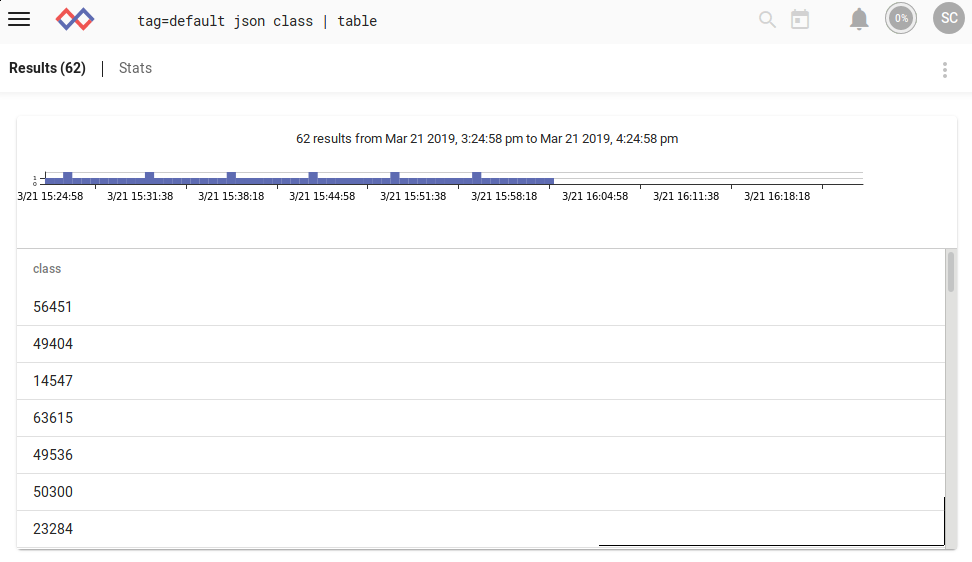
\includegraphics[width=0.8\linewidth]{images/temporal-render.png}
	\caption{Renderer in temporal mode}
	\label{fig:temporal-render}
\end{figure}

If, however, the entries are sorted by something other than time, the
renderer will enter \emph{non-temporal} mode, in which subselection is not
possible, as shown in Figure \ref{fig:nontemporal-render}.

\begin{figure}
	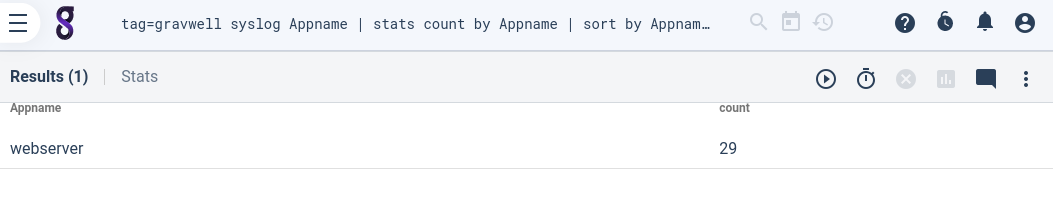
\includegraphics[width=0.8\linewidth]{images/nontemporal-render.png}
	\caption{Renderer in non-temporal mode}
	\label{fig:nontemporal-render}
\end{figure}

\clearpage
\subsection{Hands-on Lab: Temporal vs. Non-Temporal Rendering}

In this hands-on lab we will use netflow records to identify the top
communicating hosts both outbound and inbound from our network. First, launch
a Gravwell container:

\begin{Verbatim}[breaklines=true]
docker run --rm --net gravnet -p 8080:80 -d --name gravwell gravwell:base
\end{Verbatim}

Next, start the ingester container running the netflow ingester:

\begin{Verbatim}[breaklines=true]
docker run --rm --net gravnet --name ingesters -it \
-e GRAVWELL_CLEARTEXT_TARGETS=gravwell:4023 \
gravwell:ingesters /opt/gravwell/bin/gravwell_netflow_capture
\end{Verbatim}

The netflow ingester is pre-configured to listen on port 2055 for
incoming Netflow v5 records.

Now, we use another Docker container to generate Netflow records and
send them to the ingester:

\begin{Verbatim}[breaklines=true]
docker run -it --net gravnet --rm \
networkstatic/nflow-generator -t ingesters -p 2055
\end{Verbatim}

The netflow generator will run indefinitely, generating flow records,
until killed.

Log into the web GUI (\href{http://localhost:8080}{http://localhost:8080}).
We can now search the netflow data. Issue the following netflow search to convert the binary netflow data
into a readable table of information. There are more fields available to
netflow, but for this example we are only going to referring to some of
them.

\begin{Verbatim}[breaklines=true]
tag=netflow netflow Src Dst Bytes | table
\end{Verbatim}

Netflow provides records of communication flows to and from a host. The
temporal overview chart shows bars indicating the presence of netflow
records over time. Clicking and drag in this chart to zoom in on a spike or
valley will cause Gravwell to display results within that time
range (without re-issuing the search).

For this lab we're trying to answer the question of which hosts are
egressing the most data and which are ingressing the most.

To answer the egress question, we can apply a filter to our netflow
module that specifies non-routable private IP addresses. We want to sum
the number of bytes sent by each private host to a public host.

\begin{Verbatim}[breaklines=true]
tag=netflow netflow Src~PRIVATE Dst!~PRIVATE Bytes
| stats sum(Bytes) by Src | sort by sum desc | table Src sum
\end{Verbatim}

Observe that adding in the \code{sort by sum desc} component removes the
overview chart from the top of the search results screen. This is
because the search is now in non-temporal mode--we are sorting results by
the sum, rather than by time.

To see which hosts are accumulating the most ingress traffic, we change
the query slightly to invert the filtering of private address space in
the netflow module, tell the stats module to sum by \code{Dst} instead of \code{Src},
and finally in table we specify \code{Dst} and the \code{sum}. Notice that the sort
module does not change because it is operating on the enumerated value
\code{sum}, which is created by stats regardless of the field being operated
on.

\begin{Verbatim}[breaklines=true]
tag=netflow netflow Src!~PRIVATE Dst~PRIVATE Bytes
| stats sum(Bytes) by Dst | sort by sum desc | table Dst sum
\end{Verbatim}

\textbf{Note}: The `sort' module causes a search to ``collapse'' and may have
performance impacts if used early on in a search pipeline. It should
generally be the last module before the render module, which is `table'
during this lab. See the query optimization section (\ref{sec:query-optimization}) for more on this topic.

To clean up after the experiment, simply run:

\begin{Verbatim}[breaklines=true]
docker kill $(docker ps -a -q)
\end{Verbatim}


\subsection{Downloading Results}
\index{Search!downloading}\index{Search!renderers}
All renderers allow the user to download results in at least one
format.

\begin{itemize}
\item
  Table: JSON, CSV, Lookup table (Gravwell native format).
\item
  Raw/Text: JSON, CSV, text.
\item
  Chart: JSON, CSV.
\item
  Pointmap/Heatmap: JSON.
\item
  FDG: JSON, CSV.
\item
  Stackgraph: JSON.
\end{itemize}

The table renderer's CSV and lookup table options deserve some extra notes.
Downloading a ``lookup table'' or CSV file
from the table renderer results in a file which can be uploaded to
Gravwell again as a resource and used with the lookup module; this is a
convenient way to export a lookup table to another Gravwell system.


\subsection{Text/Raw Renderers}
\index{Renderers!text}\index{Renderers!raw}
These renderers provide only the most basic functionality but are
useful when doing initial explorations on data. The text renderer is
designed to show human readable entries in a text format, as seen in Figure \ref{fig:text-entries}. Any
non-printable characters will be converted to the `.' character. Text
also fully supports Unicode and can render non-ASCII characters. Text is
the default renderer and is applied if no renderer is specified.

The raw renderer is functionally similar to the text renderer, but does
not attempt to modify or change any non-printable characters. This
renderer hands back the raw record, for better or worse. This renderer
can be useful when passing data back to other tools which need the raw
values, or when you just want to see if your browser can take a stab at
turning packets into emojis.

These renderers have a default limit of approximately 1000 characters per
entry, to prevent accidentally displaying multiple megabytes of raw
data. To increase the maximum length of output add the limit argument, 
e.g. \code{text limit 2048} to display up to 2048 characters.

\begin{figure}
	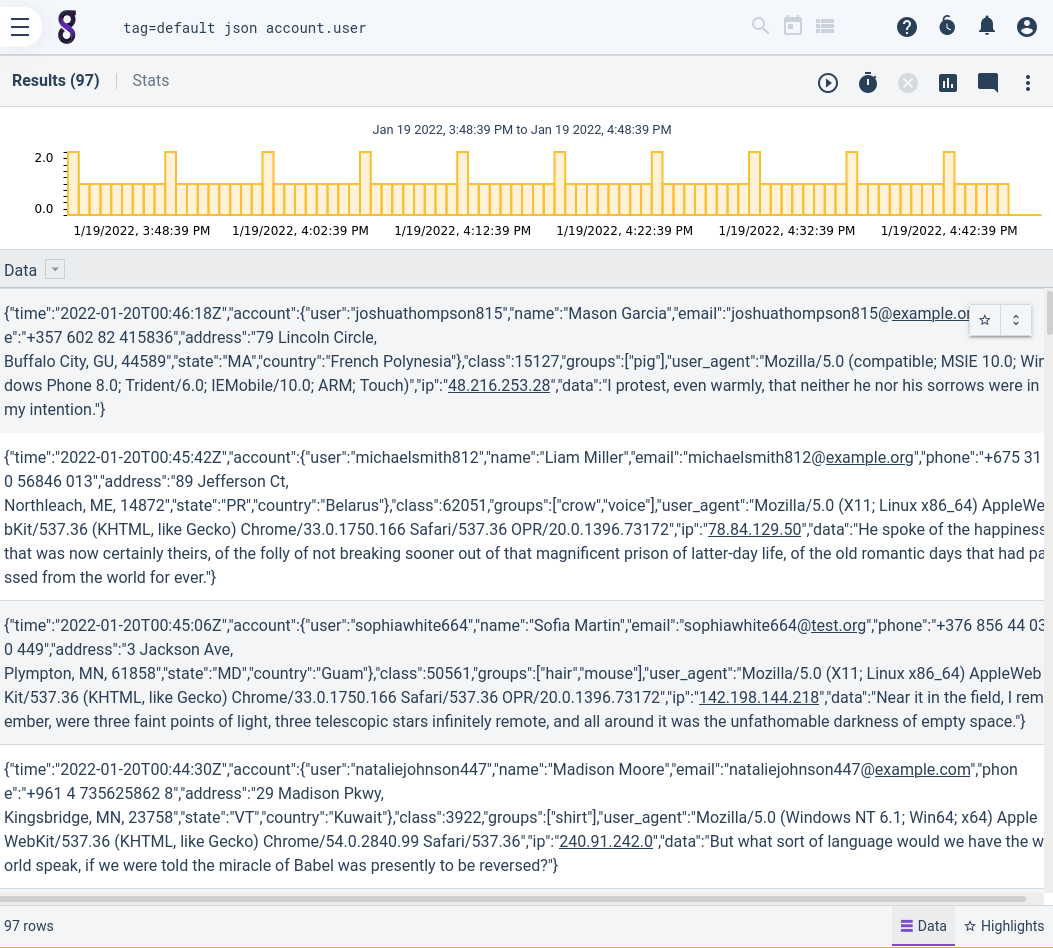
\includegraphics[width=0.7\linewidth]{images/text-entries.png}
	\caption{Text renderer entries view}
	\label{fig:text-entries}
\end{figure}

Hovering the mouse over an entry in the GUI when using either the text
or raw renderer brings up a context menu with two options, as shown
in Figure \ref{fig:text-context-menu}.

\begin{figure}
	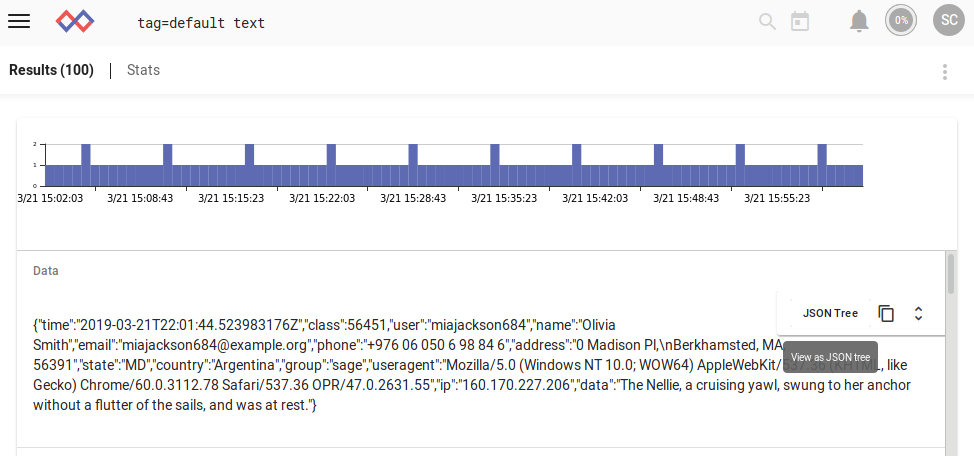
\includegraphics[width=0.7\linewidth]{images/text-context-menu.png}
	\caption{Text renderer context menu}
	\label{fig:text-context-menu}
\end{figure}

The right-most icon shows the built-in fields and any enumerated values on the entry, as seen in Figure \ref{fig:text-ev}. The star icon allows you to highlight particular entries; highlighted entries can be viewed later in the ``Highlights'' tab at the bottom of the page, as seen in Figure \ref{fig:text-highlights}.

\begin{figure}
	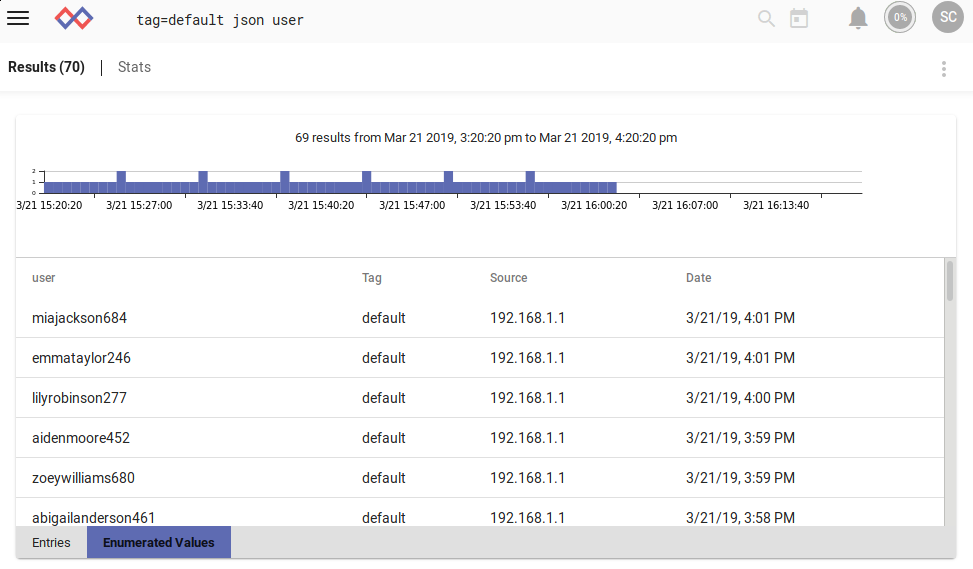
\includegraphics[width=0.7\linewidth]{images/text-ev.png}
	\caption{Text renderer enumerated values view}
	\label{fig:text-ev}
\end{figure}

\begin{figure}
	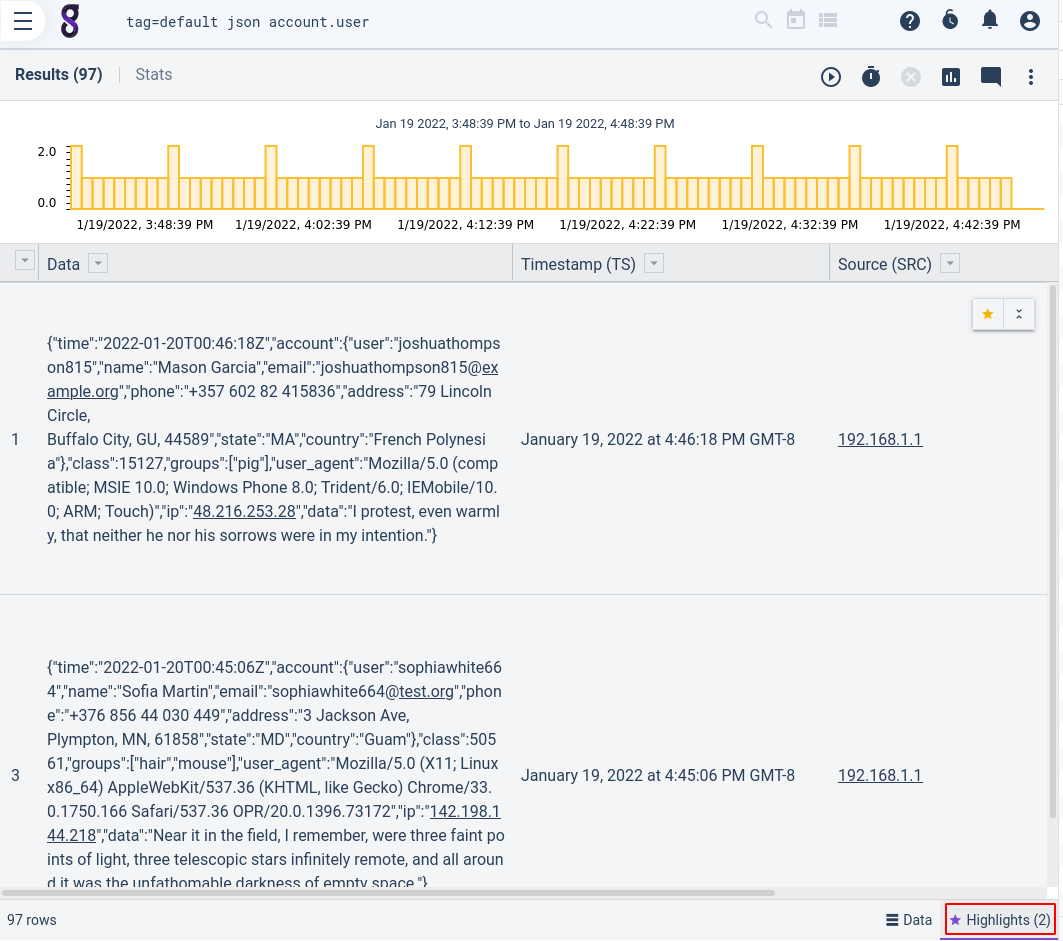
\includegraphics[width=0.7\linewidth]{images/text-highlights.png}
	\caption{Text renderer highlight view}
	\label{fig:text-highlights}
\end{figure}

\clearpage

\subsection{Table Renderer}
\index{Renderers!table}
The table renderer is used to create tables. The renderer's arguments
specify which columns should be shown in the table. Arguments must be
enumerated values, ``DATA'', ``TAG'', ``TIMESTAMP'', or ``SRC''.

Specifying no column arguments causes table to display all enumerated
values as columns instead; this is useful for exploration.

\subsubsection{Supported Options}

\begin{itemize}
\item
  \code{-save \textless{}destination\textgreater{}}: save the resulting table
  as a resource for the lookup module. This is a useful way to save the
  results of one search (say, extracting a MAC→IP mapping
  from DHCP logs) and use it in later searches.
\item
  \code{-nt}: Put the table into non-temporal mode. This causes upstream math
  modules to condense results rather than having table do it. This can
  seriously speed up searches over large quantities of data when
  temporal sub-selection is not needed.
\end{itemize}

\subsubsection{Basic table use}

Extract a few elements from a Netflow record, then have table
automatically display them:

\begin{Verbatim}[breaklines=true]
tag=netflow netflow Src Dst SrcPort DstPort | table
\end{Verbatim}

Find failed SSH login attempts and count how many attempts were made for each username (Figure \ref{fig:table-ssh-bruteforce}):

\begin{Verbatim}[breaklines=true]
tag=syslog grep sshd 
| regex "invalid user (?P<username>\S+)" 
| stats count by username 
| table username count
\end{Verbatim}

\begin{figure}
	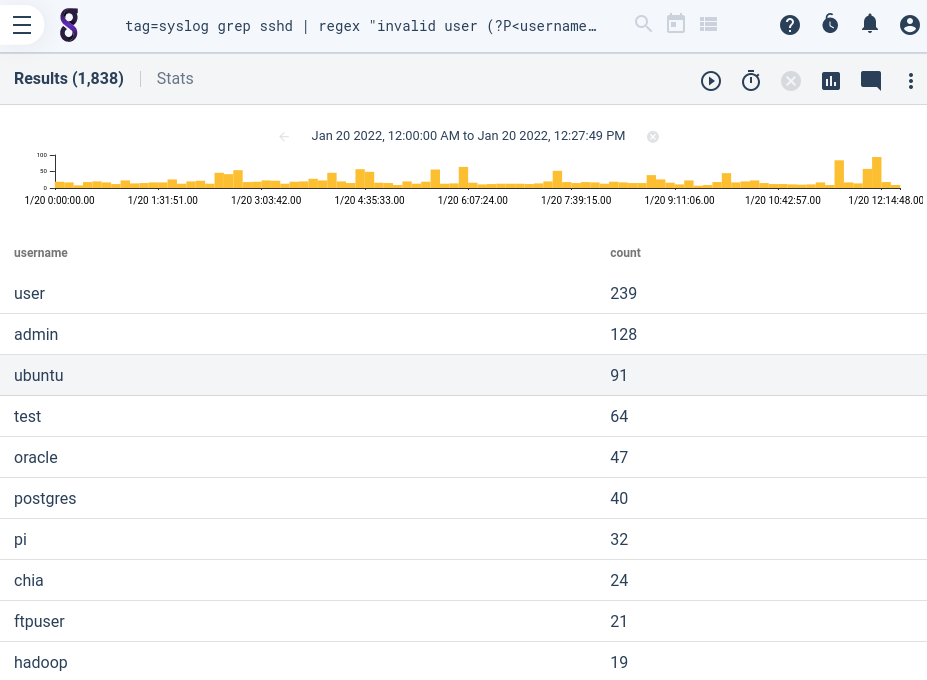
\includegraphics[width=0.7\linewidth]{images/table-ssh-bruteforce.png}
	\caption{Failed SSH login table}
	\label{fig:table-ssh-bruteforce}
\end{figure}

\subsubsection{Using the -save option}

Use DHCP logs to build a lookup table containing IP to MAC mappings:

\begin{Verbatim}[breaklines=true]
tag=syslog regex "DHCPACK on (?P<ip>\S+) to (?P<mac>\S+)"
| unique ip mac | table -save ip2mac ip mac
\end{Verbatim}

Then use the lookup table to find the MACs associated with SSH
logins (results in Figure \ref{fig:ssh-login-macs}):

\begin{Verbatim}[breaklines=true]
tag=syslog grep sshd
| regex "Accepted .* for (?P<user>\S+) from (?P<ip>\S+)"
| lookup -r ip2mac ip ip mac as mac |table user ip mac
\end{Verbatim}

\begin{figure}
	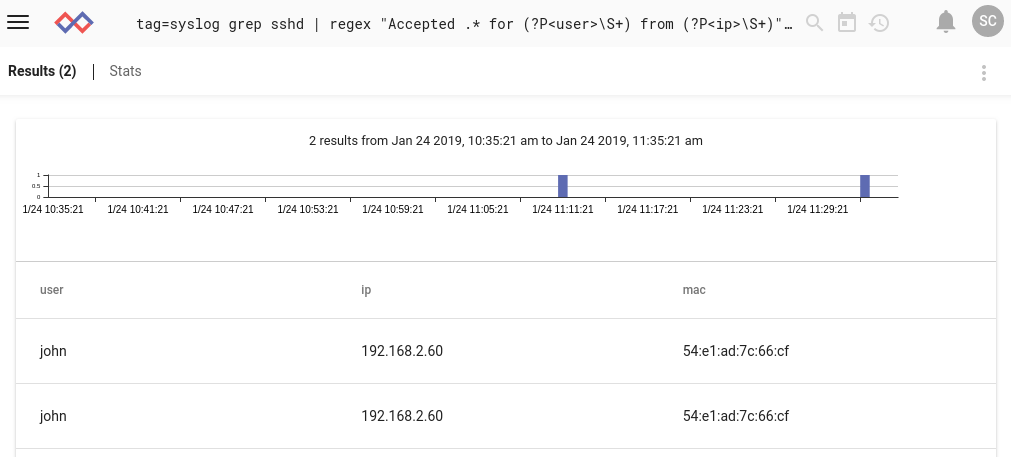
\includegraphics[width=0.7\linewidth]{images/table-ssh-login.png}
	\caption{SSH login MAC addresses}
	\label{fig:ssh-login-macs}
\end{figure}

Refer to the Automation chapter for a detailed description of how the
\code{-save} flag can be used to automatically maintain lookup tables such as
this.

\subsubsection{Using the -nt option}

In a situation with massive quantities of data, this flag will force table into
non-temporal mode, making the \code{count} module condense results instead of table:

\begin{Verbatim}[breaklines=true]
tag=jsonlogs json source | count by source | table -nt source count
\end{Verbatim}

\clearpage

\subsection{Chart Renderer}
\index{Renderers!chart}
The chart renderer is used display aggregate results such as trends,
quantities, counts, and other numerical data. Charting will plot an
enumerated value with an optional ``by'' parameter. For example, if
there are counts associated with names, \code{chart count by name} will
chart a line for each name showing the counts over time. The charting
renderer will automatically limit the plotted lines or bar groups to 8
values. If you would like to see many more lines you can add the \code{limit \textless{}n\textgreater{}}
argument, which tells the charting library
to not introduce the ``other'' grouping until it exceeds the given limit
of n values. The user interface for charting allows for a rapid
transition between line, area, bar, pie, and donut charts.

The following query generates a chart showing the most common invalid usernames seen on incoming SSH connections--indicators of brute-forcing:

\begin{Verbatim}[breaklines=true]
tag=syslog grep sshd 
| regex "invalid user (?P<username>\S+)" 
| stats count by username 
| chart count by username limit 10
\end{Verbatim}

The results can be rendered in a variety of ways. By default, the UI will show a line chart (Figure \ref{fig:chart-line}, but the gear icon on the right side allows you to select a variety of chart types, including pie charts (Figure \ref{fig:chart-pie}.

\begin{figure}
	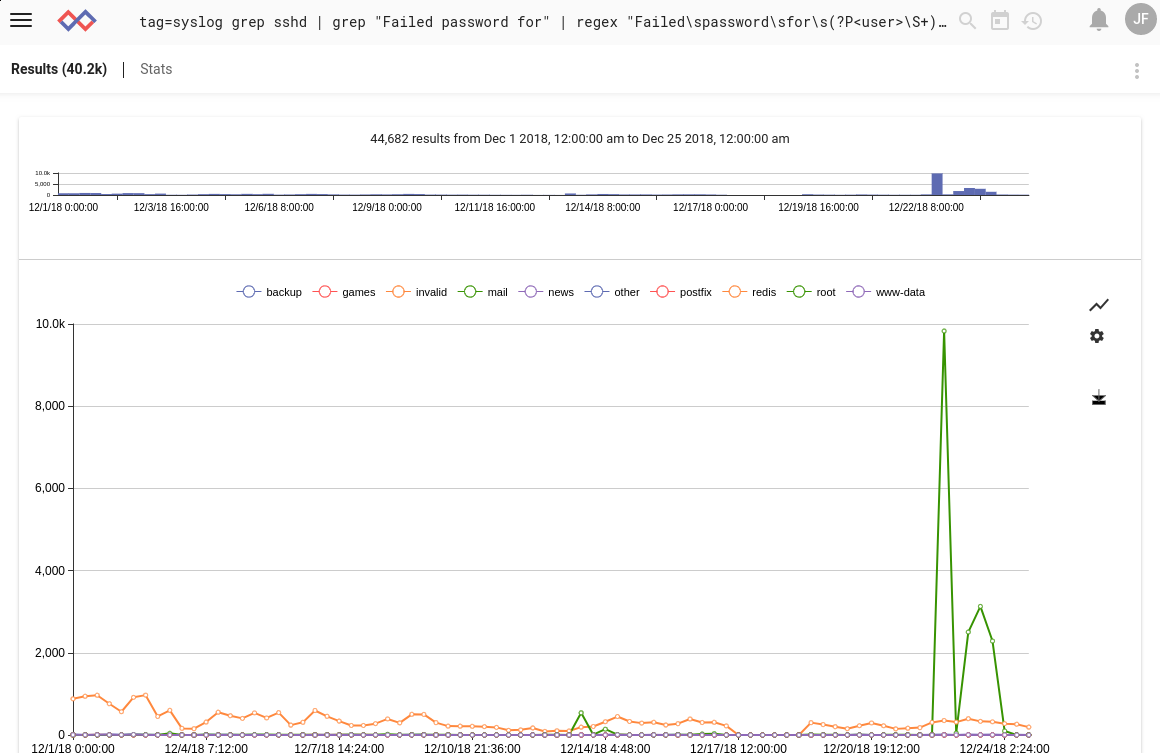
\includegraphics[width=0.6\linewidth]{images/chart-line.png}
	\caption{Line chart}
	\label{fig:chart-line}
\end{figure}

\begin{figure}
	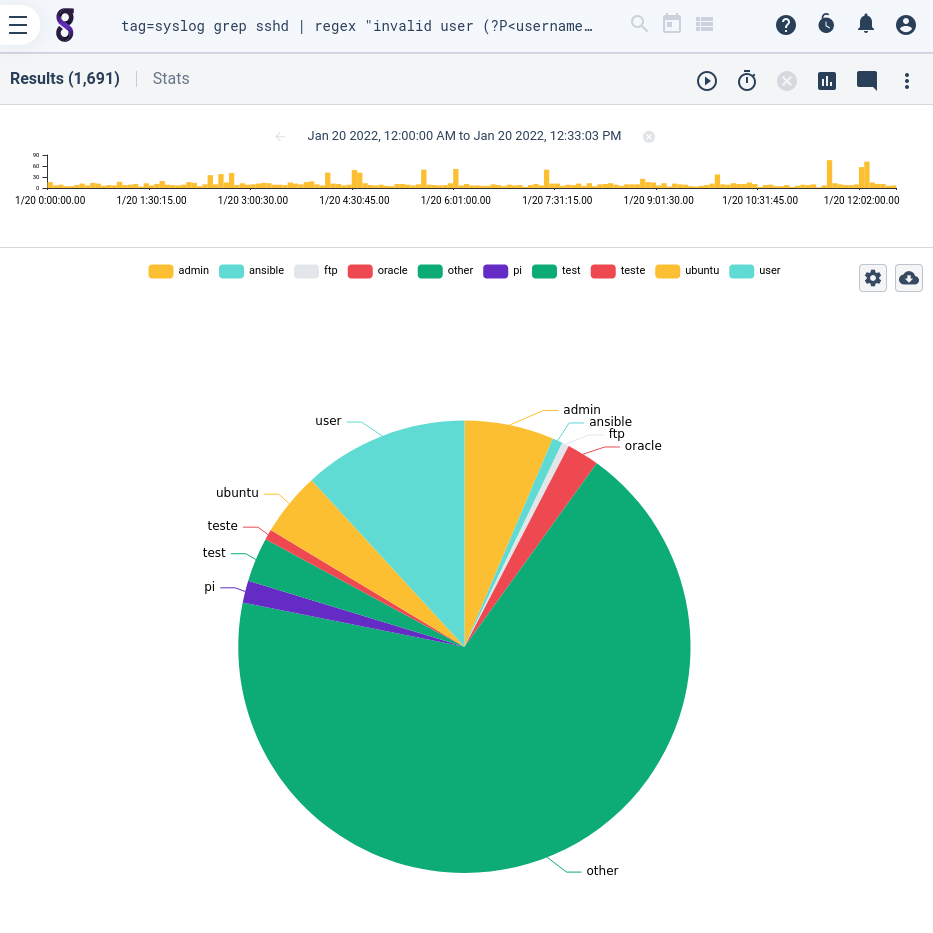
\includegraphics[width=0.6\linewidth]{images/chart-pie.png}
	\caption{Pie chart}
	\label{fig:chart-pie}
\end{figure}

\clearpage

\subsection{Mapping Modules}
\index{Renderers!heatmap}\index{Renderers!pointmap}
The \code{pointmap} and \code{heatmap} renderer modules translate search results onto
a map. Both place entries on the map based on locations in enumerated
values. By default, the modules look for an enumerated value called
'Location', as set by the \code{geoip} search module. Locations can also be
specified explicitly using the following:

\begin{itemize}
\item
  \code{-loc \textless{}enumerated value\textgreater{}} tells the module to
  look for a location in the specified enumerated value, rather than the
  default Location.
\item
  \code{-lat \textless{}enumerated value\textgreater{} -long
  \textless{}enumerated value\textgreater{}} tells the module to look
  for the latitude and longitude values separately. These can be
  floating point numbers (as delivered by the geoip module) or strings
  from another source.
\end{itemize}

The map will display a maximum of 1000 points. It is \emph{geofenced}, meaning
that zooming in on one portion of the map will display up to 1000 points
within that area.

\subsubsection{Pointmap}

Pointmap translates entries into distinct markers on the map. If
additional enumerated value names are specified, their contents will be
displayed when a point is clicked.

The following search displays a map of all IP addresses which connected to the SSH service, as seen in Figure \ref{fig:pointmap-ip}.

\begin{Verbatim}[breaklines=true]
tag=syslog grep sshd | regex "Connection from (?P<ip>\S+) port"
| geoip ip.Location | pointmap ip
\end{Verbatim}

\begin{figure}
	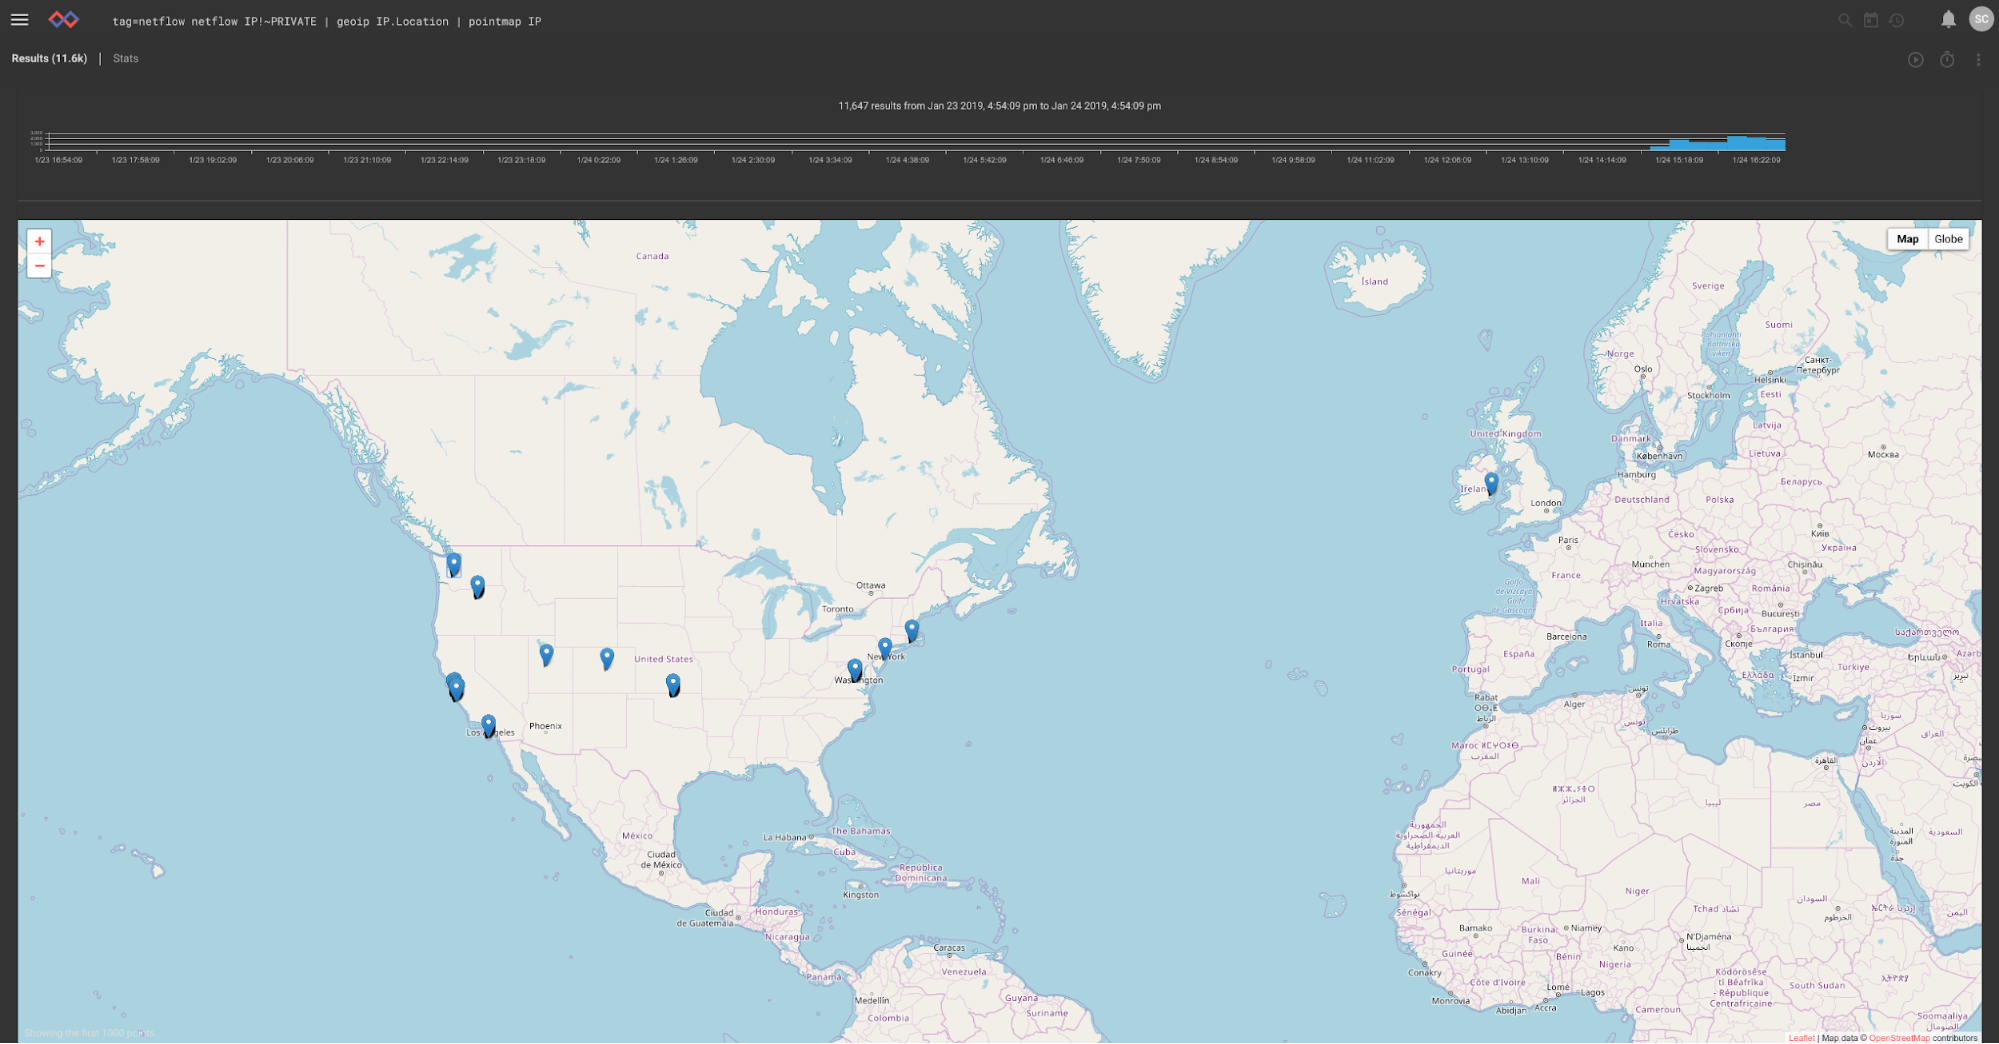
\includegraphics[width=0.6\linewidth]{images/pointmap-ip.png}
	\caption{Pointmap IP locations}
	\label{fig:pointmap-ip}
\end{figure}

We can also use the geoip module to look up an IP address's ASN organization. Any enumerated values passed to the pointmap renderer can be viewed by clicking on a point, as seen in Figure \ref{fig:pointmap2}

\begin{Verbatim}[breaklines=true]
tag=syslog grep sshd 
| regex "Connection from (?P<ip>\S+) port" 
| geoip ip.Location 
| geoip -r asn_db ip.ASNOrg 
| pointmap ip ASNOrg
\end{Verbatim}

\begin{figure}
	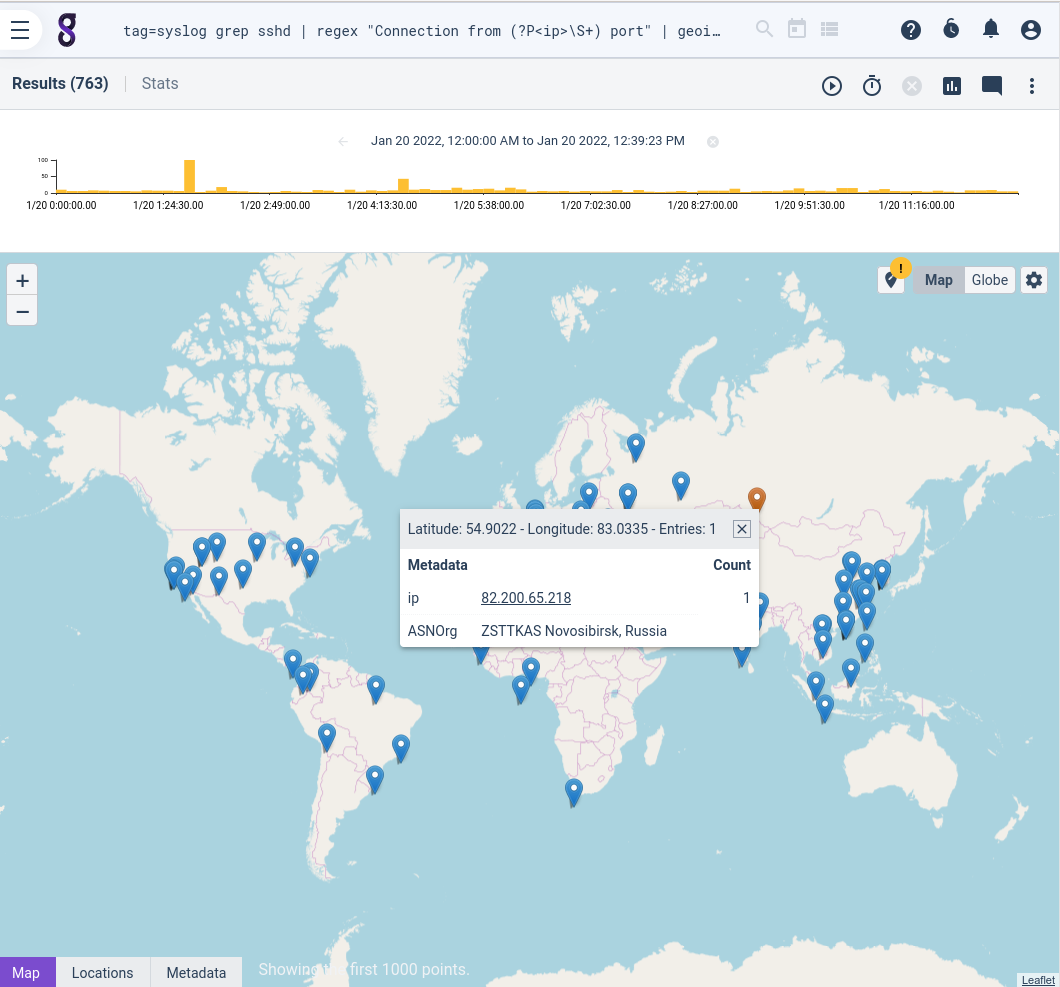
\includegraphics[width=0.6\linewidth]{images/pointmap2.png}
	\caption{Pointmap with additional enumerated values}
	\label{fig:pointmap2}
\end{figure}


\subsubsection{Heatmap}

Heatmap operates similarly to pointmap, but it takes 0 or 1 additional
enumerated values as arguments. If no enumerated value argument is
given, it generates a heat map using the number of entries for each
location as the 'heat'. In this example using IPFIX records, the
'heat' represents the number of connections from a location, as seen
in Figure \ref{fig:heatmap-basic}.

\begin{Verbatim}[breaklines=true]
tag=ipfix ipfix ip!~PRIVATE 
| geoip ip.Lat ip.Long 
| heatmap -lat Lat -long Long
\end{Verbatim}

\begin{figure}
	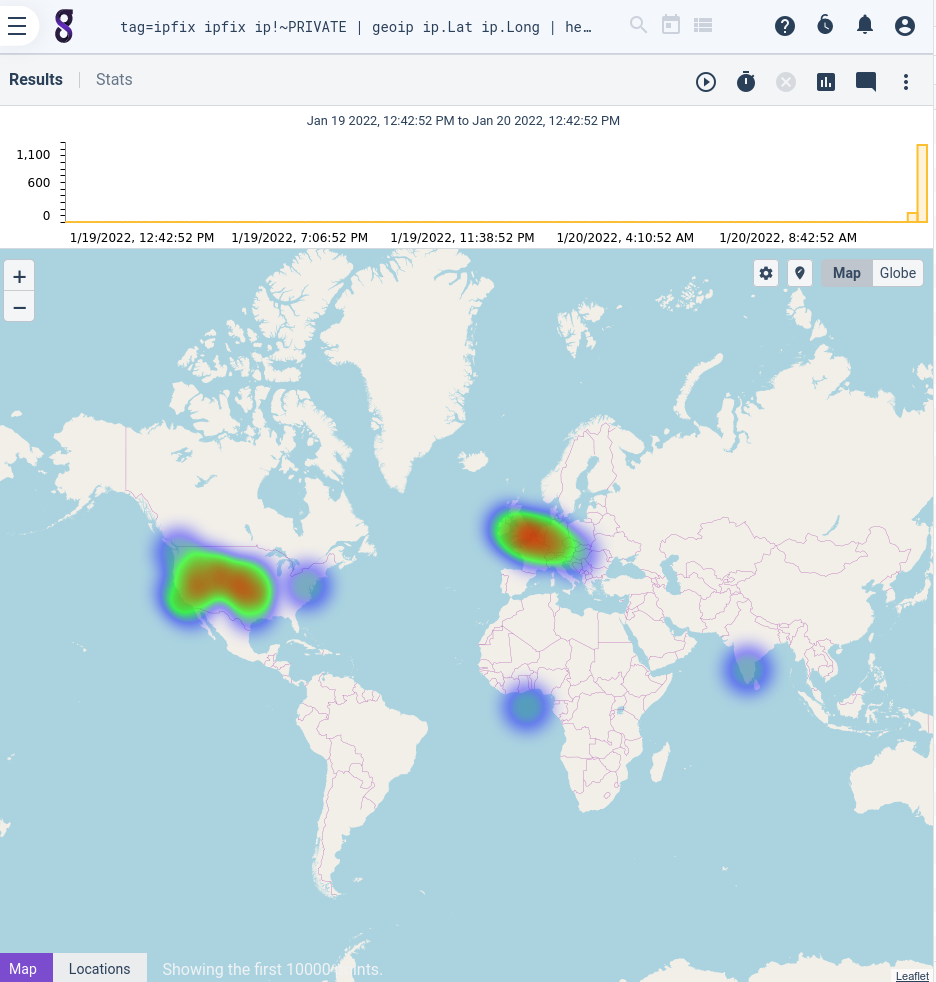
\includegraphics[width=0.6\linewidth]{images/heatmap-basic.png}
	\caption{Basic heatmap use}
	\label{fig:heatmap-basic}
\end{figure}

If we add the total number of bytes as an argument, the 'heat' is
derived from the number of bytes sent over the connection, rather than
the number of connections, as shown in Figure \ref{fig:heatmap-bytes}.

\begin{Verbatim}[breaklines=true]
tag=ipfix ipfix ip!~PRIVATE bytes 
| stats sum(bytes) by ip 
| geoip ip.Location 
| heatmap sum
\end{Verbatim}

\begin{figure}
	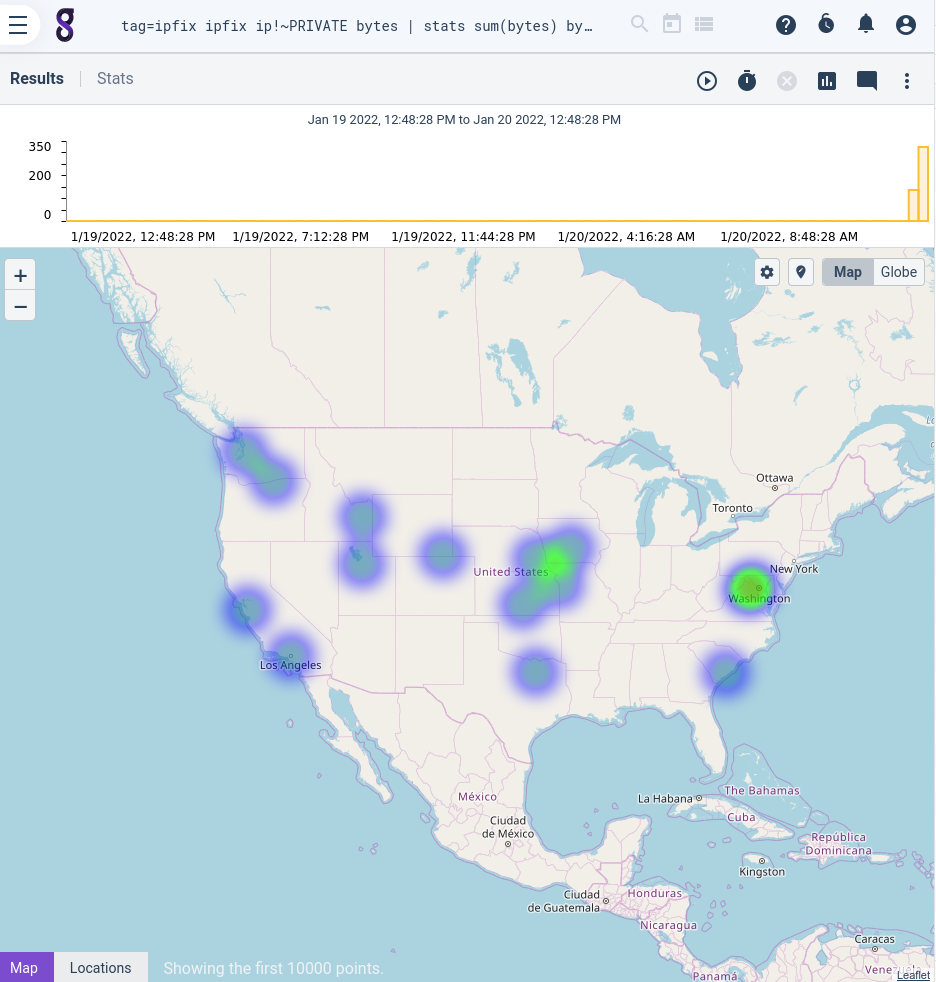
\includegraphics[width=0.6\linewidth]{images/heatmap-bytes.png}
	\caption{Heatmap using byte count as ``heat''}
	\label{fig:heatmap-bytes}
\end{figure}

\clearpage

\subsection{Stackgraph Renderer}
\index{Renderers!stack graph}
The \code{stackgraph} renderer is used to display horizontal bar graphs
with stacked data points. A stackgraph is useful in displaying the
magnitude of results that are accumulated from multiple components
across a set of tags. The stackgraph renderer is an accumulator,
meaning that it can interpret the operation of some upstream search
modules and recalculate the results based on sub selections. In Gravwell
terms, stackgraph supports second order searching and selection.

Stackgraph invocation requires three arguments which must be the names
of enumerated values extracted by upstream search components. Argument
one specifies the enumerated value which names each individual
horizontal bar, for example an IP address. Argument two specifies the
enumerated value which gives the individual components of each
horizontal bar, for example a TCP port. Argument three is the magnitude
value which represents the magnitude component of each stack value
within a horizontal bar. Example magnitude components are count, sum,
stddev, sum, max, and min. The easiest way to understand these arguments
is by examining the examples below.

Note: Sorting data before sending it to stackgraph is unlikely to
achieve the desired outcome. If you had a count of IP→port pairs
and were interested in sorting based on that count and then sending to a
stackgraph (e.g. \code{count by SrcIP,DstPort \textbar{} sort by count
desc \textbar{} table SrcIP DstPort count}), then the first item in the
list might be a port that has a very high count but only for one IP. For
example, say port IP 10.0.0.1 spoke on port 443 with count 10000 but the
next 8 entries are 8 different IPs all using port 80 with counts in the
9000 range, they will dwarf port 443 on the graph.

\subsubsection{Stackgraph Example: Traffic Volumes by IP \& Port}

The following query will generate a stackgraph in which each bar respresents
a single IP address, with components inside each bar representing the number
of bytes sent to different TCP or UDP ports. See Figure \ref{fig:stackgraph-traffic}
for a sample of the output.

\begin{Verbatim}[breaklines=true]
tag=ipfix ipfix src ~ PRIVATE port < 1024 bytes 
| stats sum(bytes) by src port 
| stackgraph src port sum
\end{Verbatim}

\begin{figure}
	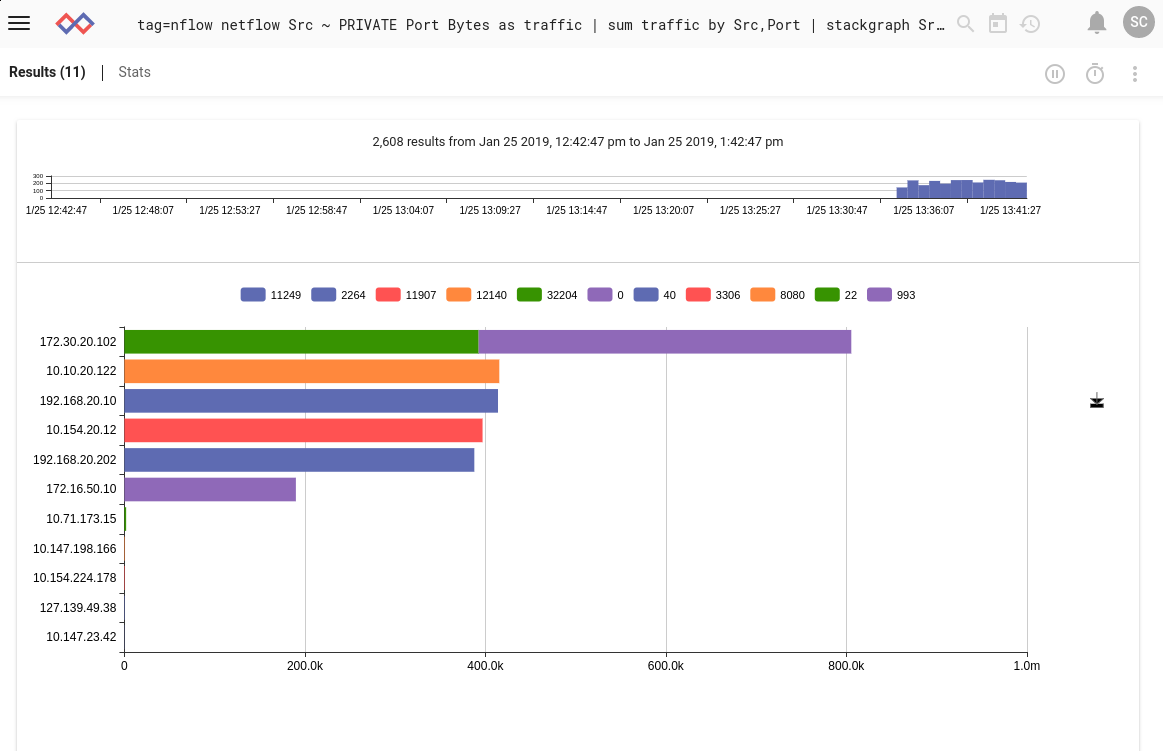
\includegraphics[width=0.6\linewidth]{images/stackgraph-traffic.png}
	\caption{Stackgraph of traffic volumes by IP \& Port}
	\label{fig:stackgraph-traffic}
\end{figure}

\subsubsection{Stackgraph Example: Failed SSH Logins by Country \& User}

This query will generate a stackgraph in which each bar represents a country and the
components of the bars indicate the number of connections to a given port, based on IPFIX logs.
Figure \ref{fig:stackgraph-connections}
shows the results.

\begin{Verbatim}[breaklines=true]
tag=ipfix ipfix ip!~PRIVATE port < 1024 
| geoip ip.Country 
| stats count by port Country 
| require Country 
| stackgraph Country port count
\end{Verbatim}

\begin{figure}
	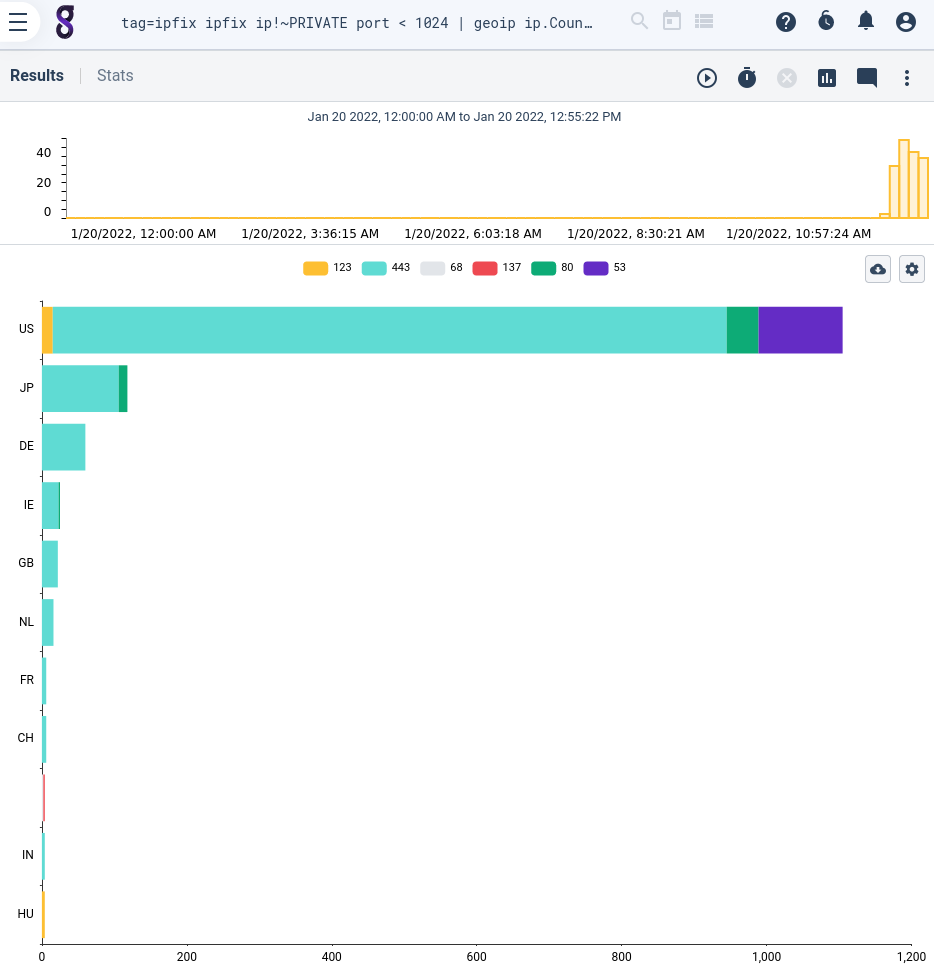
\includegraphics[width=0.6\linewidth]{images/stackgraph-connections.png}
	\caption{Stackgraph of connection count by country \& port}
	\label{fig:stackgraph-connections}
\end{figure}


\clearpage

\subsection{Force-Directed Graph Renderer}
\index{Renderers!force-directed graph}
The force-directed graph (fdg) module is used to generate a directed
graph using node pairs and optional grouping. The fdg module accepts
source and destination groups as well as a weight value for the
resulting edge.

\subsubsection{Supported Options}

\begin{itemize}
\item
  \code{-b}: Indicates that edges are bidirectional, meaning that the pair
  [A, B] is equivalent to [B, A].
\item
  \code{-v \textless{}enumerated value\textgreater{}}: Indicates that edges
  should be weighted as a sum of the provided enumerated value. The -v
  flag is useful in generating directed graphs where edges have weights
  represented by something other than a raw count.
\item
  \code{-sg \textless{}enumerated value\textgreater{}}: Provides a group to
  apply to a source value which is used for coloring a graph. For
  example a source group may be a subnet for an IP which enables nodes
  in a graph to be grouped.
\item
  \code{-dg \textless{}enumerated value\textgreater{}}: Same as -sg, but
  grouping based on destination parameter.
\end{itemize}

\subsubsection{Examples}

Use of the fdg module is easier to demonstrate than to explain. One
example where a force directed graph can prove useful is to identify
relationships between addresses on a network. Generating a weighted
force directed graph of IPV4 traffic while grouping nodes into a class C
network can be accomplished with the following query, as shown in Figure \ref{fig:fdg-classC}.

\begin{Verbatim}[breaklines=true]
tag=pcap packet ipv4.SrcIP ipv4.DstIP ipv4.Length 
| sum Length by SrcIP,DstIP 
| subnet -t SrcSub SrcIP /24 
| subnet -t DstSub DstIP /24 
| fdg -v sum -sg SrcSub -dg DstSub SrcIP DstIP
\end{Verbatim}

\begin{figure}
	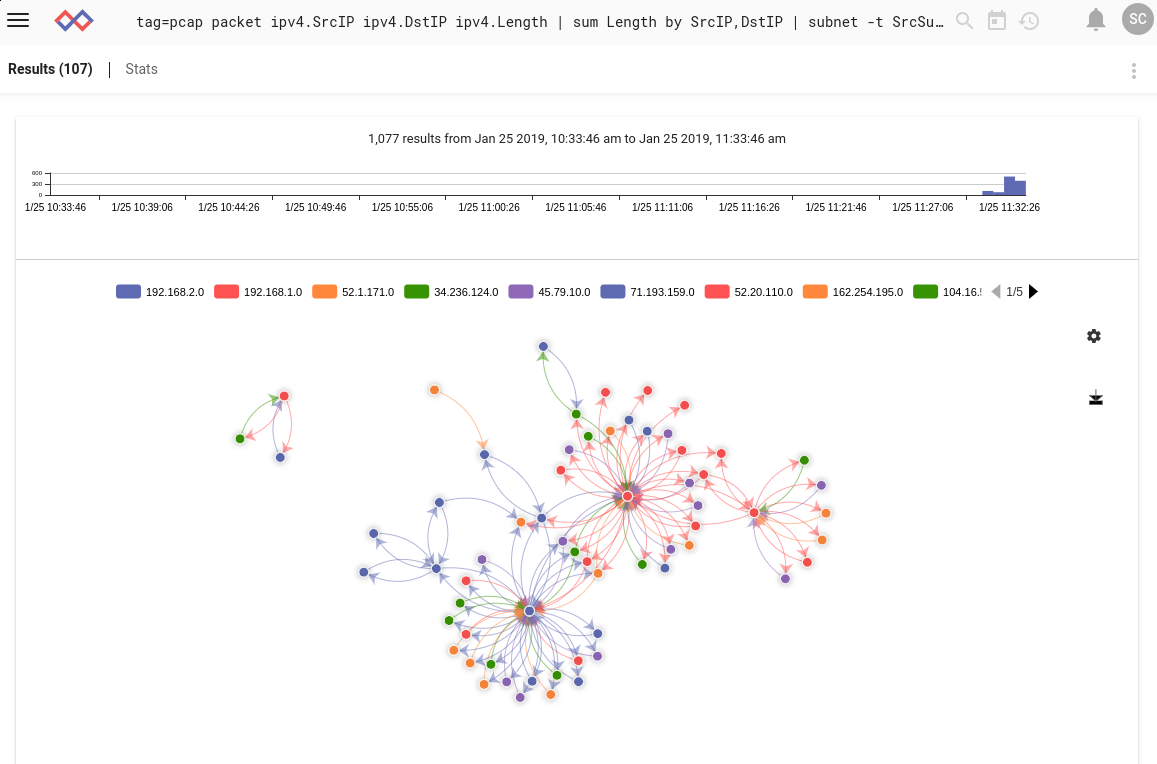
\includegraphics[width=0.6\linewidth]{images/fdg-classC.png}
	\caption{FDG of traffic between class C networks}
	\label{fig:fdg-classC}
\end{figure}

Hovering the mouse over a node shows its label and the labels of its
neighbors, as in Figure \ref{fig:fdg-context}.

\begin{figure}
	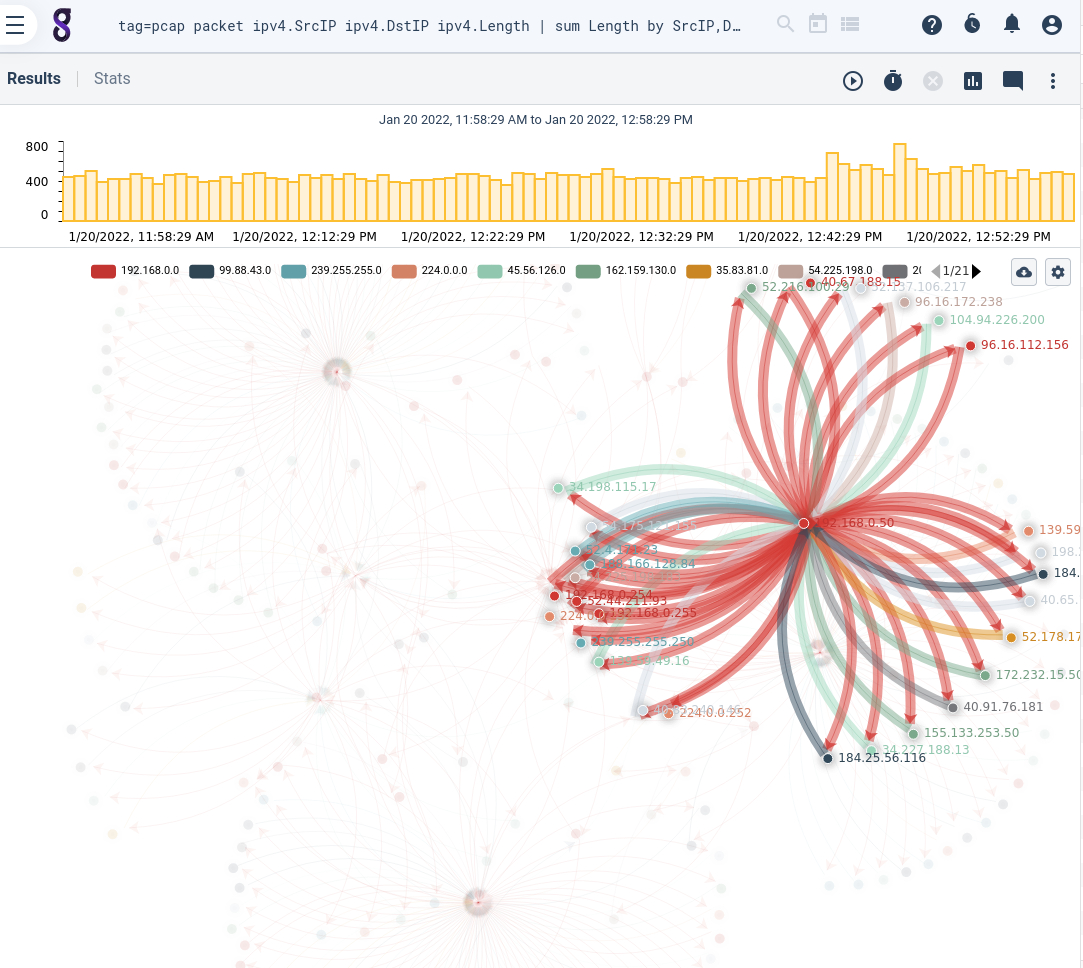
\includegraphics[width=0.6\linewidth]{images/fdg-context.png}
	\caption{FDG context popup}
	\label{fig:fdg-context}
\end{figure}

\clearpage

\section{Resources}
\label{sec:resources}
\index{Resources}
\emph{Resources} are persistent data objects which can be used in search
queries. Resources can be manually uploaded by a user or automatically
created by search modules. Resources are used by the lookup module to
store lookup tables and by the anko module to store scripts.

The format of a resource is not restricted; from the point of view of
Gravwell, a resource is simply a stream of bytes. Deriving meaning from
that stream of bytes is up to the search modules: \code{lookup} expects data in
a particular binary encoding, while \code{anko} simply treats the resource as a
text file. Scripts written for the anko module may themselves create and
access resources in a variety of formats, such as JSON-encoded text.

\subsection{Resource Basics}

Every resource is uniquely identified with a GUID, which is assigned
when the resource is created. Resources also have a human-friendly name
selected by the user. A resource can be accessed by specifying either
the GUID or the name, but be aware that names can be changed. When
building a dashboard or a search query you intend to share with others,
we recommend using the GUID to refer to the resource.

Global resources are resources created by admin-level users for access
by all users. Resources can also be shared with particular groups.

Resource data can be generated by hand or by running a search. For
example, a search that results in a table display can be downloaded in
the ``lookupdata'' format and uploaded into the resource system.

\subsection{Resource name resolution}

The resource system does not enforce unique resource names. Multiple
users can have a resource named ``foo'', or indeed one user can own
multiple resources named ``foo''. It is therefore important to be aware of
the way the resource system resolves resource names into unique GUIDs.

Consider an example invocation of an anko script in a search: \code{anko
myscript}. The resource manager will attempt to locate a resource named
``myscript'' in the following order:

\begin{itemize}
\item
  Check if the invoking user has a resource named ``myscript''; if he
  or she has multiple resources with that name, it will return the first
  match.
\item
  Check each group to which the user belongs. If there is a resource
  named ``myscript'' shared with one of the user's groups, it will
  return that resource.
\item
  Check if there is a global resource named ``myscript''.
\end{itemize}

Note that the user could be a member of groups A and B, and that there
could be one resource named myscript shared with group A and another
unique resource named myscript shared with group B; which resource
is returned is not certain. Similarly, if there are multiple global
resources named myscript, any one of them could be returned.

This ambiguity can be overcome in two ways. The safest choice is to
specify the resource as a GUID, which can be found in the resource
management page, but GUIDs are very unwieldy and provide little useful
context to the user. Luckily, it is also possible to select a resource
by name with more precision by prefixing the resource name with a
\emph{namespace}. The following are valid namespace selections:

\begin{itemize}
\item
  \code{GLOBAL:myscript} specifies a global resource named myscript.
  This will ignore any resources owned by the invoking user and go
  straight to the global resources.
\item
  \code{user=jfloren:myscript} specifies a resource named
  myscript belonging to the user jfloren. Note that this will
  fail if the invoking user does not have access to this resource.
\item
  \code{group=security:myscript} specifies a resource named
  myscript which is shared to the group ``security''. Note that this
  will fail if the invoking user is not a member of the
  ``security'' group.
\end{itemize}

\subsection{Managing resources with the GUI}

Resources are managed via a page accessible from the main menu of the user interface. Open the
menu and select "Resources" (Figure \ref{fig:resource-page}).

\begin{figure}
	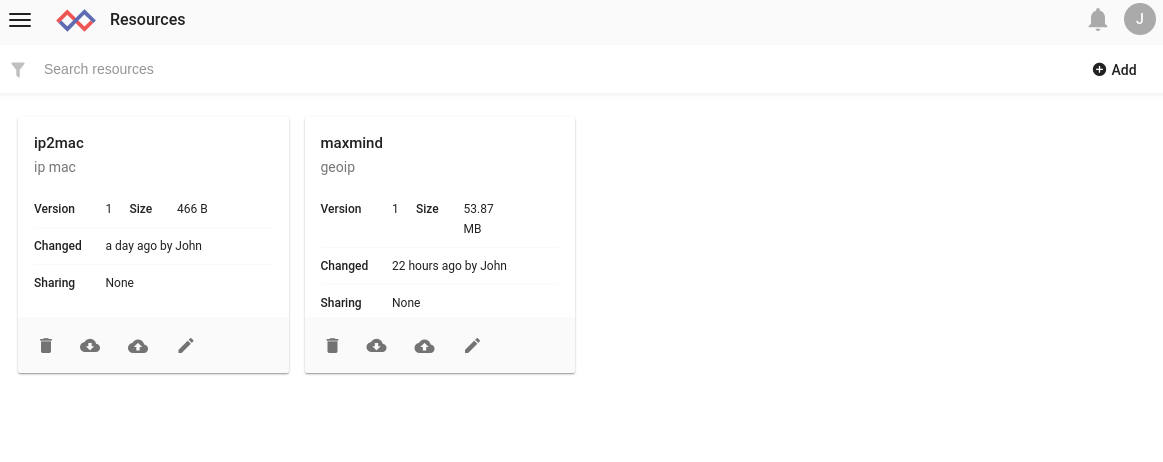
\includegraphics[width=0.7\linewidth]{images/resource-page.png}
	\caption{Resources management page}
	\label{fig:resource-page}
\end{figure}

Resources can be created and deleted from this menu.

\subsubsection{Deleting resources}

To delete an existing resource, click the trash can icon next to the
desired resource in the list. 

\subsubsection{Creating resources}

To create a new resource, select the "Add" button in the upper right. This
will open a dialog window, as shown in Figure \ref{fig:resource-new}.
Set the resource name and description as desired and select any groups
which should be able to read the resource, then select a file to upload.
Note that the resource will not be created or uploaded unless the 'Save'
button is clicked!

\begin{figure}
	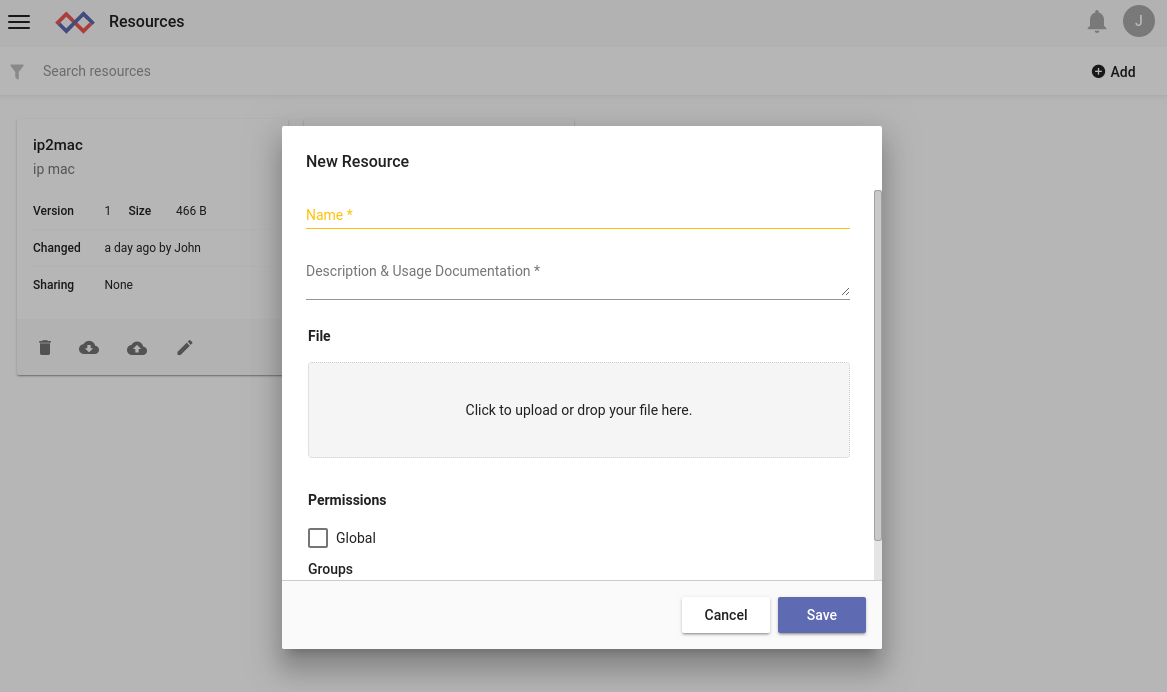
\includegraphics[width=0.7\linewidth]{images/resource-new.png}
	\caption{New resource dialog}
	\label{fig:resource-new}
\end{figure}

\subsubsection{Editing resources}

To edit an existing resource, click the pencil "Edit" icon below the
desired resource in the resource list. This will open the resource
editing screen as shown in Figure \ref{fig:resource-edit}.

\begin{figure}
	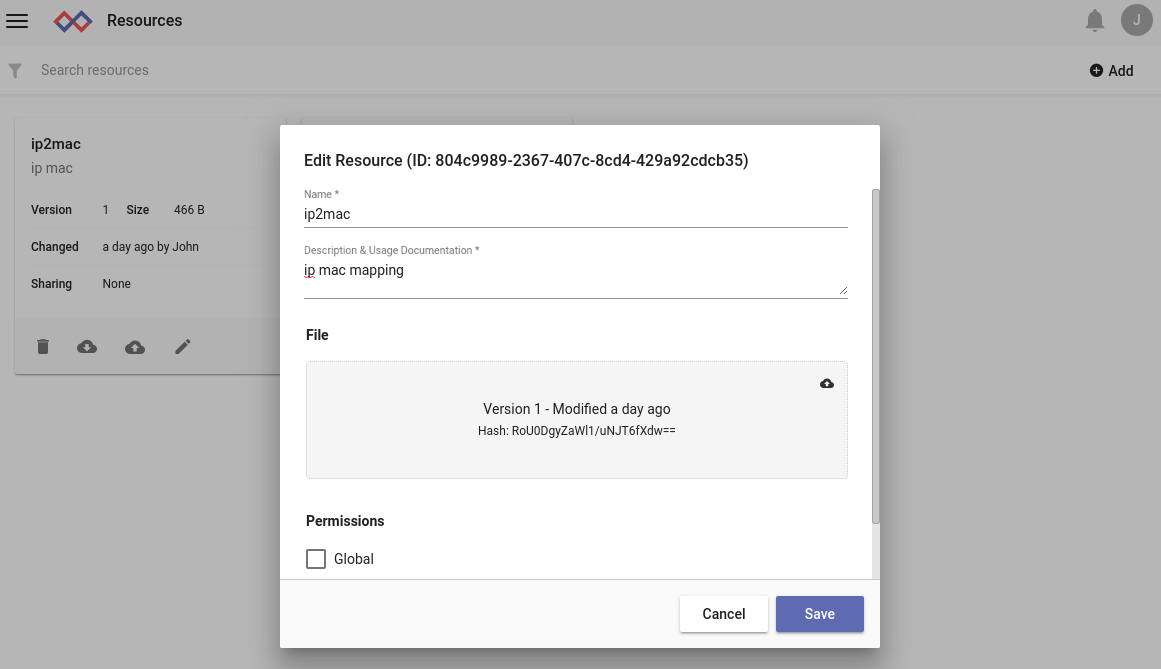
\includegraphics[width=0.7\linewidth]{images/resource-edit.png}
	\caption{Resource editing dialog}
	\label{fig:resource-edit}
\end{figure}

The name, description, and group sharing can all be managed from this
screen. Admin users can also choose to make a resource global or
non-global.

To change the actual contents of the resource, drag a file into the
grey 'File' region or click to select a new file, exactly as when
creating a new resource. Note that the Version, Hash, Size, and Last
Modified fields change when a different file is uploaded.

\clearpage
\subsection{Hands-on Lab: Enriching Netflow with GeoIP}

This lab will demonstrate how resources can be used to enrich entries
in the pipeline. We will use the geoip module to add location
information based on the source IP of each flow, then show those flows
on a map.

First, launch a Gravwell webserver+indexer container:

\begin{Verbatim}[breaklines=true]
docker run --rm --net gravnet -p 8080:80 -d --name gravwell gravwell:base
\end{Verbatim}

Next, start the ingester container running the netflow ingester:

\begin{Verbatim}[breaklines=true]
docker run --rm -d --net gravnet --name ingesters \
-e GRAVWELL_CLEARTEXT_TARGETS=gravwell:4023 \
gravwell:ingesters /opt/gravwell/bin/gravwell_netflow_capture
\end{Verbatim}

The netflow ingester is pre-configured to listen on port 2055 for
incoming Netflow v5 records.

Now, we use another Docker container to generate Netflow records and
send them to the ingester:

\begin{Verbatim}[breaklines=true]
docker run -it --net gravnet --rm \
networkstatic/nflow-generator -t ingesters -p 2055
\end{Verbatim}

The netflow generator will run indefinitely, generating flow records,
until killed.

Next we will upload a resource containing the MaxMind GeoIP database.
Go to
\href{https://dev.maxmind.com/geoip/geoip2/geolite2}{https://dev.maxmind.com/geoip/geoip2/geolite2/} and
download the ``GeoLite2 City'' database in MaxMind DB format. Unpack the file
using tar; it should contain a file named \code{GeoLite2-City.mmdb}.

Upload that file into a new resource named ``maxmind'', as shown in Figure \ref{fig:maxmind-upload}.

\begin{figure}
	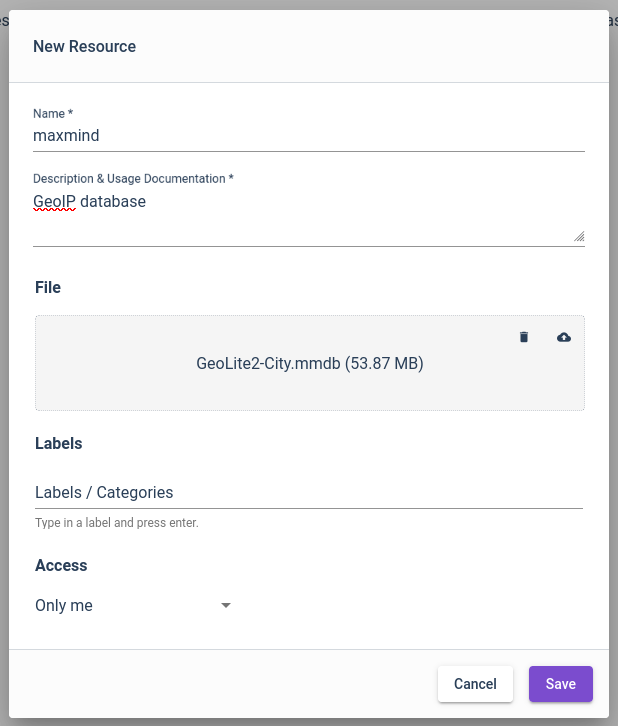
\includegraphics[width=0.5\linewidth]{images/maxmind-upload.png}
	\caption{Uploading maxmind database}
	\label{fig:maxmind-upload}
\end{figure}

With the GeoIP database uploaded, run the following query:

\begin{Verbatim}[breaklines=true]
tag=netflow netflow Src | ip Src !~ PRIVATE
| geoip -r maxmind Src.Location | pointmap Src
\end{Verbatim}

This search pulls all entries tagged ``netflow'' and hands them to the
netflow module, which extracts the Src field. The ip module is used to
eliminate Src IPs in private subnets. The geoip module then uses the
resource named ``maxmind'' to look up the Location for each Src IP
address. Finally, the pointmap renderer draws each location on a map, as
seen in Figure \ref{fig:maxmind-pointmap}.

\begin{figure}
	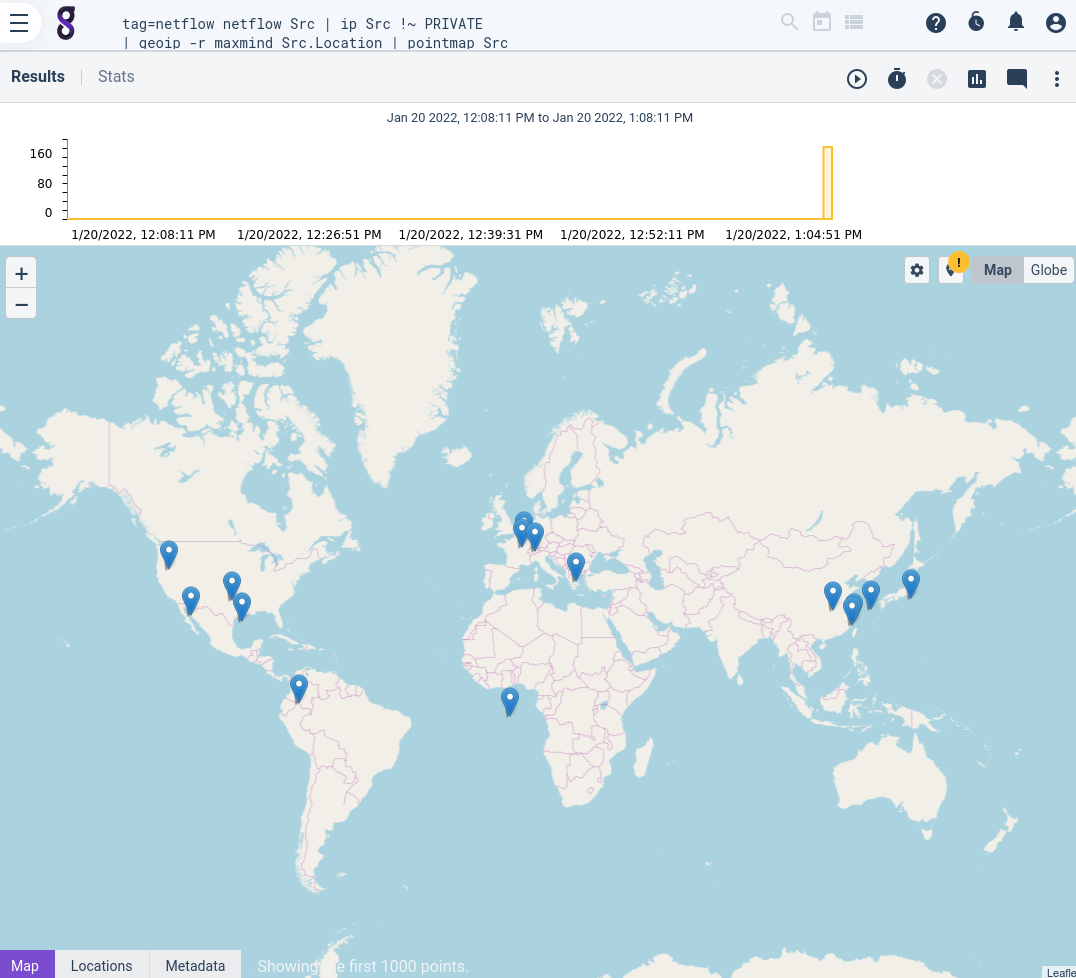
\includegraphics[width=0.7\linewidth]{images/maxmind-pointmap.png}
	\caption{Netflow source IP pointmap}
	\label{fig:maxmind-pointmap}
\end{figure}

To clean up after the experiment, simply run:

\begin{Verbatim}[breaklines=true]
docker kill $(docker ps -a -q)
\end{Verbatim}


\clearpage

\section{Data Fusion}
\index{Data fusion}\index{Search!data fusion}
The Gravwell query pipeline supports what we call module interleaving,
which is basically the ability to specify that a given module should only process
specific tags. This allows Gravwell to operate on multiple data formats
at once and optionally fuse the results into a single cohesive data
stream, essentially data fusion. Data fusion can be used to enrich one
data stream from another, provide unified visibility across multiple
data sources, or generate a single view for an operator that fuses many
different data sources.

Tags form the basis of data control in the Gravwell pipeline.
Previously we have only shown tags being used
to control what data \emph{enters} the pipeline. However, we can also add tag
specifications to individual modules and to inform them that they should
only process entries with those specific tags. Any entries that do not
match the specified tags are passed through untouched. This is what we
call data fusion.

Most data fusion queries are broken into three sections. The first section
is the extraction phase where we use the data bypass and additional
tag specifications to target modules against specific data types,
for example we might have an unstructured log and JSON data. We use
the tags to invoke the json module against the JSON data and the regex
module against the unstructured data. The next section of a fusion query
might use one data source to enrich or pivot on the other, potentially
creating a running lookup system that adds additional enumerated values
to one tag but derived from the other. The final section tends to look like
regular search pipelines, using the data fused data without targeting any particular tag.

The following diagram shows what a data fusing query might look like.
We have two data sources coming in, let's call them tag RED and tag
BLUE. There are three modules that have been instructed to only
operate on either RED or BLUE data, then there is a fusing
module (orange) that uses the RED and BLUE data to create a
single data stream with both data types fused. The final search module
performs some standard operation on \emph{all} entries before sending the data on to the
renderer.

\begin{figure}
	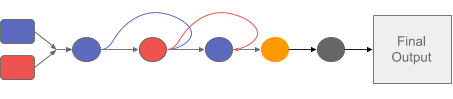
\includegraphics{images/data-fusion-pipeline.png}
	\caption{Data fusion notional pipeline}
	\label{fig:data-fusion-pipeline}
\end{figure}

Let's look at an example query that represents this diagram. We have
color coded the search module statements to help associate them with the
diagram:

%%% I apologize for this nasty-looking code, it's the only way I know to get colors in
\code{tag=\textcolor{red}{RED},\textcolor{blue}{BLUE tag=BLUE json X Y} \\
\textbar{} \textcolor{red}{tag=RED regex ``(?P\textless{}B\textgreater{}\textbackslash{}S+)\textbackslash{}s(?P\textless{}X\textgreater{}\textbackslash{}S+)\textbackslash{}s''} \\
\textbar{} \textcolor{blue}{tag=BLUE regex -e X ``[\^\textbackslash{}.]+\textbackslash{}.(?P\textless{}B\textgreater{}.+)''} \\
\textbar{} \textcolor{orange}{stats sum(X) variance(Y) by B} \\
\textbar{} sort by sum desc \\
\textbar{} table sum variance B}

Data fusion queries that perform enrichment will often need the
\code{eval} module and persistent maps in order to save enumerated values
from one entry and attach them to another. Here is the same query but
instead of generating a unified set of stats using the two sources, we
are going to enrich the RED data with the BLUE data:

\code{tag=\textcolor{red}{RED},\textcolor{blue}{BLUE tag=BLUE json X Y} \\
\textbar{} \textcolor{red}{tag=RED regex ``(?P\textless{}B\textgreater{}\textbackslash{}S+)\textbackslash{}s(?P\textless{}X\textgreater{}\textbackslash{}S+)\textbackslash{}s''} \\
\textbar{} \textcolor{orange}{eval if(TAG==BLUE)\{ \\
setPersistentMap(``X'', X, Y); \\
~~~~return false \\
\} else \{ \\
~~~~setEnum(``Y'', getPersistentMap(``X'', X)) \\
\}} \\
\textbar{} table B X Y}

This query looks daunting, but it is not terribly complicated. We have
the RED and BLUE data streams coming in, each of which is processed by a
different search module to extract data. Then the eval module will
either save a key/value pair or lookup a key/value pair depending on the
tag. For this example, if the entry has a BLUE tag we are saving the Y
value with a key of X, then we drop the entry. If the tag is not
BLUE (translation: the tag is RED) then we attempt to look up the X key in the map and assign
the result into the enumerated value ``Y''. The output is a single data stream
that essentially unifies the RED and BLUE data sets using a common key
B.

\clearpage
\subsection{Hands-on Lab: Data Fusion}

For this lab we are going to be fusing data from three different
sources: dhcp server logs and switch logs. The end result will be a
single table that shows computers with their MAC address, IP address,
hostname, and switch port. An admin can use this query to identify a
machine by name and see the switch port is connected to, all in a single
query. Let's start by ingesting our dataset and building extractions
that pull the appropriate data from each tag. We will be using the
tags ``dhcp'' and ``switch''.

Note that this lab is one of the most challenging in this training document. It makes use of the powerful but complex regex (\href{https://docs.gravwell.io/\#!search/regex/regex.md}{https://docs.gravwell.io/\#!search/regex/regex.md}) and eval (\href{https://docs.gravwell.io/\#!search/eval/eval.md}{https://docs.gravwell.io/\#!search/eval/eval.md}) modules. We recommend carefully reading the examples shown in the lab instructions and those in the preceding section; these should demonstrate any necessary invocations of the modules. We also recommend using \href{https://regex101.com/}{https://regex101.com/} to help build and test regular expressions if needed.

First, we'll start the Gravwell container:

\begin{Verbatim}[breaklines=true]
docker run --rm --net gravnet -p 8080:80 -d --name gravwell gravwell:base
\end{Verbatim}

Then we'll ingest the data, found in the \code{gravwell\_training/Search/Lab-Fusion} subdirectory:

\begin{Verbatim}[breaklines=true]
cd ~/gravwell_training/Search/Lab-Fusion

docker run -v $PWD/data:/tmp/data --rm -i --net gravnet \
gravwell:ingesters /opt/gravwell/bin/reimport -rebase-timestamp \
-clear-conns gravwell:4023 -i /tmp/data/dhcp.json.gz -import-format json

docker run -v $PWD/data:/tmp/data --rm -i --net gravnet \
gravwell:ingesters /opt/gravwell/bin/reimport -rebase-timestamp \
-clear-conns gravwell:4023 -i /tmp/data/switch.json.gz -import-format json
\end{Verbatim}

Let's look at the switch tag first. Here is an example entry:

\begin{Verbatim}[breaklines=true]
<135>2019-03-22 20:20:24 192.168.0.100 71565 The switch has learned a new
MAC address 50:2e:5c:e5:46:0b, vid:1024, interface:port 13
\end{Verbatim}

We want to extract the MAC address (50:2e:5c:e5:46:0b) and switch
port (13). Let's use the following regular expression:

\begin{Verbatim}[breaklines=true]
(?P<mac>[\da-f:]+),\s\S+\sinterface:port\s(?P<port>\d+)
\end{Verbatim}

Test your regular expression by running the query:

\begin{Verbatim}[breaklines=true]
tag=switch grep "new MAC address"
| regex "(?P<mac>[\da-f:]+),\s\S+\sinterface:port\s(?P<port>\d+)"
| table mac port
\end{Verbatim}

Next let's extract our hostnames from the DHCP log. Here is an example
entry where a client ACKs a DHCP lease; it contains the hostname,
IP, and MAC address:

\begin{Verbatim}[breaklines=true]
<30>1 2019-07-08T23:59:22.417203-06:00 router dhcpd 12365 - - 
DHCPACK on 10.10.10.10 to e8:94:f6:1a:2b:c5 (keg) via insecure
\end{Verbatim}

Let's use the following regular expression to extract the IP, MAC, and
potentially a hostname:

\begin{Verbatim}[breaklines=true]
\s(?P<ip>[\d\.]+) to (?P<mac>[\da-f:]+)(\s\((?P<host>\S+)\))?
\end{Verbatim}


Test the regular expression with:

\begin{Verbatim}[breaklines=true]
tag=dhcp grep "ACK on " 
| regex  "\s(?P<ip>[\d\.]+) to (?P<mac>[\da-f:]+)(\s\((?P<host>\S+)\))?"
| table mac ip host
\end{Verbatim}

We now have the ability to extract all the relevant pieces from our
tags, let's start combining them starting with the switch and
dhcp tags. Let's look at a query that uses both tags to create a
single data stream with ip, mac address, and switch port:

\begin{Verbatim}[breaklines=true]
tag=switch,dhcp
tag=switch grep "new MAC address" 
| tag=dhcp grep "ACK on " 
| tag=dhcp regex "\s(?P<ip>[\d\.]+) to (?P<mac>[\da-f:]+)(\s\((?P<host>\S+)\))?"
| tag=switch regex "(?P<mac>[\da-f:]+),\s\S+\sinterface:port\s(?P<port>\d+)"
| table mac host port TAG
\end{Verbatim}

This should create a table that shows the extracted values for each
tag. Now let's use eval to enrich the dhcp logs with the switch logs:

\begin{Verbatim}[breaklines=true]
tag=switch,dhcp tag=switch grep "new MAC address"
| tag=dhcp grep "ACK on "
| tag=dhcp regex "\s(?P<ip>[\d\.]+) to (?P<mac>[\da-f:]+)(\s\((?P<host>\S+)\))?"
| tag=switch regex "(?P<mac>[\da-f:]+),\s\S+\sinterface:port\s(?P<port>\d+)"
| sort by time asc
| eval if(TAG=="switch"){ setPersistentMap("ports", mac, port)
} else { setEnum("port", getPersistentMap("ports", mac)) }
| eval TAG=="dhcp" 
| require port 
| unique mac host port 
| table mac host port
\end{Verbatim}

The eval logic is a boolean if/else statement that sets the port value
using the MAC as key if the tag is ``switch'', and looks up the port using the
MAC key if not. Another eval statement drops all entries that are not
tagged ``dhcp''. We then unique the list and generate a table. Here is the eval
logic formatted a little better:

\begin{Verbatim}[breaklines=true]
if(TAG=="switch") {
    setPersistentMap("ports", mac, port)
} else {
    setEnum("port", getPersistentMap("ports", mac))
}
\end{Verbatim}

Make note of the additional \code{sort by time asc} search module.  Gravwell
loosely orders data by time when executing queries, but correlations like
DHCP and switch actions are operating on data where microseconds matter,
so it is important to strictly order the data by time in the pipeline
so that the switch logs occur before the DHCP logs so that a mac address
from the DHCP log can be looked up against a MAC address from the switch log.

\begin{figure}
	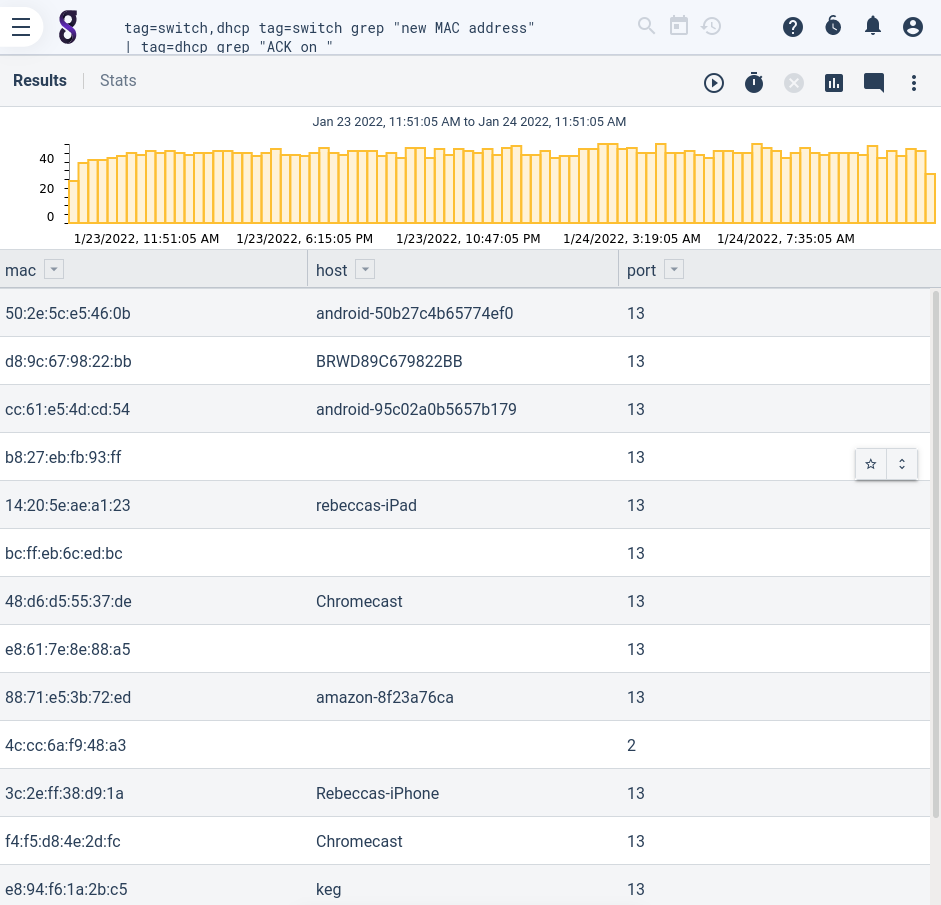
\includegraphics[width=0.6\linewidth]{images/mac-host-table.png}
	\caption{MAC / Hostname / Switch Port table}
	\label{fig:mac-host-table}
\end{figure}

The resulting table (Figure \ref{fig:mac-host-table}) is pretty useful for keeping an eye on what devices are on your network. Note that some MAC addresses don't have a hostname associated with them; those are devices we may want to investigate!

\subsubsection{Lab Tasks}

\begin{enumerate}
\item
  Try adapting the query to also extract the vlan id (vid) from the
  switch logs and add it to the table.
\item
  Adapt the query to set the hostname to ``UNKNOWN'' if the DHCP log
  doesn't have a hostname
\item
  Generate an FDG with host to vid
\item
  Can you find any hosts on more than one vlan?
\end{enumerate}

\begin{samepage}
\subsubsection{Lab Questions}
\begin{enumerate}
\item
  {When would data fusion enrichment make more sense than creating a
  resource and using lookup?}
\item
  {When would data fusion not work}
\item
  {How would you combine the two methods to get ``the best of both
  worlds''?}
\end{enumerate}
\end{samepage}

To clean up after the experiment, simply run:

\begin{Verbatim}[breaklines=true]
docker kill $(docker ps -a -q)
\end{Verbatim}

\section{Query Optimization}
\label{sec:query-optimization}
\index{Search!optimization}
The Gravwell query pipeline is very powerful. Searches are distributed
to all nodes in the cluster, who intelligently share the load in order to
maximize computing resources at top efficiency. It is possible, however,
to issue searches in a way that degrades or hampers this.
This section describes module ordering, condensing modules, and filtering
and how to avoid common pitfalls.

For purposes of discussion, we are going to break modules
down into three categories: parsers, operators, and condensers. Render
modules are not a consideration when it comes to optimization, as they
are always the final module in a pipeline.
\index{Search!modules}

\subsection{Parsing modules}
A parsing module is one that performs field extraction over a data
entry. Typically, these modules are slower than operating modules as
they usually read and process the entire data entry and create
enumerated values for any given fields. The \code{json} module, as an
example, will parse an entire JSON record and create enumerated values
as directed.

For example, say we had some very large JSON entry that looked like:

\begin{Verbatim}[breaklines=true]
{ ‘field1’: ‘a’, ‘field2’: ‘aa’, ‘field3’: ‘aaa’, ‘field4’: ‘aaaa’, 
… ‘field8000’: ‘aaaaaaaaaaaaaaaaaa....}
\end{Verbatim}

If we ran a search like \code{json field2 field488 field8000}, the json
module would have to read and parse the entirety of the record. Gravwell
distributes these parsing modules to every indexer in the cluster and
these are run very close to the data.

\subsection{Parsing modules and Accelerators}
\index{Acceleration}
Accelerators are covered in Section \ref{sec:acceleration} and in the online
Gravwell documentation, but they should be mentioned when discussing query optimization.
When turned on, they provide very powerful filtering speedups using our hybrid
indexing technology. Invocation of those accelerators occurs in the
parsing modules. In the case of no accelerators being present, filtering
arguments that are provided in parsing modules are invoked after the
parsing has occurred.

Using the above example, if we had accelerators turned on for ``field3''
and issued a search like: \code{json field3=="foo"}, this would invoke the
accelerator framework to perform filtering before parsing of JSON is
necessary. In this case, that parsing was done ahead of time by the
accelerator and an index was created for rapid lookup.

In general, it is desirable to do field-based filtering in the parsing
module, as it can engage acceleration if available.

\subsection{Operator modules}

For purposes of discussing optimization, operator modules are the
common `bread and butter' search modules available for the Gravwell
search pipeline. They run in parallel close to source data (i.e. on
the indexers). These modules are what do the filtering, extracting,
enriching, and other analysis to be used further down the pipeline.

Note: Operator modules in pipeline \emph{after} a condensing module will
execute in series on the Gravwell webserver frontend.

\subsection{Condenser modules}

Condensing modules are those modules which require \emph{all} of the data to
be present. These modules trigger a collapse of the pipeline from a
parallel series running on the indexers to a single pipeline running on
the Gravwell webserver. These are the modules that do counting, sum
fields, strip non-unique values, etc. They require the entirety of data
to be present in order to provide accurate results.

These modules are all of the \href{https://docs.gravwell.io/\#!search/math/math.md}{math
modules}(count, sum, max, etc),
\href{https://docs.gravwell.io/\#!search/stats/stats.md}{stats},
\href{https://docs.gravwell.io/\#!search/anko/anko.md}{anko}, and
\href{https://docs.gravwell.io/\#!search/eval/eval.md}{eval}.

Let's use the query \code{json field1 \textbar{} stats max(field1)} as an
example where we are looking to find the maximum value of field1 in our
data. When a collapse occurs, the indexers perform the analysis on what
data they possess first, and then send the data to the Gravwell
webserver to be aggregated in total.

Any modules following a condensing module will then be operating in
series on the webserver, not in parallel on the indexers.

\clearpage
\subsection{Hands-on Lab: Optimizing Queries}

Let's look at a few searches that all accomplishing the same end
results of filtering and analyzing some JSON data. We will execute these
queries within the lab docker environments, but the differences won't be
as noticeable on such a small scale. For any Gravwell deployment with
significant data or node count, however, the knowledge in this section
is invaluable.

We need to fire up the base Gravwell container and then the ingesters
container to generate some sample JSON entries:

\begin{Verbatim}[breaklines=true]
docker run --rm --net gravnet -p 8080:80 -d --name gravwell gravwell:base

docker run --net gravnet --rm -it --name jsoningesters gravwell:ingesters\
 /opt/gravwell/bin/jsonGenerator -clear-conns gravwell:4023 -entry-count 100000
\end{Verbatim}

Let's begin by examining the data:

\begin{Verbatim}
tag=json
\end{Verbatim}

Here is an example of the data we're looking at:

\begin{Verbatim}[breaklines=true]
{
   "time":"2022-06-09T13:03:36Z",
   "account":{
      "user":"jacobbrown802",
      "name":"Jacob Jones",
      "email":"jacobbrown802@example.org",
      "phone":"+850 169 94 122 338",
      "address":"58 Adams Circle, Ransom Canyon, PW, 97213",
      "state":"AZ",
      "country":"Netherlands Antilles"},
   "class":43294,
   "groups":["mouse","falcon"],
   "user_agent":"Mozilla/5.0 (Windows NT 6.3; Trident/7.0; rv:11.0) like Gecko",
   "ip":"102.115.187.35",
   "data":"One dog rolled before him, well-nigh slashed in half; but a second had him by the thigh, a third gripped his collar be- hind, and a fourth had the blade of the sword between its teeth, tasting its own blood."
}
\end{Verbatim}

The data generated is random. To complete this lab, examine the entries and make note of values found for user\_agent, groups, and some random words found in data.
For example, in our sample entry above, we may note the following:
\begin{itemize}
\item user\_agent
\subitem "Mozilla/5.0 (Windows NT 6.3; Trident/7.0; rv:11.0) like Gecko"
\item groups
\subitem "mouse"
\subitem "falcon"
\item random words found in data
\subitem "dog"
\subitem "collar"
\subitem "sword"
\end{itemize}

In the searches below, make replacements using your pre-selected values.

Let's start with the base search that's looking to see how many entries
for each group except 'mouse' have a specific user agent we are
investigating and are not talking about a dog.

\begin{Verbatim}[breaklines=true]
tag=json json -x groups groups account.user account.email ip data class user_agent 
| eval user_agent=="Mozilla/5.0 (Windows NT 6.3; Trident/7.0; rv:11.0) like Gecko" 
| grep -e data -v "[dD]og" | stats count by groups | grep -v -e groups "mouse" | table groups count
\end{Verbatim}

That query invokes a parsing module and then immediately condenses with
an eval module that's inefficiently being used to match the user agent.
We can improve this query by moving the user agent match into the
parsing module:

\begin{Verbatim}[breaklines=true]
tag=json json -x groups groups account.user account.email ip data class 
user_agent=="Mozilla/5.0 (Windows NT 6.3; Trident/7.0; rv:11.0) like Gecko" 
| grep -e data -v "[dD]og" | stats count by groups | grep -v -e groups "mouse" | table groups count
\end{Verbatim}

This query is also performing the check to remove the 'mouse' group
after the pipeline has condensed. This filtering can also be moved into
the parser module:

\begin{Verbatim}[breaklines=true]
tag=json json -x groups groups!="mouse" account.user account.email ip data class 
user_agent=="Mozilla/5.0 (Windows NT 6.3; Trident/7.0; rv:11.0) like Gecko" 
| grep -e data -v "[dD]og" | stats count by groups | table groups count
\end{Verbatim}

This is looking a lot better but, depending on whether or not we have
accelerators enabled for the various fields of this data, we can
possibly improve the query even further. If accelerators are NOT
enabled, it is actually more performant to do basic matching \emph{before} the
parsing module. The \code{grep} module is the fastest filtering module in the
Gravwell pipeline when operating on the raw data entries. Let's improve
further:

\begin{Verbatim}[breaklines=true]
tag=json grep "Mozilla/5.0 (Windows NT 6.3; Trident/7.0; rv:11.0) like Gecko" 
| json -x groups groups!="mouse" account.user account.email ip data class user_agent
| grep -e data -v "[dD]og" | stats count by groups | table groups count
\end{Verbatim}

We have optimized the query but beware, as this query now has
potential to produce unintended results. If the data section of these
log entries were to contain this \code{user\_agent} string (perhaps a user is
posting a message requesting technical support), then that entry would
match the initial grep despite having an incorrect user agent. Thus, to
further optimize for performance (and not for query length), we can put
the filter back in the parsing module to ensure correctness of results:

\begin{Verbatim}[breaklines=true]
tag=json grep "Mozilla/5.0 (Windows NT 6.3; Trident/7.0; rv:11.0) like Gecko" 
| json -x groups groups!="mouse" account.user account.email ip data class 
user_agent=="Mozilla/5.0 (Windows NT 6.3; Trident/7.0; rv:11.0) like Gecko"
| grep -e data -v "[dD]og" | stats count by groups | table groups count
\end{Verbatim}

Something to keep in mind is that if accelerators \emph{are} enabled, then the
initial grep would be a detriment to performance. See section \ref{sec:acceleration} for additional
details on query acceleration.

As an exercise, try and sort the above queries from worst to best by
writing numbers in the margins. On the left margin, put the number
ranking in a scenario where accelerators are disabled. On the right
margin, put the number ranking where they are enabled.

To clean up after the experiment, simply run:

\begin{Verbatim}[breaklines=true]
docker kill $(docker ps -a -q)
\end{Verbatim}





\section{Auto-extractors}
\index{Search!extractors}\index{Auto-extractors|see {Extractors}}\index{Extractors}
Gravwell enables per-tag extraction definitions that can ease the
complexity of interacting with unstructured data and data formats that
are not self-describing. Unstructured data often requires complicated
regular expressions or slice specifications to extract desired data
fields, which can be time-consuming to produce and prone to errors.

Auto-extractors are simply definitions that can be applied to tags which
describe how to correctly extract fields from the data in a given tag.
The "ax" module then automatically invokes the appropriate functionality
of other modules. The auto-extractor system supports the following
extraction methods:

\begin{itemize}
\tightlist
\item
  CSV
\item
  Fields
\item
  Regex
\item
  Slice
\item
  KV
\item
  Syslog
\item
  JSON
\item
  Grok
\item
  CEF
\end{itemize}

Auto-extractor definitions are used by
the \href{https://docs.gravwell.io/\#!search/ax/ax.md}{ax} module
which transparently references the correct extraction based on tags.

Note that only a single extraction can be defined per tag per user. Also note
that auto-extractors always operate on the full underlying data of an
entry. They cannot be used to perform extractions on Enumerated Values
(the "-e" argument is disallowed)

\subsection{Auto-Extractor Configuration}

Every auto-extractor can define the following parameters:

\begin{itemize}
\item
  tag - The tag associated with the extraction
\item
  name - A human-friendly name for the extraction
\item
  desc - A human-friendly string that describes the extraction
\item
  module - The processing module used for extraction (regex, slice,
  csv, fields, etc.)
\item
  args - Module-specific arguments used to change the behavior of the
  extraction module
\item
  params - The extraction definition
\end{itemize}

Only the module, params, and tag parameters are required;
all others can be left blank if desired (for example, the regex module
does not take any arguments, so args will always be empty).

\subsection{Managing Auto-Extractors in the GUI}
\index{GUI!extractors}
The Gravwell GUI can be used to manage extractors. The screenshot in Figure \ref{fig:extractors-page}
shows the Extractors page with four defined extractors.

\begin{figure}
	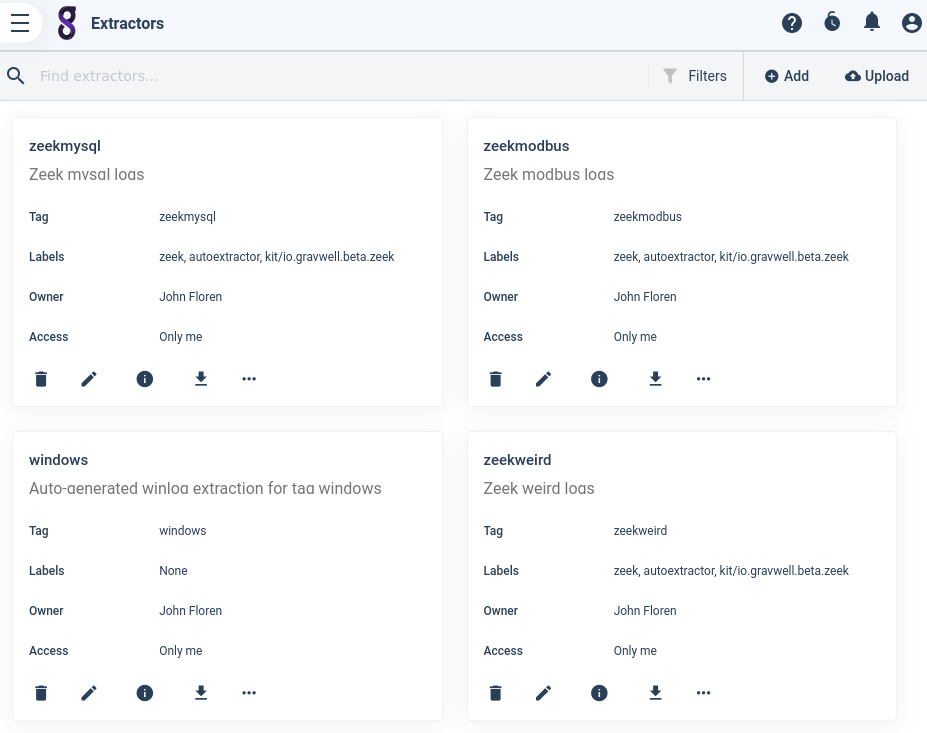
\includegraphics[width=0.7\linewidth]{images/extractors-page.png}
	\caption{Extractors page}
	\label{fig:extractors-page}
\end{figure}

Note the buttons in the upper right. ``Add'' creates a new extractor
interactively, allowing the user to enter appropriate values, as seen in Figure \ref{fig:new-extractor}.

\begin{figure}
	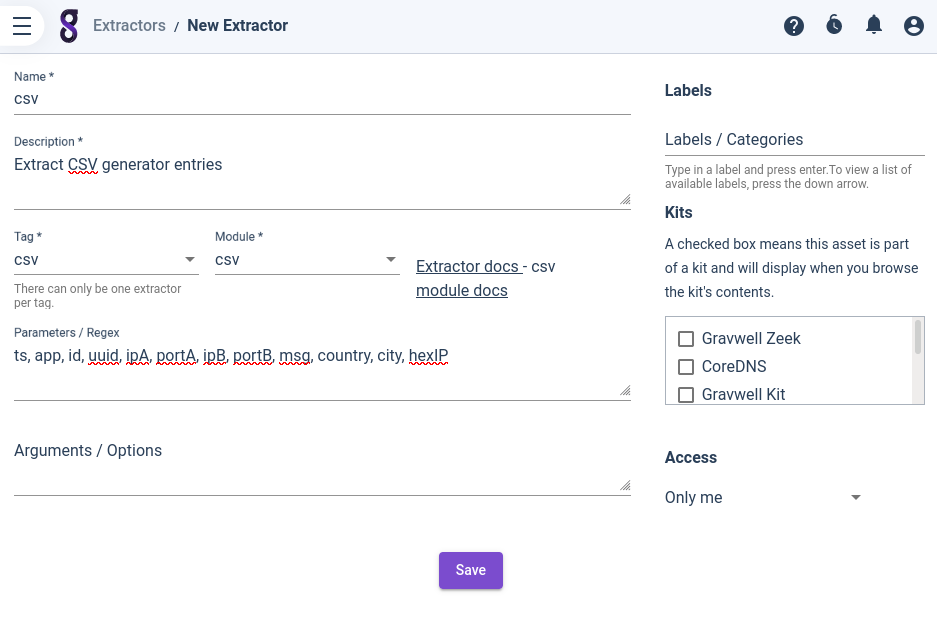
\includegraphics[width=0.7\linewidth]{images/new-extractor.png}
	\caption{New extractor dialog}
	\label{fig:new-extractor}
\end{figure}

``Upload'' allows you to directly upload files containing text versions of AX definitions; this is a convenient way to install many extractors at once.

\subsection{Auto-Extractor Files}

Auto-extractors can be defined in text files, which may then be uploaded through
the web interface. Auto-extractor files follow the TOML V4 format which allows comments
using the "\#" character. Each "ax" file can contain multiple
auto-extraction definitions.

There are a few important rules about how the extraction parameters are
defined in files:

\begin{enumerate}
\tightlist
\item
  Each extraction parameter's value must be defined as a string and
  double- or single-quoted.
\item
  Double-quoted strings are subject to string escape rules (pay
  attention when using regex), e.g. "\textbackslash{}b" would be the backspace character (character 0x08)
  not the literal string "\textbackslash{}b".
\item
  Single quoted strings are raw and not subjected to string escape
  rules, meaning '\textbackslash{}b' is literally the backslash character followed
  by the 'b' character, not a backspace.
\end{enumerate}

The ability to ignore string escape rules is especially handy for the
"regex" processor as it makes heavy use of backslash.

Here is a sample auto-extraction file designed to pull some basic data
from an Apache 2.0 access log using the regex module:

\begin{Verbatim}[breaklines=true]
#pull ip, method, url, proto, and status from apache access logs
[[extraction]]
tag="apache"
name="apacheaccess"
desc="Apache 2.0 access log extraction to pull requester items"
module="regex"
args=""
params='^(?P<ip>\d+\.\d+\.\d+\.\d+)[^\"]+\"(?P<method>\S+)\s
(?P<url>\S+)\s(?P<proto>\S+)\"\s(?P<status>\d+)'
\end{Verbatim}

Multiple extractions can be specified in a single file by simply
establishing a new \code{[[extraction]]} header and a new
specification. Defining multiple extractions in one file is a convenient
way to manage and share extractions across multiple Gravwell installations.

\subsection{Extractor Examples}

We will demonstrate a few auto-extraction definitions and compare and
contrast queries which accomplish the same task with and without
auto-extractors. We will also show how to use filters within AX.

In these examples, we show extractor definitions in the TOML file format
described above; to instantiate them through the GUI, simply save them as a file and use the Upload button.

\subsubsection{CSV}

CSV or "Comma Separated Values" can be a relatively efficient text
transport and storage system. However, CSV data is not self-describing,
meaning that if all we have is a bunch of CSV data it can be difficult
to tell what columns actually are. Auto-extractors can be used to
predefine column names and make it dramatically easier to work with CSV
data.

Here is an example data entry that is encoded using CSV:

\begin{Verbatim}[breaklines=true]
2019-02-07T10:52:49.741926-07:00,fuschia,275,
68d04d32-6ea1-453f-886b-fe87d3d0e0fe,174.74.125.81,58579,
191.17.155.8,1406,"It is no doubt an optimistic enterprise.",
"TL",Bury,396632323a643862633a653733343a643166383a643762333a
\end{Verbatim}

There is a lot of data in there with no indication of which fields are
what. To make matters worse, CSV data can contain commas and surrounding
spaces which makes identifying columns with the naked eye very
difficult. Auto-extractors allow the administrator (or user) to identify column
names and types \emph{once}; once defined, users can transparently leverage
them using the ``ax'' module.

The following query manually extracts and names each element:

\begin{Verbatim}[breaklines=true]
tag=csvdata csv [0] as ts [1] as name [2] as id [3] as guid [4] as src 
[5] as srcport [6] as dst [7] as dstport [8] as data [9] as country 
[10] as city [11] as hash
| table
\end{Verbatim}

With the following auto-extractor configuration installed:

\begin{Verbatim}[breaklines=true]
[[extraction]]
  name="testcsv"
  desc="CSV auto-extraction for the super ugly CSV data"
  module="csv"
  tag="csvdata"
  params="ts, name, id, guid, src, srcport, dst, dstport, data, country, city, hash"
\end{Verbatim}

That same query becomes:

\begin{Verbatim}[breaklines=true]
tag=csvdata ax | table
\end{Verbatim}

Note: The CSV auto-extraction processor does not support any
arguments. The position of the names in the params variable indicates
the field name. Treat it as a CSV header.

\subsubsection{Fields}

The fields module is an extremely flexible processing module that can
define arbitrary delimiters and field rules in order to extract data.
Many popular security applications like Bro/Zeek default to TSV (tab
separated values) for data export. Other custom applications may use
weird separators like ``\textbar{}'' or a series of bytes like ``//''. The
fields extractor can handle them all, and when combined with
auto-extractors users don't have to worry about the details of the data
format.

Unlike other auto-extractor processors, the fields module has a variety
of configuration arguments. The list of arguments is fully documented in
the fields module documentation. Only the ``-e'' flag is unsupported.

First, consider this tab delimited entry (line-wrapped in this document for readability):

\begin{Verbatim}[breaklines=true]
2019-02-07T11:27:14.308769-07:00    green    21.41.53.11    1212    
57.27.200.146    40348    Have I come to Utopia to hear this sort of thing?
\end{Verbatim}

Using the fields module to extract each data item, the query would be:

\begin{Verbatim}[breaklines=true]
tag=tabfields fields -d "\t" [0] as ts [1] as app [2] as src [3] as srcport
[4] as dst [5] as dstport [6] as data
| table
\end{Verbatim}

An auto-extraction configuration to accomplish the same thing is:

\begin{Verbatim}[breaklines=true]
[[extraction]]
    tag="tagfields"
    name="tabfields"
    desc="Tab delimited fields"
    module="fields"
    args='-d "\t"'
    params="ts, app, src, srcport, dst, dstport, data"
\end{Verbatim}

Using the ax module and the configuration above, the query becomes:

\code{tag=tagfields ax \textbar{} table}

The following entry uses the more unusual ``\textbar{}'' separator:

\begin{Verbatim}[breaklines=true]
2019-02-07T11:57:24.230578-07:00|brave|164.5.0.239|1212|
179.15.183.3|40348|"In C the OR operator is ||."
\end{Verbatim}

Note that the last field contains the delimiter. The system that
generated this data knew that it needed to include the delimiter in a
data item, so it encapsulated that data item in double quotes. The
fields module knows how to deal with quoted data; specifying the ``-q''
flag will make the module respect quoted fields. The quotes are kept on
the extracted data unless the ``-clean'' flag is also specified.

Using the fields search module alone, the query would be:

\begin{Verbatim}[breaklines=true]
tag=barfields fields -d "|" -q -clean [0] as ts [1] as app 
[2] as src [3] as srcport [4] as dst [5] as dstport [6] as data
| table
\end{Verbatim}

But with an appropriate auto-extraction configuration (shown below) the
query can still be the extremely simple \code{tag=barfields ax \textbar{} table}:

\begin{Verbatim}[breaklines=true]
[[extraction]]
    tag="barfields"
    name="barfields"
    desc="bar | delimited fields with quotes and cleaning"
    module="fields"
    args='-d "|" -q -clean'
    params="ts, app, src, srcport, dst, dstport, data"
\end{Verbatim}

\subsubsection{Regex}

Regex may be the most common use for auto-extractors. Regular
expressions are hard to get right, easy to mistype, and difficult to
optimize. Defining an auto-extractor allows the Gravwell administrator
to define a regex once and take the burden off the users.

Here is an example entry with a very chaotic format (which is not
uncommon in custom application logs):

\begin{Verbatim}[breaklines=true]
2019-02-06T16:57:52.826388-07:00 [fir] <6f21dc22-9fd6-41ee-ae72-a4a6ea8df767> 
783b:926c:f019:5de1:b4e0:9b1a:c777:7bea 4462 c34c:2e88:e508:55bf:553b:daa8:59b9:2715 
557 /White/Alexander/Abigail/leg.en-BZ Mozilla/5.0 (Linux; Android 8.0.0; 
Pixel XL Build/OPR6.170623.012) AppleWebKit/537.36 (KHTML, like Gecko) 
Chrome/60.0.3112.107 Mobile Safari/537.36 {natalieanderson001@test.org}
\end{Verbatim}

The data is a really ugly access log for some custom application. The
components of the entry are:

\begin{itemize}
\tightlist
\item
  {ts - the timestamp at the beginning of each entry}
\item
  {app - a string representing the handling application}
\item
  {uuid - a unique identifier}
\item
  {src - source address, both IPv4 and IPv6}
\item
  {srcport - source port}
\item
  {dst}{~- destination address, both IPv4 and IPv6}
\item
  {dstport - destination port}
\item
  {path - URL like path}
\item
  {user\_agent - useragent}
\item
  {email - email address associated with the request}
\end{itemize}

Here is an extractor definition which can pull out those fields via
regex:

\begin{Verbatim}[breaklines=true]
[[extraction]]
module="regex"
tag="test"
params='(?P<ts>\S+)\s\[(?P<app>\S+)\]\s<(?P<uuid>\S+)>\s(?P<src>\S+)\s
(?P<srcport>\d+)\s(?P<dst>\S+)\s(?P<dstport>\d+)\s(?P<path>\S+)\s
(?P<user_agent>.+)\s\{(?P<email>\S+)\}$'
\end{Verbatim}

In order to extract all those fields using only the regex search
module, the user would have to run the following:

\begin{Verbatim}[breaklines=true]
tag=test regex "(?P<ts>\S+)\s\[(?P<app>\S+)\]\s<(?P<uuid>\S+)>\s
(?P<src>\S+)\s(?P<srcport>\d+)\s(?P<dst>\S+)\s(?P<dstport>\d+)\s
(?P<path>\S+)\s(?P<user_agent>.+)\s\{(?P<email>\S+)\}$" 
| table
\end{Verbatim}

However, with the auto-extractor and the ax module, the search is much
simpler:

\code{tag=test ax \textbar{} table}

To filter on a field using the ax module, simply attach a filter
directive to the named field on the ax module call. This example will
show all entries that have ``test.org'' in the email address while still
rendering a table with all extracted fields:

\begin{Verbatim}[breaklines=true]
tag=test ax email~"test.org" | table
\end{Verbatim}

To only extract specific fields, specify those fields as arguments to
the ax module. This directs the ax module to only extract those specific
fields, rather than extracting all fields by default:

\begin{Verbatim}[breaklines=true]
tag=test ax email~"test.org" app path | table
\end{Verbatim}

\subsubsection{Slice}

The slice module is a powerful binary-slicing system that can extract
data directly from binary data streams. Gravwell engineers have
developed entire protocol dissectors using nothing but the slice module.
However, cutting up binary streams of data and interpreting the data is
not for the faint of heart, and slice module queries can be
time-consuming to construct and understand. The slice extractor reduces
this cognitive load for the user.

Showing binary data in text form is difficult, so in this document data
is represented in hex encoding. These examples will operate on a binary
data stream coming from a small control system that regulates a
refrigerant compressor to maintain precise temperature control in a
brewing system. The control system ships strings, integers, and some
floating point values, and as is often the case in control systems all
the data is in Big Endian order.

\textbf{Note}: The slice AX processor does not support any arguments (e.g. no
``-e'' allowed)

The slice AX processor is designed to cast data to specific types. As
such its filtering options are a little more nuanced than other modules.
Each extracted value has a specific set of filter operators based on its
type. For a full description of filtering operators and types, see the
slice module documentation.

Passing the example entries through the hexlify module:

\code{tag=keg hexlify}

Results in output that look like this:

\code{12000000000ed3ee7d4300000000014de536401800004b65672031}

With some investigation, the packed binary structure was found to
contain the structure shown in Table \ref{table:keg-structure}.

\begin{table}
\begin{tabular}{p{0.1\linewidth}p{0.15\linewidth}p{0.2\linewidth}p{0.18\linewidth}p{0.15\linewidth}}
\hline
\textbf{ID} & \textbf{Timestamp seconds} & \textbf{Timestamp nanoseconds} & \textbf{Temperature (32bit float)} & \textbf{ASCII name} \\
{bits 0:2} & {bits 2:10} & {bits 10:18} & {bits 18:22} & {bits 22:} \\
\hline
\end{tabular}
\caption{Binary data structure}
\label{table:keg-structure}
\end{table}

The following slice query can therefore extract each data item, as seen in Figure \ref{fig:sliced-keg}.

\begin{Verbatim}[breaklines=true]
tag=keg slice uint16be([0:2]) as id int64be([2:10]) as sec 
uint64be([10:18]) as nsec float32be([18:22]) as temp [22:] as name
| table
\end{Verbatim}

\begin{figure}
	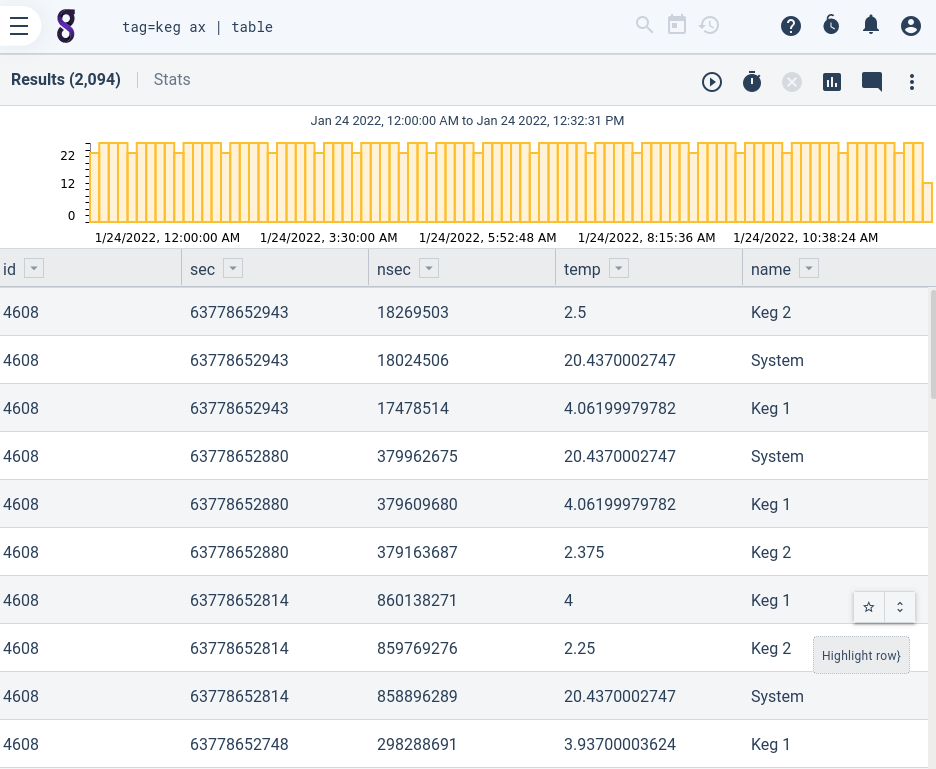
\includegraphics[width=0.65\linewidth]{images/sliced-keg.png}
	\caption{Sliced binary data}
	\label{fig:sliced-keg}
\end{figure}

From the manual query it is possible to derive the following
auto-extraction configuration:

\begin{Verbatim}[breaklines=true]
[[extraction]]
  tag="keg"
  name="kegdata"
  desc="binary temperature control extractions"
  module="slice"
  params="uint16be([0:2]) as id int64be([2:10]) as sec 
uint64be([10:18]) as nsec float32be([18:22]) as temp [22:] as name"
\end{Verbatim}

The complicated slice query now becomes:

\code{tag=keg ax \textbar{} table}

Using filtering in the ax module and some math modules it is now
possible to generate a graph showing the maximum temperature for each of
the probes, as shown in Figure \ref{fig:keg-temps}.

\begin{Verbatim}[breaklines=true]
tag=keg ax id==0x1200 temp name | max temp by name | chart max by name
\end{Verbatim}

\begin{figure}
	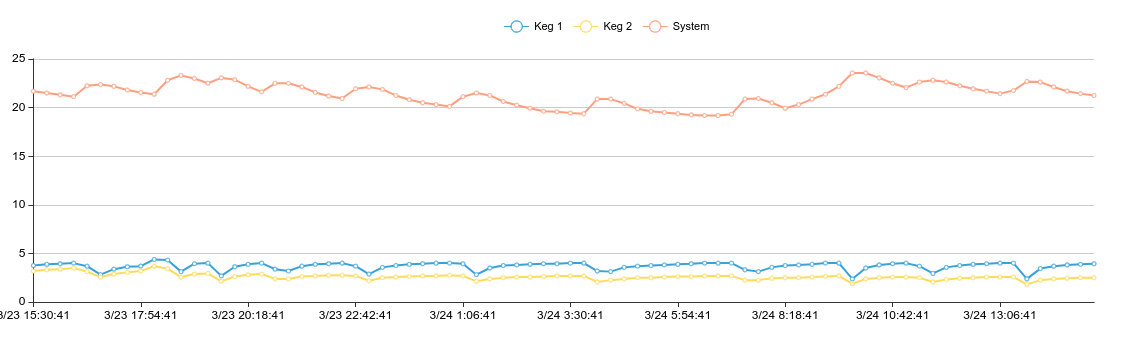
\includegraphics[width=0.65\linewidth]{images/keg-temps.png}
	\caption{Keg temperature graph}
	\label{fig:keg-temps}
\end{figure}

Additional filtering can be used to select only the keg temperatures
and examine the temperature variance to see how well the control system
is maintaining a constant temperature, as in Figure \ref{fig:keg-stddev}.

\begin{Verbatim}[breaklines=true]
tag=keg ax id==0x1200 temp name~Keg | stddev temp by name | chart stddev by name
\end{Verbatim}

\begin{figure}
	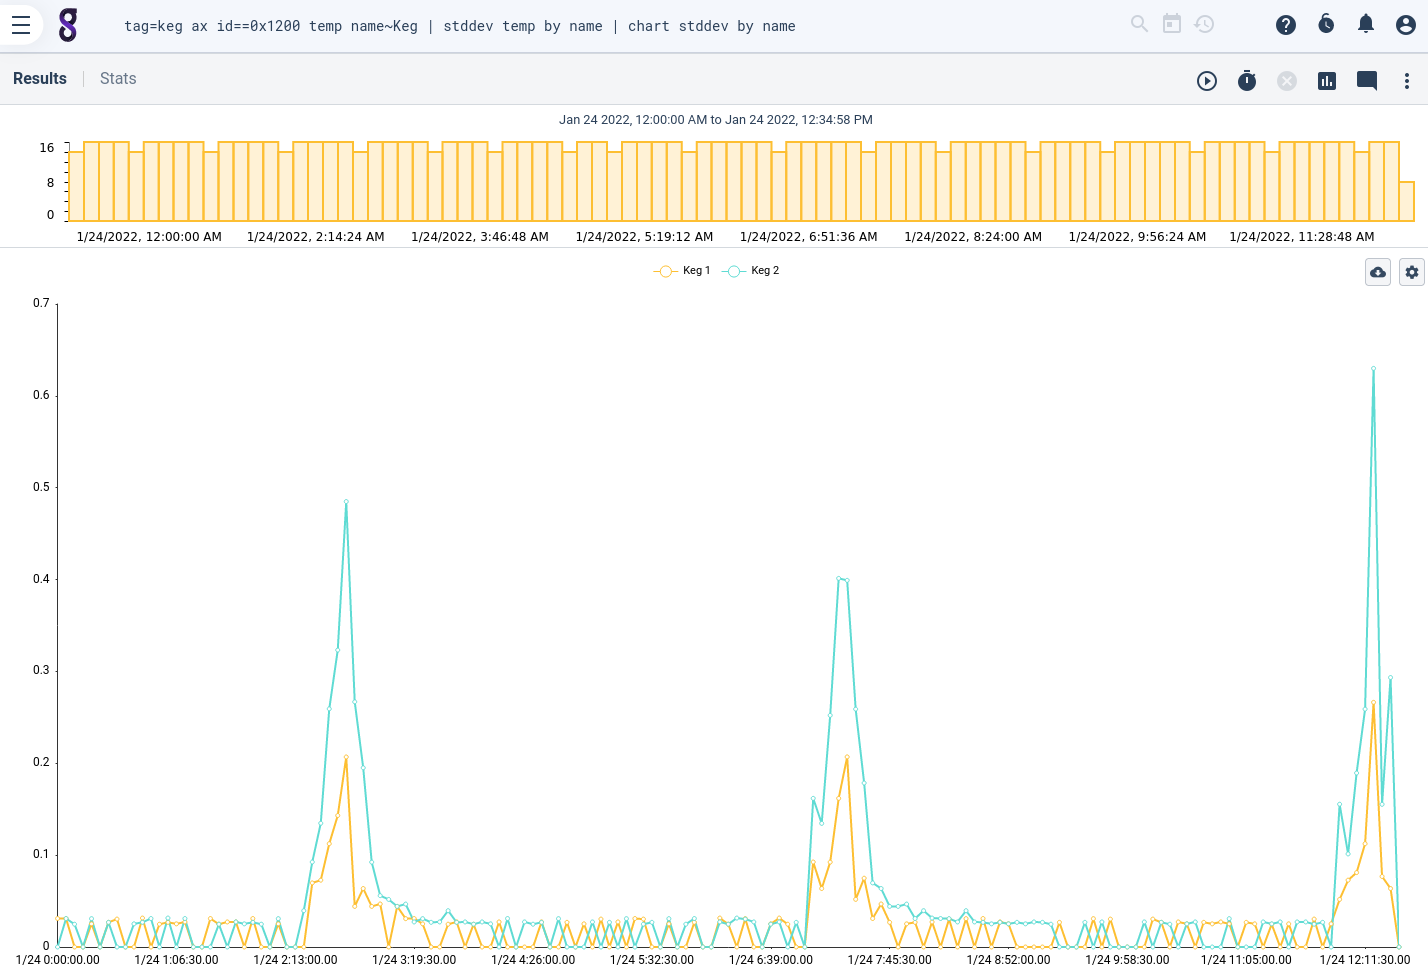
\includegraphics[width=0.65\linewidth]{images/keg-stddev.png}
	\caption{Keg standard deviation graph}
	\label{fig:keg-stddev}
\end{figure}

Using the auto-extractor and some basic math it is possible to dissect
the binary data and clearly see a periodic engagement of the compressor,
which causes an oscillation of temperature over time.

\clearpage
\subsection{Hands-On Lab: Extractors}

In this lab, we will show how to create an extractor to help work with
CSV data. First, launch a Gravwell webserver+indexer container:

\begin{Verbatim}[breaklines=true]
docker run --rm --net gravnet -p 8080:80 -d --name gravwell gravwell:base
\end{Verbatim}

Log into the web GUI (\href{http://localhost:8080}{http://localhost:8080}) and leave the page open.

Next, we'll use the ingester container image to run the CSV generator
tool. This will ingest 100 CSV-formatted entries under the tag ``csv'':

\begin{Verbatim}[breaklines=true]
docker run --rm --net gravnet --name ingesters -it -e \
GRAVWELL_CLEARTEXT_TARGETS=gravwell:4023 gravwell:ingesters \
/opt/gravwell/bin/csvGenerator -clear-conns gravwell:4023 -tag-name csv
\end{Verbatim}

A quick search on the csv tag should show the raw entries, as in Figure \ref{fig:lab-csv-raw}.

\code{tag=csv}

\begin{figure}
	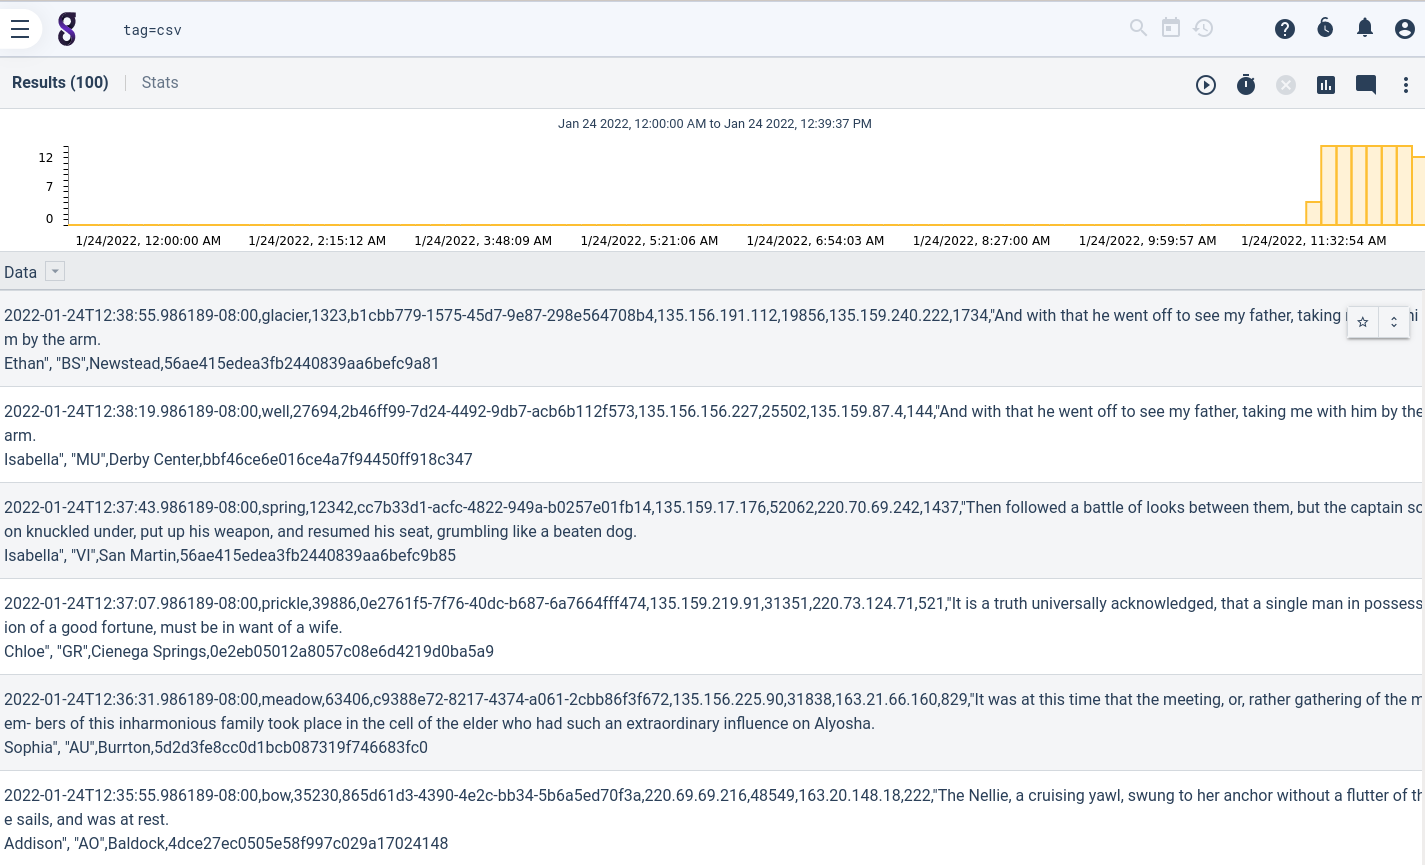
\includegraphics[width=0.7\linewidth]{images/lab-csv-raw.png}
	\caption{Raw CSV entries}
	\label{fig:lab-csv-raw}
\end{figure}

We could manually pull out fields from these entries by specifying
arguments to the csv search module, but a faster way is to create an
extractor. First, we must gather the necessary components to build an
extractor:

\begin{itemize}
\tightlist
\item
  tag: ``csv''
\item
  name: We will name this extractor ``csv\_extract''
\item
  description: ``CSV generator extraction''
\item
  module: ``csv''
\item
  params: Here we must decide what to call each column of CSV entries.
  Based on our knowledge of the CSV generator, we know the columns are:
  a timestamp, an ``application name'', a random integer ID, a UUID,
  an IP address, a number which could be a TCP port, another IP, another
  port, a quote from a piece of literature, a country code, a city name,
  and a hex-encoded IP address. From this we will decide to name the
  columns ``ts, app, id, uuid, ipA, portA, ipB, portB, msg, country,
  city, hexIP''
\item
  args: none needed.
\end{itemize}

Open the menu in the Gravwell UI, then select the ``Extractors'' page.
Click the ``Add'' button and populate it with the values above as shown in Figure \ref{fig:lab-new-extractor}

\begin{figure}
	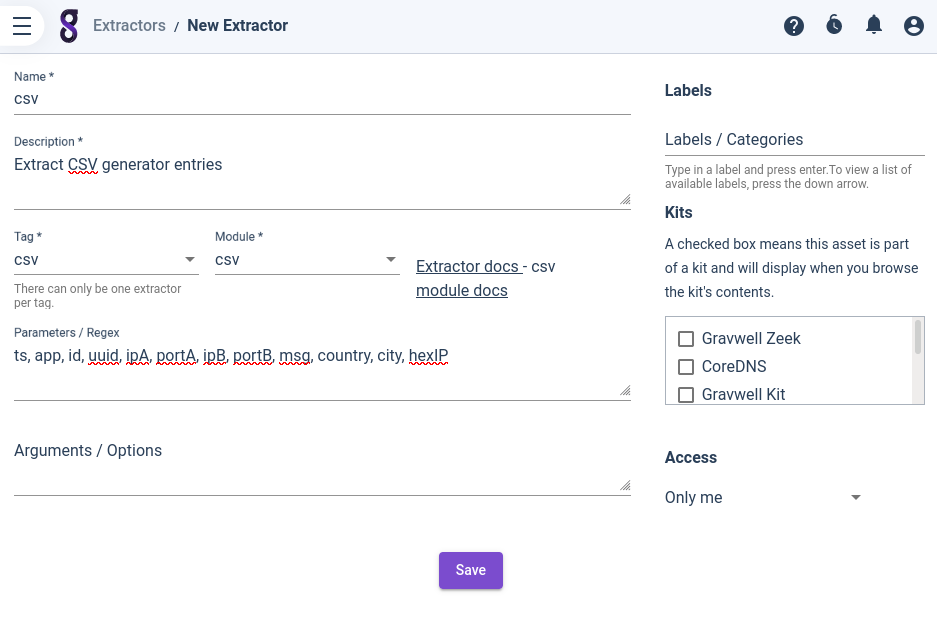
\includegraphics[width=0.8\linewidth]{images/new-extractor.png}
	\caption{Creating a new extractor}
	\label{fig:lab-new-extractor}
\end{figure}

We can test it by running the query \code{tag=csv ax \textbar{}
table}, which will extract and display all fields. The results should resemble Figure \ref{fig:lab-test-ax}.

\begin{figure}
	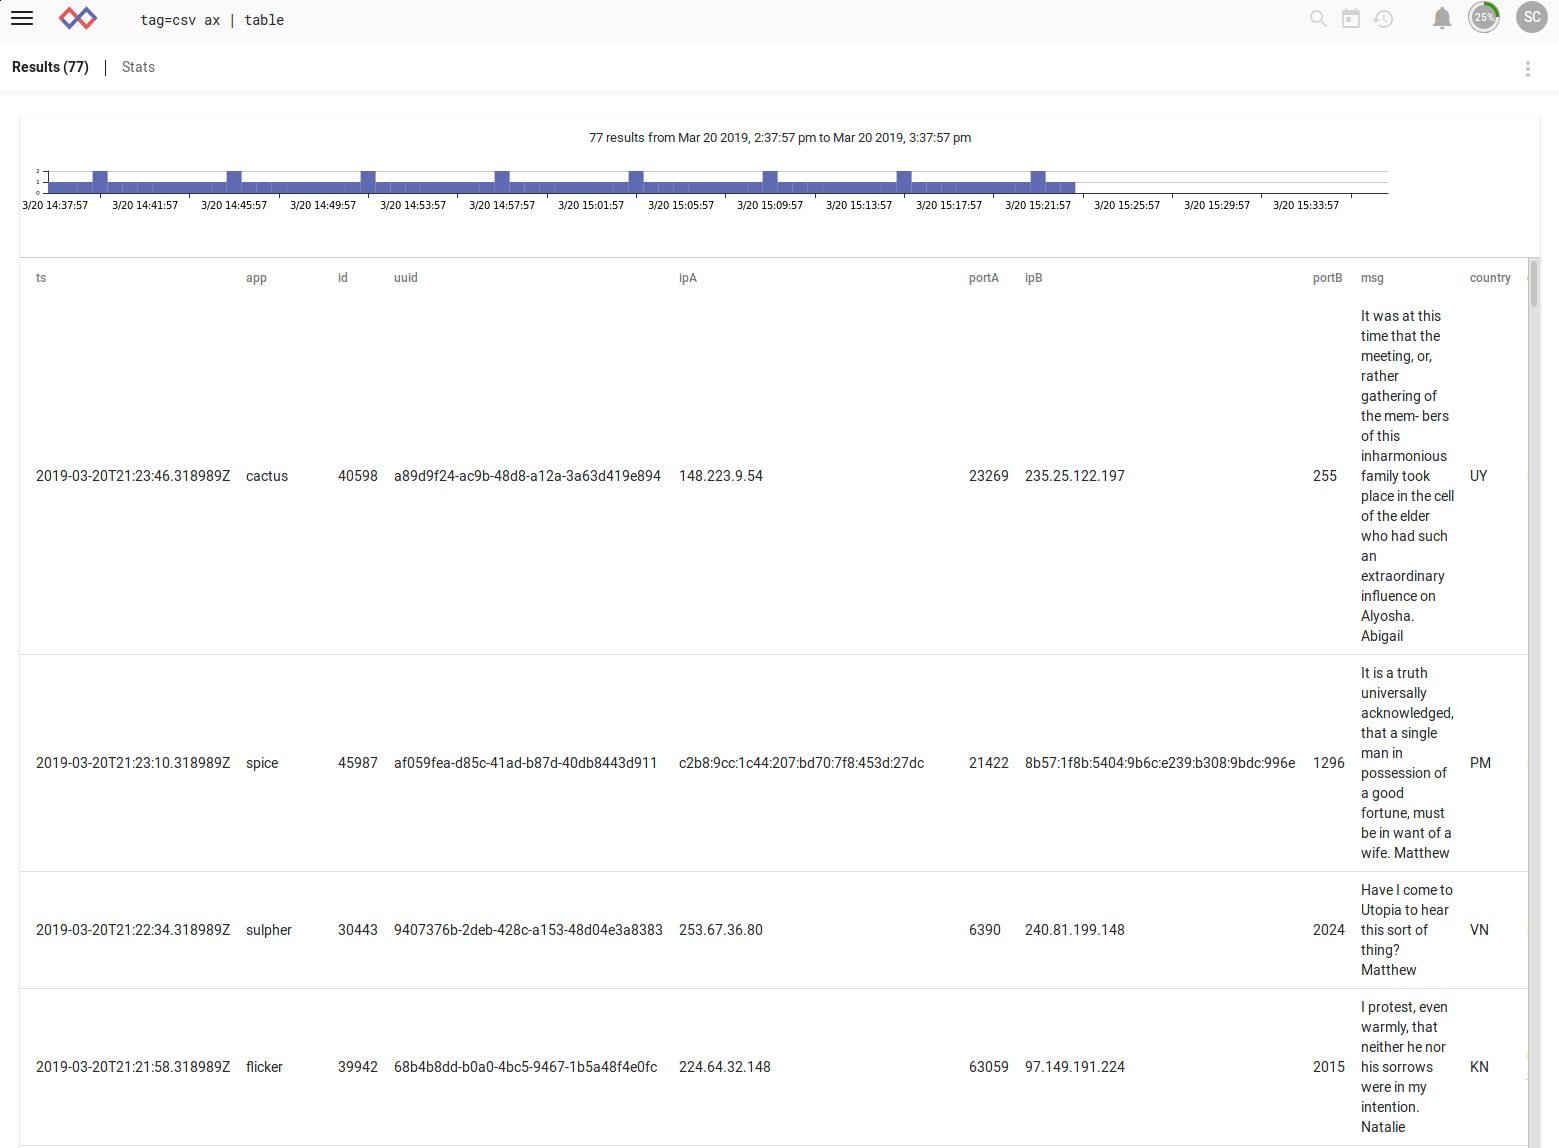
\includegraphics[width=0.8\linewidth]{images/lab-test-ax.png}
	\caption{Testing new extraction}
	\label{fig:lab-test-ax}
\end{figure}

To clean up after the experiment, run:

\begin{Verbatim}[breaklines=true]
docker kill $(docker ps -a -q)
\end{Verbatim}



\section{Backgrounded and Saved Searches}
\index{Search!background searches}\index{Search!saved searches}
Backgrounding a search allows a user to do other things while a search
completes--it is conceptually similar to running a Unix command with
an `\&' at the end of the command line. Searches can be launched in the
background by selecting the `Background Search' button on the New Search
page, as seen in Figure \ref{fig:bg-new-search}.


\begin{figure}
	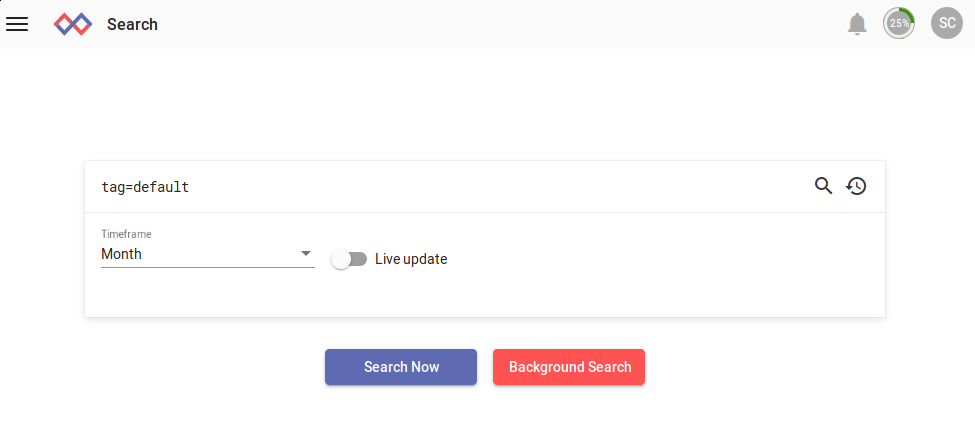
\includegraphics[width=0.8\linewidth]{images/bg-new-search.png}
	\caption{Starting a search in the background}
	\label{fig:bg-new-search}
\end{figure}

Or a running search can be sent to the background from the menu, as in Figure \ref{fig:bg-existing-search}.

\begin{figure}
	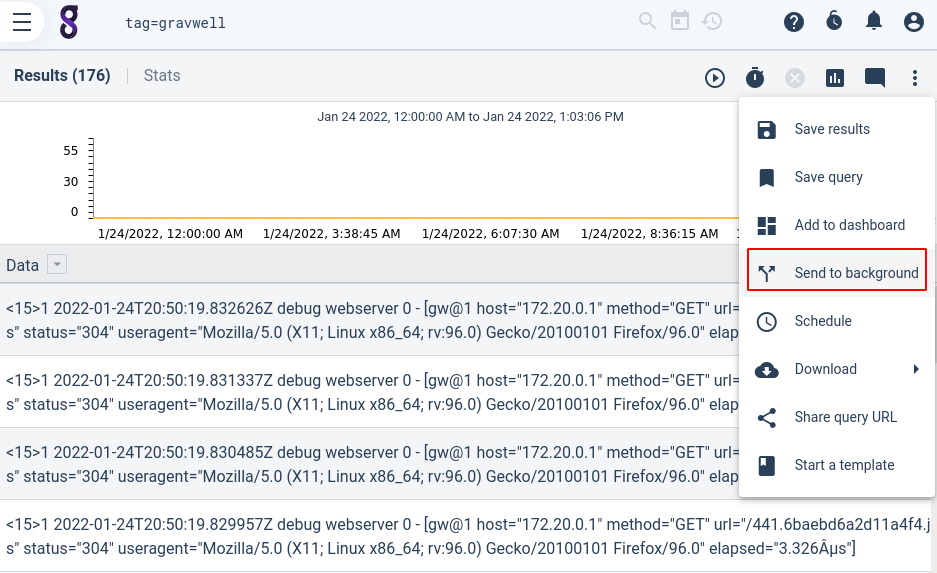
\includegraphics[width=0.8\linewidth]{images/bg-existing-search.png}
	\caption{Backgrounding a running search}
	\label{fig:bg-existing-search}
\end{figure}

In either case, backgrounding a search frees the user to do other
things while the search runs. The results of the search can later be
viewed in the Persistent Searches page (Figure \ref{fig:persistent-searches}).

\begin{figure}
	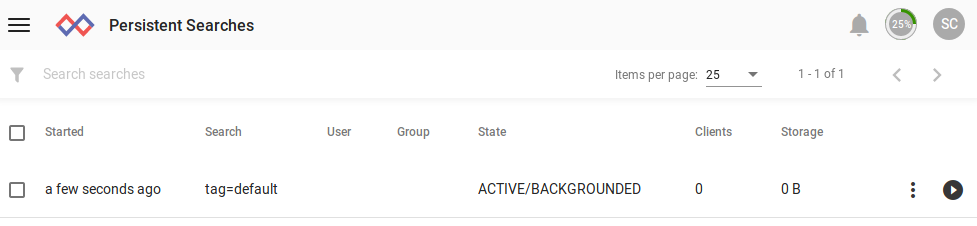
\includegraphics[width=0.8\linewidth]{images/persistent-searches.png}
	\caption{Persistent searches page}
	\label{fig:persistent-searches}
\end{figure}

Note that a backgrounded search is not guaranteed to persist across
server restarts. To keep the results of a search permanently, either
select `Save' in the search's menu on the Persistent Searches page (Figure \ref{fig:save-search}) or select `Save Results' from the menu on the search results page (Figure \ref{fig:save-search-menu}).

\begin{figure}
	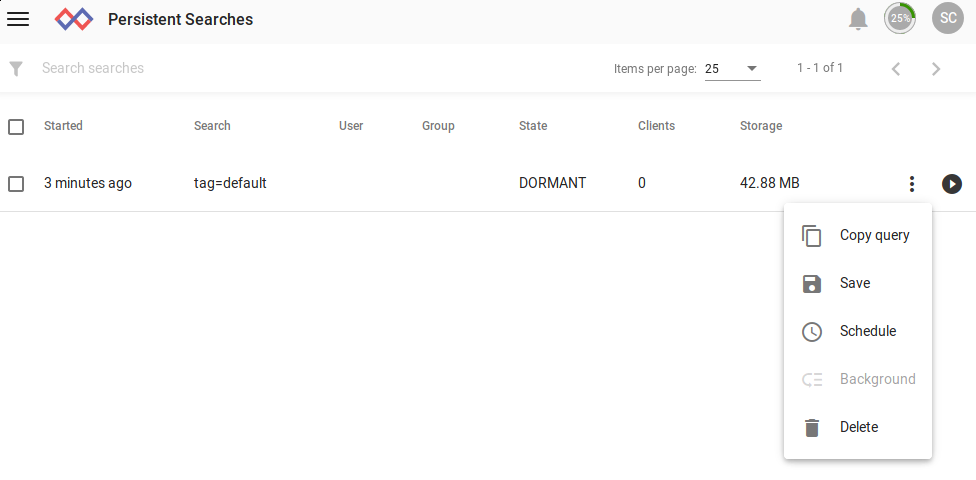
\includegraphics[width=0.8\linewidth]{images/save-search.png}
	\caption{Saving a search from the persistent searches page}
	\label{fig:save-search}
\end{figure}


\begin{figure}
	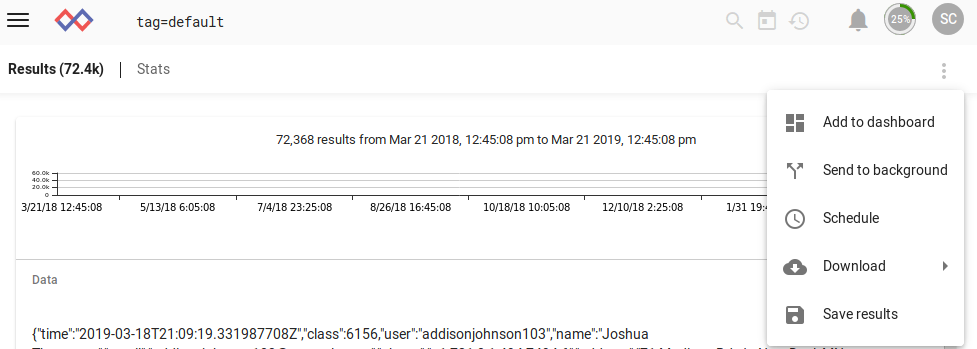
\includegraphics[width=0.8\linewidth]{images/save-search-menu.png}
	\caption{Saving a search from the search results page}
	\label{fig:save-search-menu}
\end{figure}

Be aware that saved searches take up space on the disk, and the
Gravwell administrator may choose to place restrictions on how much disk
space users are allowed to consume for search storage. It is good
practice to delete old saved searches when no longer needed!

\clearpage
\section{Permissions, Groups, and Sharing Results}

Any given user may belong to multiple groups, which are assigned by the
administrator. Users can then choose to share their search results,
dashboards, resources, and other things within the Gravwell system with
members of a particular group. In general, if something can be shared
with a group, the GUI will show a list of checkboxes, one per group.
Checking the box shares the item with that group.

The administrator creates groups on the admin-only Groups
administration page. In Figure \ref{fig:newgroup-foo}, the administrator is
creating a group named ``foo'' which contains the users John and Bob.

\begin{figure}
	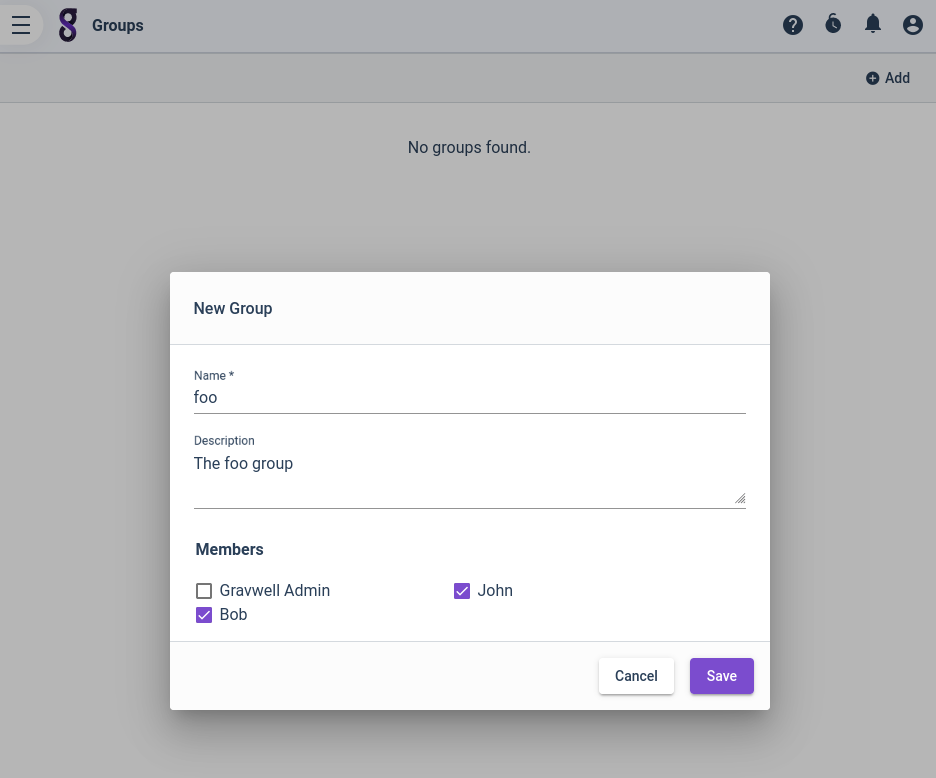
\includegraphics[width=0.8\linewidth]{images/newgroup-foo.png}
	\caption{Creating a new group}
	\label{fig:newgroup-foo}
\end{figure}

{}

Users can share the results of a search with a group from the
Persistent Searches page by selecting the `Edit group' button for that
search, as shown in Figure \ref{fig:share-search}.

\begin{figure}
	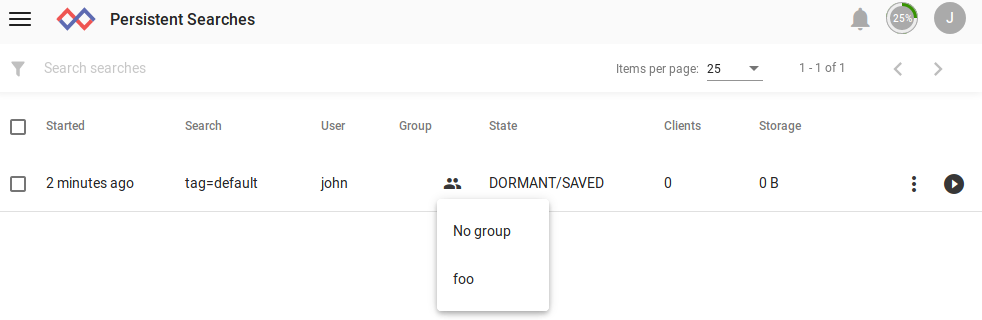
\includegraphics[width=0.7\linewidth]{images/share-search.png}
	\caption{Sharing search results}
	\label{fig:share-search}
\end{figure}

Once shared with a group, all members of that group will see the search
in their Persistent Searches listings. A user may optionally select a
default group for all their searches; this means every search the user
performs will by default be visible to members of that group. This can
be set from the Preferences tab of the Account page (Figure \ref{fig:default-group}).

\begin{figure}
	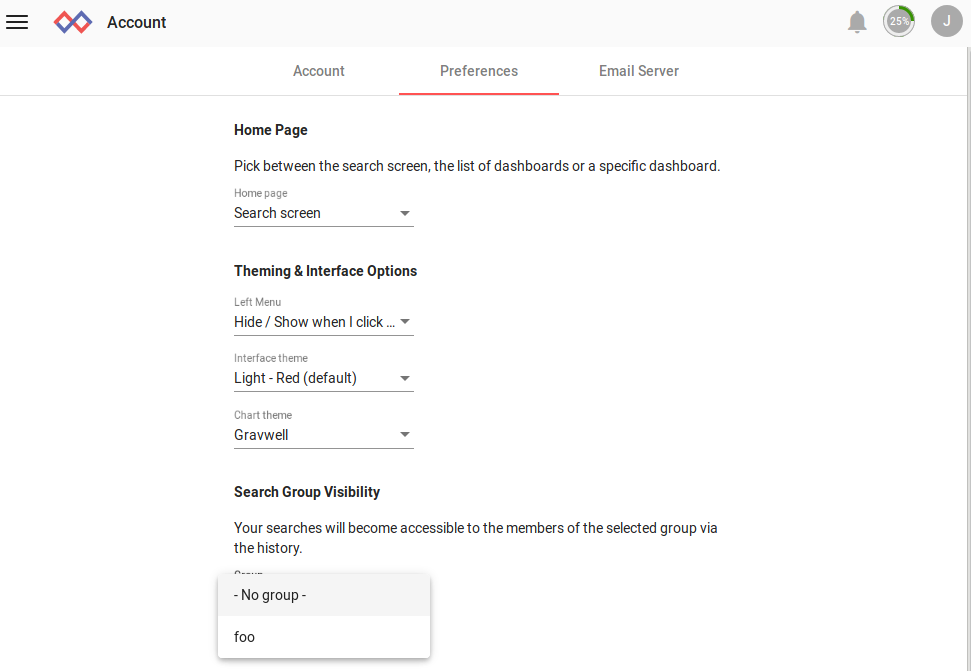
\includegraphics[width=0.7\linewidth]{images/default-group.png}
	\caption{Setting default group}
	\label{fig:default-group}
\end{figure}

\clearpage
\subsection{Hands-On Lab: Groups and Sharing}

This lab will demonstrate user groups and search result sharing. First,
launch a Gravwell webserver+indexer container:

\begin{Verbatim}[breaklines=true]
docker run --rm --net gravnet -p 8080:80 -d --name gravwell gravwell:base
\end{Verbatim}

Next, we'll use the ingesters container to feed some entries into the
indexer using the JSON generator:

\begin{Verbatim}[breaklines=true]
docker run --net gravnet --rm -i --name ingesters gravwell:ingesters \
/opt/gravwell/bin/jsonGenerator -clear-conns gravwell:4023
\end{Verbatim}

Now, log in as the administrator (\href{http://localhost:8080}{http://localhost:8080}), open the Users page, and add two new
users named `john' and `bob'. Use any passwords you like. Once you've
created the new users, you should see three users in the User page, as in Figure \ref{fig:lab-john-bob}.

\begin{figure}
	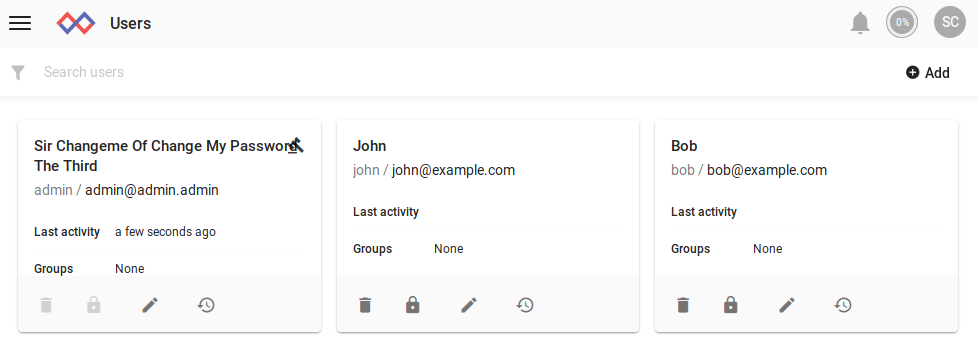
\includegraphics[width=0.7\linewidth]{images/lab-john-bob.png}
	\caption{Additional user accounts}
	\label{fig:lab-john-bob}
\end{figure}

Then open the Groups page and add a new group called `Test' containing
those users, as shown in Figure \ref{fig:lab-test-group}.

\begin{figure}
	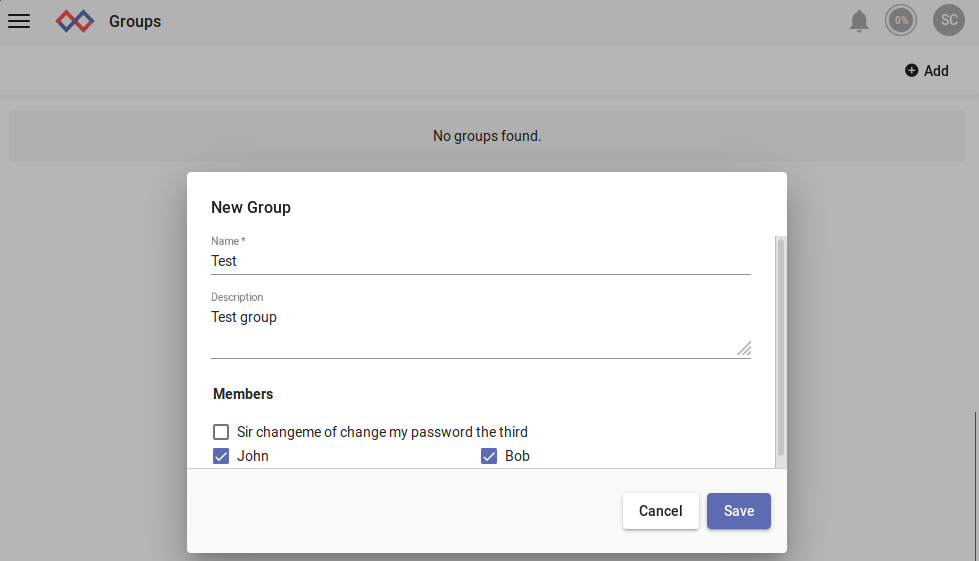
\includegraphics[width=0.7\linewidth]{images/lab-test-group.png}
	\caption{Creating a new test group}
	\label{fig:lab-test-group}
\end{figure}

With that complete, open a new Incognito/Private browser window and log
in as `john', then run the search \code{tag=json} over the last day. Save
the search, then go to the Persistent Searches page and make the search
accessible to the new Test group (Figure \ref{fig:lab-shared-search}).

\begin{figure}
	\includegraphics[width=0.7\linewidth]{images/lab-shared-search.png}
	\caption{Saved search shared with Test group}
	\label{fig:lab-shared-search}
\end{figure}

Close the Incognito window and open a new one, then log in as `bob'. Go
to the Persistent Searches page; you should see the saved search owned
by john. Open the saved search and verify that the contents are viewable by this
user.

To clean up after the experiment, run:

\begin{Verbatim}[breaklines=true]
docker kill $(docker ps -a -q)
\end{Verbatim}



\section{Dashboards}
\label{sec:dashboards}
\index{Dashboards}
Gravwell dashboards put relevant information in a
heads-up format suitable for continuous monitoring and situational
awareness. Dashboards are a collection of searches that are all executed in
parallel when the dashboard is loaded. The results are placed into tiles
which can be reordered or resized as desired.

Gravwell also supports ``live'' dashboards which automatically update
the search data. Under the hood, this is done by re-launching the
searches and swapping out the results when the new searches finish.

Dashboards are managed from the Dashboards page, as seen in Figure \ref{fig:dashboards}. 

\begin{figure}
	\includegraphics[width=0.8\linewidth]{images/dashboards.png}
	\caption{Dashboard management page.}
	\label{fig:dashboards}
\end{figure}

New dashboards can be created by clicking the ``Add'' button in the upper right; this brings up the dialog box in Figure \ref{fig:dashboard-add}. The dashboard needs a name, a description, and a default timeframe. By default, all queries run within a dashboard use the same timeframe.

\begin{figure}
	\includegraphics[width=0.6\linewidth]{images/dashboard-add.png}
	\caption{Creating a new dashboard.}
	\label{fig:dashboard-add}
\end{figure}

A newly-created dashboard is quite boring, as Figure \ref{fig:dashboard-blank} shows. There are two ways to add a new tile to a dashboard. Figure \ref{fig:add-to-dashboard} shows how to add a tile from the query results page: open the 3-dot menu, click ``Add to dashboard'', then find the desired dashboard in the list, select it, and optionally specify a new name for the tile.

\begin{figure}
	\includegraphics[width=0.8\linewidth]{images/dashboard-blank.png}
	\caption{An empty dashboard.}
	\label{fig:dashboard-blank}
\end{figure}

\begin{figure}
	\includegraphics[width=0.8\linewidth]{images/add-to-dashboard.png}
	\caption{Adding a search to a dashboard}
	\label{fig:add-to-dashboard}
\end{figure}

Figure \ref{fig:add-in-dashboard} shows how to add a tile from within the dashboard page: click the ``+'' icon on the page, then fill out the resulting dialog. The ``Query Settings'' portion is where the query will be selected; clicking the pencil icon will open a sub-dialog with many different query sources, as seen in Figure \ref{fig:query-settings}. Queries may be typed in directly, selected from the query library, and so on. In Figure \ref{fig:add-in-dashboard}, we have chosen to enter a query manually and selected the line chart renderer.


\begin{figure}
	\includegraphics[width=0.8\linewidth]{images/add-in-dashboard.png}
	\caption{Adding a tile to a dashboard}
	\label{fig:add-in-dashboard}
\end{figure}

\begin{figure}
	\includegraphics[width=0.6\linewidth]{images/query-settings.png}
	\caption{Query picker.}
	\label{fig:query-settings}
\end{figure}

Once a few tiles have been added to the dashboard, they can be rearranged and resized by clicking and dragging the tiles. Note that after making a change, you must click the ``Save changes'' popup which appears in the lower right corner.

\subsection{Live Update}
\index{Dashboards!live update}
Dashboards can be configured to \emph{live update}, meaning they will re-run queries and display new results after a set period of time. To enable this, click the 3-dot menu on the dashboard and select ``Settings''. Within the settings page, pick the ``Timeframe \& Live Update'' tab, then turn the ``Enable live update'' toggle on, as seen in Figure \ref{fig:live-update}. The update interval is configurable; if the queries in the dashboard cover a long timeframe or process a lot of data, consider setting the interval to a higher value so as to reduce the load on the system.

\begin{figure}
	\includegraphics[width=0.7\linewidth]{images/live-update.png}
	\caption{Live update settings.}
	\label{fig:live-update}
\end{figure}

\clearpage
\subsection{Hands-on Lab: Network Activity Dashboard}
\label{lab:dashboard}

For this exercise, we will be generating some Netflow data and creating
a dashboard to provide some awareness of network activity. Let's start
our docker containers for Gravwell, the netflow ingester, and a netflow
generator.

\begin{Verbatim}[breaklines=true]
docker run --rm --net gravnet -p 8080:80 -d --name gravwell gravwell:base

docker run --rm --net gravnet --name ingesters -it -e \
GRAVWELL_CLEARTEXT_TARGETS=gravwell:4023 gravwell:ingesters \
/opt/gravwell/bin/gravwell_netflow_capture

docker run -it --net gravnet --rm \
networkstatic/nflow-generator -t ingesters -p 2055
\end{Verbatim}

With Netflow data flowing in we can start to get our queries ready for
addition to a dashboard. The goal of this dashboard is to break down
network communications in some nice visuals that help us understand, at
a glance, what the most common hosts are, what traffic is being
utilized, where that traffic is going geographically, and potentially
other data.

Let's start by running a search to show a chart of traffic by port so we can
see which services are most used on our network:

\begin{Verbatim}[breaklines=true]
tag=netflow netflow Port Bytes | stats sum(Bytes) by Port | chart sum by Port
\end{Verbatim}

Now, use the menu button in the upper right of the search results page to select ``Add to
dashboard''. We have the option to create a fresh dashboard right from
here, so let's do so (Figure \ref{fig:new-dashboard}).

\begin{figure}
	\includegraphics[width=0.7\linewidth]{images/new-dashboard.png}
	\caption{Adding search to a new dashboard}
	\label{fig:new-dashboard}
\end{figure}

Click ``View Dashboard'' from the resulting popup message after you
save. You should see the newly-created dashboard with the chart sitting nicely in a
tile. Let's add one more search. Use the main menu to return to the new search page.
This time, let's get a table together of which hosts are communicating the most:

\begin{Verbatim}[breaklines=true]
tag=netflow netflow IP Bytes | stats sum(Bytes) by IP | table IP sum
\end{Verbatim}

Follow the same procedure to add this search to the dashboard but
instead of selecting ``New Dashboard'' you can choose the already
existing netflow dashboard. Give your tile a name like ``Top Talkers'',
click save, and then let's move back to the dashboard view.

It would be nice to let the user zoom in on a specific time area of
the dashboard results. This is accomplished by adding another tile as an
``Overview'' tile. The Overview renderer shows a chart of all log activity
and allows the user to click-drag and zoom in on specific regions for
more detail. To add an Overview tile, open the dashboard, then click
the new tile button in the upper right.  Give it a name (``Overview''
works well) and set the query to any one of the existing queries in the
dashboard. Then chose ``Overview'' from the renderer dropdown.

Dashboards can optionally sync up zooming of searches so that a zoom
on one Overview renderer will cause all other tiles to zoom to the same
range. This is controlled by the ``Update all tiles when zooming'' toggle
option under the Settings page for the dashboard, in the ``Timeframe \&
Live Update'' section (see Figure \ref{fig:dashboard-settings}). Open settings, enable that option, save, and
then return to the dashboard view. Now try zooming in on a small region
of the overview chart to see the other tiles respond.

\begin{figure}
	\includegraphics[width=0.7\linewidth]{images/dashboard-settings.png}
	\caption{Live update and zoom sync options.}
	\label{fig:dashboard-settings}
\end{figure}

We should now have two tiles present that are showing us some information
about our network communication, as well as an `overview' tile which we
can use for time exploration. As a final task, change the dashboard to use
live updates. This will periodically refresh the underlying search data
to keep the latest information available without having to refresh the
page or manually re-run searches. Navigate to the dashboard's Settings
page and turn on the ``Enable live update'' toggle in the ``Timeframe
\& Live Update'' section (see Figure \ref{fig:dashboard-settings}). The default update interval of 10s is fine.
Now, if you watch the dashboard, you should see it automatically refresh
every 10 seconds.

To clean up after the experiment, run:

\begin{Verbatim}[breaklines=true]
docker kill $(docker ps -a -q)
\end{Verbatim}

\section{Templates}
\index{Search!templates}\index{Dashboards!templates}
Templates are stored Gravwell queries which require one or more variables to run. This lets you build advanced queries which can investigate a particular IP address. They are particularly effective when inserted into a dashboard (section \ref{sec:dashboards}), or when coupled with an actionable (\ref{sec:actionables}).

Templates are managed via the templates page, accessed through the main menu under the `Tools and Resources' section. A template consists of a name, a description, and the query itself. Inside the query, use words wrapped inside doubled percent signs to denote variables, e.g. \code{\%\%IPADDR\%\%} as seen in Figure \ref{fig:template-editor}.

\begin{figure}
	\includegraphics[width=0.9\linewidth]{images/template-editor.png}
	\caption{Editing a template}
	\label{fig:template-editor}
\end{figure}

Once defined, a template can be run directly from the templates page by clicking the search button. A dialog (Figure \ref{fig:template-prompt}) will open prompting the user to fill in the variable before launching the search. More often, though, a template is executed either by launching an actionable from search results, or in a dashboard.

\begin{figure}
	\includegraphics[width=0.6\linewidth]{images/template-prompt.png}
	\caption{Launching a template}
	\label{fig:template-prompt}
\end{figure}

Templates can be included in dashboards by selecting ``Templates'' in the ``Add query via'' dropdown when creating a new tile, as seen in Figure \ref{fig:dashboard-template}. When the dashboard is opened, the user is prompted for the variable values. Dashboards containing templates may also be launched from actionables (section \ref{sec:actionables}).

\begin{figure}
	\includegraphics[width=0.8\linewidth]{images/dashboard-template.png}
	\caption{Adding a template to a dashboard tile}
	\label{fig:dashboard-template}
\end{figure}

\section{Actionables}
\label{sec:actionables}
\index{Actionables}\index{Dashboards!actionables}
Actionables provide a way to create custom triggers and menus that key on any text rendered in a query and take one or more actions when selected. Similar to an HTML hyperlink, actionables can be used to open external URLs that key on data, but actionables can also be leveraged to submit new Gravwell queries, launch dashboards, and execute templates.

Actionables are created by specifying one or more regular expressions, along with one or more actions. Gravwell automatically parses all text rendered with the table and chart renderers, bringing up appropriate actionable context menues when the text is clicked, as seen in Figure \ref{fig:actionables-overview}.

\begin{figure}
	\includegraphics[width=0.7\linewidth]{images/actionables-overview.png}
	\caption{Actionables context menu}
	\label{fig:actionables-overview}
\end{figure}

Actionables are made up of two components - triggers, which are simply regular expressions that Gravwell uses to match on text, and actions, which are the actions that can be taken on a matched trigger. An actionable can contain multiple triggers and/or multiple actions.

To get started with actionables, first open the Actionables menu, found in the main menu. Actionables are listed by name, and it's possible for two actionables to have the same name. By allowing actionables to have the same name, Gravwell can automatically group like actionables from different sources. For example, both the Netflow and CoreDNS kits provide actionables for IP addresses, and both are named "IP Address", as shown in Figure \ref{fig:actionables-menu}.

\begin{figure}
	\includegraphics[width=0.8\linewidth]{images/actionables-menu.png}
	\caption{Actionables duplicate names}
	\label{fig:actionables-menu}
\end{figure}

To create an actionable, you must define \emph{actions} and, optionally, one or more \emph{triggers}.

\subsection{Actions}

Actions provide operations that can be executed on text. An actionable can contain any number of actions. Actions include opening URLs, launching other searches, and more.

\subsubsection{The \_VALUE\_ Variable}

Some actions use the text of a capture group from the trigger to be used in the action itself. For example, we can use the trigger regex to extract a particular word in a string:

\begin{verbatim}
The color is (?<color>.*)
\end{verbatim}

The capture group contents can then be used in a URL, using \code{\_VALUE\_} for the matched text, e.g. \code{https://en.wikipedia.org/wiki/\_VALUE\_}

The keyword \code{\_VALUE\_} is the default placeholder for the matched text, and can be changed in some actions.

\subsubsection{Action Types}

Gravwell provides several actions, and an actionable can use any or all actions in a single actionable. 

\begin{itemize}
\item Run a Query: This action runs a new query, replacing the string \code{\_VALUE\_} with whatever text was matched by the actionable.
\item Execute a Template: The template action runs a pre-made template, using the matched text as the input variable to the template. 
\item Launch a Dashboard: The launch dashboard action opens a dashboard. If the dashboard has template variables, the user is prompted to select which variable to populate with the matched text.
\item Open a URL: The URL action supports opening a new window/tab with a given URL and matched text, and additionally provides a set of timestamp options for providing the time range arguments from the search that the actionable triggered on.  The "Open in a modal" option opens the URL in a window within the current Gravwell instance, similar to an HTML iframe.
\item Run a Saved Query: Run a query from the Query Library. 
\end{itemize}

%![](actionables-dashboard.png)

\subsubsection{Triggers}

A trigger is a JavaScript regular expression that determines if an actionable should be displayed for any given piece of text. For instance, one might use \code{(?:[0-9]\{1,3\}\.)\{3\}[0-9]\{1,3\}} as the trigger to match an IPv4 address. A trigger can be configured to highlight all matching text in query results with an underlined hyperlink which opens the actionables menu when clicked (``Click + text selection''), or it can be configured so that the actionable menu only pops up when the user explicitly selects text which matches the regular expression (``Text selection''). Figure \ref{fig:trigger} shows an example of a trigger on an actionable which will make any IPv4 addresses clickable.

\begin{figure}
	\includegraphics[width=0.9\linewidth]{images/trigger.png}
	\caption{Example actionable trigger.}
	\label{fig:trigger}
\end{figure}

\clearpage

\section{Compound Queries}
\label{sec:compoundqueries}
\index{Compound queries}\index{Search!compound queries}
Compound Queries is an extension to the query language that allows you to
perform multiple, in-order, queries, and use the output from a previous query
anywhere in the pipeline of the next, similar to an SQL JOIN. You can combine
multiple queries together as a single "compound" query in order to leverage
multiple data sources, fuse data into another query, and simplify complex
queries. Gravwell's compound query syntax is a simple sequence of in-order
queries, with additional notation to create temporary resources that can be
referenced in queries later in the sequence.

A compound query consists of a main query (the last query in a sequence), and
one or more inner queries. The main query is written just like a normal query,
while inner queries are always wrapped in the notation
\code{@<identifier>\{<query>\}}.  Queries are separated by a semicolon and
whitespace is ignored.

\begin{figure}
	\includegraphics[width=0.9\linewidth]{images/compound-breakdown.png}
	\caption{Parts of a compound query}
	\label{fig:compound-breakdown}
\end{figure}

For example, below is a compound query that has 2 inner queries and a main
query. 

\begin{verbatim}
@Q1{tag=default grep foo | json foo.bar foo.data};
@Q2{tag=syslog ax | table Event Payload};

tag=default ax 
| lookup -r @Q1 match bar bar data 
| lookup -r @Q2 Event Event Payload
\end{verbatim}

Inner queries generate named resources in the form of \code{@<identifier>}.
These can be used as regular resources with any module that supports
table-based resources. Supported modules are shown in table
\ref{table:supported-modules}. Unlike real resources however, named resources
in a compound query are ephemeral and scoped - they exist only while the query
is running and are visible only to compound query in which they were created.

\begin{table}[H]
\begin{tabular}{ | p{0.15\linewidth} | p{0.4\linewidth} | }
\hline
\textbf{Module} & \textbf{Notes}\\
dump & \\
\hline
enrich & \\
\hline
ipexist & Inner queries must use the table module with the -format ipexist flag \\
\hline
iplookup & Inner queries must use the table module with the -format csv flag \\
\hline
lookup & \\
\hline
anko & Anko scripts can read from named resources \\
\hline
\end{tabular}
	\caption{Supported modules that can use compound query resources}
\label{table:supported-modules}
\end{table}

Named resources are scoped to the compound query they exist in, and are
ephemeral - they are only accessible to other queries in the compound query,
and are deleted as soon as the query is completed.

For example, say we have both DNS query and IP-level connection data under the
tags "dns" and "conns", and we want to filter connection data down to only
connections that \emph{didn't} first have a corresponding DNS query; these are potentially suspicious IP addresses, since users typically access services via DNS names. We can use
compound queries to enrich our first query with DNS data and filter.

Let's start with the inner query:

\begin{verbatim}
tag=dns json query answers | table query answers
\end{verbatim}

This produces a table seen in Figure \ref{fig:compound-table1}

\begin{figure}
	\includegraphics[width=0.8\linewidth]{images/compound-table1.png}
	\caption{The beginning of an inner query}
	\label{fig:compound-table1}
\end{figure}

In the inner query, we simply create a table of all queries and answers in our
DNS data. Since this is an inner query, we need to give it a name so later
queries can reference its output, and wrap the query in braces. We'll call this
inner query "dns":

\begin{verbatim}
@dns{tag=dns json query answers | table query answers} 
\end{verbatim}

In the main query, we use our connection data, and use the lookup module to
read from our inner query "@dns":

\begin{verbatim}
tag=conns json SrcIP DstIP SrcIPBytes DstIPBytes 
| lookup -s -v -r @dns SrcIP answers query 
| table SrcIP DstIP SrcIPBytes DstIPBytes 
\end{verbatim}

This query uses the lookup module drop (via the -s and -v flags) any entry in
our conns data that has a SrcIP that matches a DNS answer. From there we simply
create a table of our data.

We wrap this into a compound query simply by joining the queries together and
separating them with a semicolon:

\begin{verbatim}
@dns{ tag=dns json query answers | table query answers };

tag=conns json SrcIP DstIP SrcIPBytes DstIPBytes 
| lookup -s -v -r @dns SrcIP answers query 
| table SrcIP DstIP SrcIPBytes DstIPBytes 
\end{verbatim}

This gives us a table (Figure \ref{fig:compound-table2} of just those connections that \emph{didn't} have a corresponding DNS
query.

\begin{figure}
	\includegraphics[width=0.8\linewidth]{images/compound-table2.png}
	\caption{Results from a complete compound query}
	\label{fig:compound-table2}
\end{figure}

